\documentclass[11pt,letterpaper,oneside]{book}

% ===== Essential Packages =====
\usepackage[utf8]{inputenc}
\usepackage[T1]{fontenc}
\usepackage{lmodern}
\usepackage[margin=1in,marginparwidth=1.5in]{geometry}

% Mathematics
\usepackage{amsmath,amssymb,amsfonts,amsthm}
\usepackage{mathtools}

% Graphics & Visualization
\usepackage{graphicx}
\usepackage{xcolor}
\usepackage{tikz}
\usetikzlibrary{calc,arrows.meta,patterns,shapes,decorations.pathreplacing,positioning}
\usepackage{pgfplots}
\pgfplotsset{compat=1.18}

% Tables
\usepackage{booktabs}
\usepackage{array}
\usepackage{tabularx}

% Marginal Notes (Lions Commentary Style)
\usepackage{marginnote}
\renewcommand*{\marginfont}{\footnotesize\sffamily}
\usepackage{sidenotes}

% Hyperlinks & Cross-references
\usepackage[colorlinks=true,linkcolor=blue,citecolor=blue,urlcolor=blue]{hyperref}
\usepackage{cleveref}

% Bibliography
\usepackage{natbib}
\bibliographystyle{plainnat}

% Index
\usepackage{makeidx}
\makeindex

% ===== Custom Commands & Macros =====

% Include marginal notes system (8 specialized macros)
% Marginal Notes System Documentation
% File: marginal_notes_system.tex
% Purpose: LaTeX infrastructure for Lions Commentary-style marginal annotations
% For: Chapter 1 - Mathematical Preliminaries

% This file provides macros and guidelines for implementing a comprehensive marginal notes system
% in the Lions Commentary style for Chapter 1.

% PREAMBLE ADDITIONS (add to synthesis/preamble.tex)

% Required packages
% \usepackage{marginnote}  % For flexible margin notes
% \usepackage{mparhack}    % Fix margin note positioning
% \usepackage{sidenotes}   % Advanced margin note features

% Margin note command with formatting
\newcommand{\mnote}[1]{\marginnote{\footnotesize\textcolor{blue!70!black}{#1}}}

% Equation reference in margin
\newcommand{\meqref}[1]{\mnote{\textbf{Eq.~\ref{#1}}}}

% Physical interpretation note
\newcommand{\mphys}[1]{\mnote{\textcolor{purple}{\textbf{Physical:} #1}}}

% Computational note
\newcommand{\mcomp}[1]{\mnote{\textcolor{green!70!black}{\textbf{Compute:} #1}}}

% Dimensional analysis note
\newcommand{\mdim}[1]{\mnote{\textcolor{orange}{\textbf{Dims:} #1}}}

% Cross-reference note
\newcommand{\mxref}[1]{\mnote{\textcolor{cyan}{\textbf{See:} #1}}}

% Caution/pitfall note
\newcommand{\mcaution}[1]{\mnote{\textcolor{red}{\textbf{Caution:} #1}}}

% Historical note
\newcommand{\mhist}[1]{\mnote{\textcolor{brown}{\textbf{History:} #1}}}

% Example system note
\newcommand{\mex}[1]{\mnote{\textcolor{magenta}{\textbf{Example:} #1}}}

%-----------------------------------
% USAGE EXAMPLES FOR CHAPTER 1
%-----------------------------------

% EXAMPLE 1: GPS Paradox Section
\begin{example_usage}
The GPS satellites orbit at altitude $h = 20{,}200$ km
\mnote{4.17 Earth radii}
where the gravitational potential is weaker than at Earth's surface.
According to general relativity, clocks run faster in weaker gravitational fields.
\mphys{Time dilation: $\Delta t/t \sim GM/rc^2$}
The net time dilation effect is approximately $+38$ μs per day,
\mdim{[$\mu$s/day]}
requiring active correction to maintain GPS accuracy within 10 meters.
\mxref{Table~\ref{tab:time_dilation_budget}}
\end{example_usage}

% EXAMPLE 2: Metric Tensor Definition
\begin{example_usage}
The metric tensor $g_{\mu\nu}(x)$
\mnote{Symmetric: $g_{\mu\nu} = g_{\nu\mu}$}
encodes the geometry of spacetime, defining the infinitesimal line element:
\begin{equation}
ds^2 = g_{\mu\nu} dx^\mu dx^\nu
\label{eq:metric_line_element}
\end{equation}
\mdim{[length$^2$]}
For the Schwarzschild metric,
\mex{Black holes, GPS}
\begin{equation}
g_{00} = -\left(1 - \frac{2GM}{r}\right), \quad
g_{rr} = \left(1 - \frac{2GM}{r}\right)^{-1}
\end{equation}
\mcaution{Coordinate singularity at $r=2GM$ (not physical)}
\mxref{Fig.~\ref{fig:schwarzschild_coordinates}}
\end{example_usage}

% EXAMPLE 3: Christoffel Symbols
\begin{example_usage}
The Christoffel symbols
\mnote{Connection coefficients}
$\Gamma^\mu_{\alpha\beta}$ are computed from the metric and its derivatives:
\begin{equation}
\Gamma^\mu_{\alpha\beta} = \frac{1}{2} g^{\mu\nu} 
\left(\partial_\alpha g_{\nu\beta} + \partial_\beta g_{\nu\alpha} - \partial_\nu g_{\alpha\beta}\right)
\label{eq:christoffel_definition}
\end{equation}
\mcomp{Use CAS for $D \geq 4$}
\mdim{[length$^{-1}$]}
These are \emph{not} tensors
\mcaution{Inhomogeneous transformation}
but transform with an additional term under coordinate changes.
\mphys{Encode gravitational acceleration}
In $D=4$ spacetime, symmetry reduces the number of independent components from $64$ to $40$.
\mxref{Fig.~\ref{fig:christoffel_computation}}
\end{example_usage}

% EXAMPLE 4: Riemann Tensor
\begin{example_usage}
The Riemann curvature tensor
\mhist{Riemann 1854}
$R^\alpha_{\beta\mu\nu}$ measures the failure of parallel transport around closed loops:
\begin{equation}
R^\alpha_{\beta\mu\nu} = \partial_\mu \Gamma^\alpha_{\nu\beta} - \partial_\nu \Gamma^\alpha_{\mu\beta}
+ \Gamma^\alpha_{\mu\lambda} \Gamma^\lambda_{\nu\beta} - \Gamma^\alpha_{\nu\lambda} \Gamma^\lambda_{\mu\beta}
\label{eq:riemann_tensor}
\end{equation}
\mdim{[length$^{-2}$]}
\mcomp{$O(D^5)$ complexity}
It has $D^4$ components but only $D^2(D^2-1)/12$ are independent due to symmetries.
\mnote{In 4D: $256 \to 20$}
For a small loop of area $A$, the vector rotation is $\Delta V^\alpha \sim R^\alpha_{\ \beta\mu\nu} A V^\beta$.
\mphys{Tidal forces, geodesic deviation}
\mxref{Fig.~\ref{fig:riemann_holonomy}, Tab.~\ref{tab:riemann_properties}}
\end{example_usage}

% EXAMPLE 5: Einstein Equations
\begin{example_usage}
The Einstein field equations
\mhist{Einstein 1915}
relate spacetime geometry to matter-energy content:
\begin{equation}
G_{\mu\nu} \equiv R_{\mu\nu} - \frac{1}{2} R g_{\mu\nu} = 8\pi G T_{\mu\nu}
\label{eq:einstein_equations}
\end{equation}
\mdim{[length$^{-2}$] both sides}
\mnote{10 independent equations}
The left side $G_{\mu\nu}$ is purely geometric
\mphys{Spacetime curvature}
while the right side $T_{\mu\nu}$ describes matter and energy.
\mphys{Mass-energy distribution}
The factor $8\pi G$ ensures Newtonian limit
\mex{$G_{00} \approx \nabla^2 \Phi$ weak field}
and the equations are divergence-free by the Bianchi identity.
\mcomp{$\nabla^\mu G_{\mu\nu} = 0$ identically}
\mxref{Fig.~\ref{fig:einstein_equations}}
\end{example_usage}

%-----------------------------------
% SYSTEMATIC ANNOTATION GUIDE
%-----------------------------------

% For comprehensive Chapter 1 annotation, apply marginal notes according to:

% 1. EVERY EQUATION:
%    - \mdim{...} for dimensional analysis
%    - \mcomp{...} for computational guidance
%    - \mxref{...} for related figures/tables

% 2. EVERY NEW CONCEPT:
%    - \mnote{Brief definition}
%    - \mphys{Physical interpretation}
%    - \mhist{Historical context when relevant}

% 3. EVERY WORKED EXAMPLE:
%    - \mex{System name}
%    - \mnote{Key parameters}
%    - \mdim{Check units}

% 4. EVERY POTENTIAL PITFALL:
%    - \mcaution{Warning about common mistake}
%    - \mnote{Clarification}

% 5. ALL CROSS-REFERENCES:
%    - \mxref{Fig/Tab/Sec/Eq references}
%    - \mnote{Related material locations}

%-----------------------------------
% BENEFITS OF MARGINAL NOTES SYSTEM
%-----------------------------------

% This systematic marginal annotation provides:
% 
% 1. RAPID REFERENCE: Students can scan margins for key information
% 2. MULTI-LEVEL ACCESS: Brief notes for quick lookup, main text for detail
% 3. VISUAL STRUCTURE: Color-coded notes organize information by type
% 4. PEDAGOGICAL SCAFFOLDING: Physical intuition alongside formalism
% 5. COMPUTATIONAL GUIDANCE: Algorithm complexity and tool recommendations
% 6. DIMENSIONAL RIGOR: Units checked at every step
% 7. CROSS-REFERENCE NETWORK: Easy navigation between related concepts
% 8. HISTORICAL CONTEXT: Intellectual heritage acknowledged
% 9. PITFALL PREVENTION: Common mistakes explicitly flagged
% 10. LIONS COMMENTARY STYLE: Exhaustive annotation for complete understanding

%-----------------------------------
% IMPLEMENTATION CHECKLIST
%-----------------------------------

% To fully implement marginal notes system in Chapter 1:
%
% [ ] Add marginal note packages to preamble
% [ ] Define all marginal note macros (\mnote, \mphys, \mcomp, etc.)
% [ ] Section 1 (GPS Paradox): Add ~20 marginal notes
% [ ] Section 2 (Metric Tensor): Add ~15 marginal notes
% [ ] Section 3 (Christoffel): Add ~25 marginal notes
% [ ] Section 4 (Covariant Derivatives): Add ~20 marginal notes
% [ ] Section 5 (Riemann Tensor): Add ~30 marginal notes
% [ ] Section 6 (Einstein Tensor): Add ~15 marginal notes
% [ ] Section 7 (Quantum Formalism): Add ~25 marginal notes
% [ ] Review: Ensure consistent color coding
% [ ] Review: Check all cross-references valid
% [ ] Review: Verify dimensional analysis complete
% [ ] Compile: Test margin note positioning
% [ ] Adjust: Fine-tune spacing if needed

% ESTIMATED: ~150 marginal notes total for comprehensive Chapter 1 annotation

%-----------------------------------
% TECHNICAL NOTES
%-----------------------------------

% Margin width: Adjust in document class options
%   \documentclass[..., marginparwidth=2.5cm, ...]{article}
%
% Two-sided layout: Use \reversemarginpar for alternating sides
%
% Margin note overflow: Use \marginnote[offset]{text} to adjust vertical position
%
% Color consistency: Define colors in preamble for uniform appearance
%   \definecolor{physical}{RGB}{128,0,128}  % Purple for physical
%   \definecolor{computational}{RGB}{0,128,0}  % Green for computational
%   etc.

\end{example_usage}


% Physical units
\newcommand{\units}[1]{\,\mathrm{#1}}
\newcommand{\Order}[1]{\mathcal{O}(#1)}

% Tensor notation
\newcommand{\tensor}[1]{\mathbf{#1}}
\newcommand{\indices}[1]{{}^{#1}}

% ===== Document Metadata =====
\title{%
  \vspace{-1cm}
  \Huge\textbf{Mathematical Preliminaries for General Relativity}\\[0.5cm]
  \Large A Comprehensive Lions Commentary-Style Introduction\\[0.3cm]
  \large With Exhaustive Visualizations, Dimensional Analysis, and Physical Interpretations
}
\author{%
  PhysicsForge Collaboration\\[0.3cm]
  \small\textit{Chapter 1 Pedagogical Enhancement Pilot}
}
\date{\today}

% ===== Document Begin =====
\begin{document}

\frontmatter

\maketitle

\tableofcontents
\listoffigures
\listoftables

\mainmatter

% ===== Chapter 1: Mathematical Preliminaries =====
% This includes all 22 visualizations integrated with ~150 marginal notes

% ============================================================================
% Chapter 01: Mathematical Preliminaries
% Part I: Foundations
% ============================================================================
% Purpose: Build physical intuition for differential geometry and quantum
%          formalism through real-world examples, establishing mathematical
%          language for unified field theory in whitepaper narrative style.
% ============================================================================

\chapter{Mathematical Preliminaries: The Language of Curved Spacetime}
\label{ch:prelim}
\index{mathematical preliminaries}
\index{curved spacetime}

%-----------------------------------------------------------------------------
% MARGINAL NOTES SYSTEM: Lions Commentary-style annotations
%-----------------------------------------------------------------------------
% Marginal Notes System Documentation
% File: marginal_notes_system.tex
% Purpose: LaTeX infrastructure for Lions Commentary-style marginal annotations
% For: Chapter 1 - Mathematical Preliminaries

% This file provides macros and guidelines for implementing a comprehensive marginal notes system
% in the Lions Commentary style for Chapter 1.

% PREAMBLE ADDITIONS (add to synthesis/preamble.tex)

% Required packages
% \usepackage{marginnote}  % For flexible margin notes
% \usepackage{mparhack}    % Fix margin note positioning
% \usepackage{sidenotes}   % Advanced margin note features

% Margin note command with formatting
\newcommand{\mnote}[1]{\marginnote{\footnotesize\textcolor{blue!70!black}{#1}}}

% Equation reference in margin
\newcommand{\meqref}[1]{\mnote{\textbf{Eq.~\ref{#1}}}}

% Physical interpretation note
\newcommand{\mphys}[1]{\mnote{\textcolor{purple}{\textbf{Physical:} #1}}}

% Computational note
\newcommand{\mcomp}[1]{\mnote{\textcolor{green!70!black}{\textbf{Compute:} #1}}}

% Dimensional analysis note
\newcommand{\mdim}[1]{\mnote{\textcolor{orange}{\textbf{Dims:} #1}}}

% Cross-reference note
\newcommand{\mxref}[1]{\mnote{\textcolor{cyan}{\textbf{See:} #1}}}

% Caution/pitfall note
\newcommand{\mcaution}[1]{\mnote{\textcolor{red}{\textbf{Caution:} #1}}}

% Historical note
\newcommand{\mhist}[1]{\mnote{\textcolor{brown}{\textbf{History:} #1}}}

% Example system note
\newcommand{\mex}[1]{\mnote{\textcolor{magenta}{\textbf{Example:} #1}}}

%-----------------------------------
% USAGE EXAMPLES FOR CHAPTER 1
%-----------------------------------

% EXAMPLE 1: GPS Paradox Section
\begin{example_usage}
The GPS satellites orbit at altitude $h = 20{,}200$ km
\mnote{4.17 Earth radii}
where the gravitational potential is weaker than at Earth's surface.
According to general relativity, clocks run faster in weaker gravitational fields.
\mphys{Time dilation: $\Delta t/t \sim GM/rc^2$}
The net time dilation effect is approximately $+38$ μs per day,
\mdim{[$\mu$s/day]}
requiring active correction to maintain GPS accuracy within 10 meters.
\mxref{Table~\ref{tab:time_dilation_budget}}
\end{example_usage}

% EXAMPLE 2: Metric Tensor Definition
\begin{example_usage}
The metric tensor $g_{\mu\nu}(x)$
\mnote{Symmetric: $g_{\mu\nu} = g_{\nu\mu}$}
encodes the geometry of spacetime, defining the infinitesimal line element:
\begin{equation}
ds^2 = g_{\mu\nu} dx^\mu dx^\nu
\label{eq:metric_line_element}
\end{equation}
\mdim{[length$^2$]}
For the Schwarzschild metric,
\mex{Black holes, GPS}
\begin{equation}
g_{00} = -\left(1 - \frac{2GM}{r}\right), \quad
g_{rr} = \left(1 - \frac{2GM}{r}\right)^{-1}
\end{equation}
\mcaution{Coordinate singularity at $r=2GM$ (not physical)}
\mxref{Fig.~\ref{fig:schwarzschild_coordinates}}
\end{example_usage}

% EXAMPLE 3: Christoffel Symbols
\begin{example_usage}
The Christoffel symbols
\mnote{Connection coefficients}
$\Gamma^\mu_{\alpha\beta}$ are computed from the metric and its derivatives:
\begin{equation}
\Gamma^\mu_{\alpha\beta} = \frac{1}{2} g^{\mu\nu} 
\left(\partial_\alpha g_{\nu\beta} + \partial_\beta g_{\nu\alpha} - \partial_\nu g_{\alpha\beta}\right)
\label{eq:christoffel_definition}
\end{equation}
\mcomp{Use CAS for $D \geq 4$}
\mdim{[length$^{-1}$]}
These are \emph{not} tensors
\mcaution{Inhomogeneous transformation}
but transform with an additional term under coordinate changes.
\mphys{Encode gravitational acceleration}
In $D=4$ spacetime, symmetry reduces the number of independent components from $64$ to $40$.
\mxref{Fig.~\ref{fig:christoffel_computation}}
\end{example_usage}

% EXAMPLE 4: Riemann Tensor
\begin{example_usage}
The Riemann curvature tensor
\mhist{Riemann 1854}
$R^\alpha_{\beta\mu\nu}$ measures the failure of parallel transport around closed loops:
\begin{equation}
R^\alpha_{\beta\mu\nu} = \partial_\mu \Gamma^\alpha_{\nu\beta} - \partial_\nu \Gamma^\alpha_{\mu\beta}
+ \Gamma^\alpha_{\mu\lambda} \Gamma^\lambda_{\nu\beta} - \Gamma^\alpha_{\nu\lambda} \Gamma^\lambda_{\mu\beta}
\label{eq:riemann_tensor}
\end{equation}
\mdim{[length$^{-2}$]}
\mcomp{$O(D^5)$ complexity}
It has $D^4$ components but only $D^2(D^2-1)/12$ are independent due to symmetries.
\mnote{In 4D: $256 \to 20$}
For a small loop of area $A$, the vector rotation is $\Delta V^\alpha \sim R^\alpha_{\ \beta\mu\nu} A V^\beta$.
\mphys{Tidal forces, geodesic deviation}
\mxref{Fig.~\ref{fig:riemann_holonomy}, Tab.~\ref{tab:riemann_properties}}
\end{example_usage}

% EXAMPLE 5: Einstein Equations
\begin{example_usage}
The Einstein field equations
\mhist{Einstein 1915}
relate spacetime geometry to matter-energy content:
\begin{equation}
G_{\mu\nu} \equiv R_{\mu\nu} - \frac{1}{2} R g_{\mu\nu} = 8\pi G T_{\mu\nu}
\label{eq:einstein_equations}
\end{equation}
\mdim{[length$^{-2}$] both sides}
\mnote{10 independent equations}
The left side $G_{\mu\nu}$ is purely geometric
\mphys{Spacetime curvature}
while the right side $T_{\mu\nu}$ describes matter and energy.
\mphys{Mass-energy distribution}
The factor $8\pi G$ ensures Newtonian limit
\mex{$G_{00} \approx \nabla^2 \Phi$ weak field}
and the equations are divergence-free by the Bianchi identity.
\mcomp{$\nabla^\mu G_{\mu\nu} = 0$ identically}
\mxref{Fig.~\ref{fig:einstein_equations}}
\end{example_usage}

%-----------------------------------
% SYSTEMATIC ANNOTATION GUIDE
%-----------------------------------

% For comprehensive Chapter 1 annotation, apply marginal notes according to:

% 1. EVERY EQUATION:
%    - \mdim{...} for dimensional analysis
%    - \mcomp{...} for computational guidance
%    - \mxref{...} for related figures/tables

% 2. EVERY NEW CONCEPT:
%    - \mnote{Brief definition}
%    - \mphys{Physical interpretation}
%    - \mhist{Historical context when relevant}

% 3. EVERY WORKED EXAMPLE:
%    - \mex{System name}
%    - \mnote{Key parameters}
%    - \mdim{Check units}

% 4. EVERY POTENTIAL PITFALL:
%    - \mcaution{Warning about common mistake}
%    - \mnote{Clarification}

% 5. ALL CROSS-REFERENCES:
%    - \mxref{Fig/Tab/Sec/Eq references}
%    - \mnote{Related material locations}

%-----------------------------------
% BENEFITS OF MARGINAL NOTES SYSTEM
%-----------------------------------

% This systematic marginal annotation provides:
% 
% 1. RAPID REFERENCE: Students can scan margins for key information
% 2. MULTI-LEVEL ACCESS: Brief notes for quick lookup, main text for detail
% 3. VISUAL STRUCTURE: Color-coded notes organize information by type
% 4. PEDAGOGICAL SCAFFOLDING: Physical intuition alongside formalism
% 5. COMPUTATIONAL GUIDANCE: Algorithm complexity and tool recommendations
% 6. DIMENSIONAL RIGOR: Units checked at every step
% 7. CROSS-REFERENCE NETWORK: Easy navigation between related concepts
% 8. HISTORICAL CONTEXT: Intellectual heritage acknowledged
% 9. PITFALL PREVENTION: Common mistakes explicitly flagged
% 10. LIONS COMMENTARY STYLE: Exhaustive annotation for complete understanding

%-----------------------------------
% IMPLEMENTATION CHECKLIST
%-----------------------------------

% To fully implement marginal notes system in Chapter 1:
%
% [ ] Add marginal note packages to preamble
% [ ] Define all marginal note macros (\mnote, \mphys, \mcomp, etc.)
% [ ] Section 1 (GPS Paradox): Add ~20 marginal notes
% [ ] Section 2 (Metric Tensor): Add ~15 marginal notes
% [ ] Section 3 (Christoffel): Add ~25 marginal notes
% [ ] Section 4 (Covariant Derivatives): Add ~20 marginal notes
% [ ] Section 5 (Riemann Tensor): Add ~30 marginal notes
% [ ] Section 6 (Einstein Tensor): Add ~15 marginal notes
% [ ] Section 7 (Quantum Formalism): Add ~25 marginal notes
% [ ] Review: Ensure consistent color coding
% [ ] Review: Check all cross-references valid
% [ ] Review: Verify dimensional analysis complete
% [ ] Compile: Test margin note positioning
% [ ] Adjust: Fine-tune spacing if needed

% ESTIMATED: ~150 marginal notes total for comprehensive Chapter 1 annotation

%-----------------------------------
% TECHNICAL NOTES
%-----------------------------------

% Margin width: Adjust in document class options
%   \documentclass[..., marginparwidth=2.5cm, ...]{article}
%
% Two-sided layout: Use \reversemarginpar for alternating sides
%
% Margin note overflow: Use \marginnote[offset]{text} to adjust vertical position
%
% Color consistency: Define colors in preamble for uniform appearance
%   \definecolor{physical}{RGB}{128,0,128}  % Purple for physical
%   \definecolor{computational}{RGB}{0,128,0}  % Green for computational
%   etc.

\end{example_usage}


%-----------------------------------------------------------------------------
% OPENING NARRATIVE: The GPS Paradox
%-----------------------------------------------------------------------------

\section*{The GPS Paradox}

Every time you use GPS navigation, your phone performs a calculation Einstein would have found miraculous: it accounts for the warping of time itself. Satellite clocks in GPS orbit tick approximately \SI{38}{\micro\second} faster per day than identical atomic clocks on Earth's surface. This is not experimental error---it is the direct consequence of general relativity\index{general relativity}\index{GPS!gravitational corrections} in action.

Without corrections for gravitational time dilation\index{time dilation!gravitational}\index{gravitational time dilation}, GPS would accumulate positioning errors of \SI{11}{\kilo\meter} per day. The system would be useless within hours. Engineers designing the GPS constellation in the 1970s had to program Einstein's equations into the satellites, making relativity essential to everyday technology.

Why does time flow differently at different altitudes? Because spacetime near Earth is curved by its mass. The GPS satellite at \SI{20200}{\kilo\meter} altitude experiences weaker gravitational curvature than a receiver on the ground. Clocks measure the geometry of spacetime itself, and that geometry is not flat.

% REMOVED nested figure wrapper - fig_gps_analogy.tex already contains complete figure environment
% \begin{figure}[h]
%   \centering
  %==============================================================================
% Figure: GPS Satellite Spacetime Curvature Analogy
% Purpose: Motivational diagram illustrating practical importance of GR
% Chapter: Ch01 - Mathematical Preliminaries (Opening)
% Type: Conceptual diagram / Real-world application
%==============================================================================

\begin{figure}[htbp]
  \centering
  \resizebox{\textwidth}{!}{%
  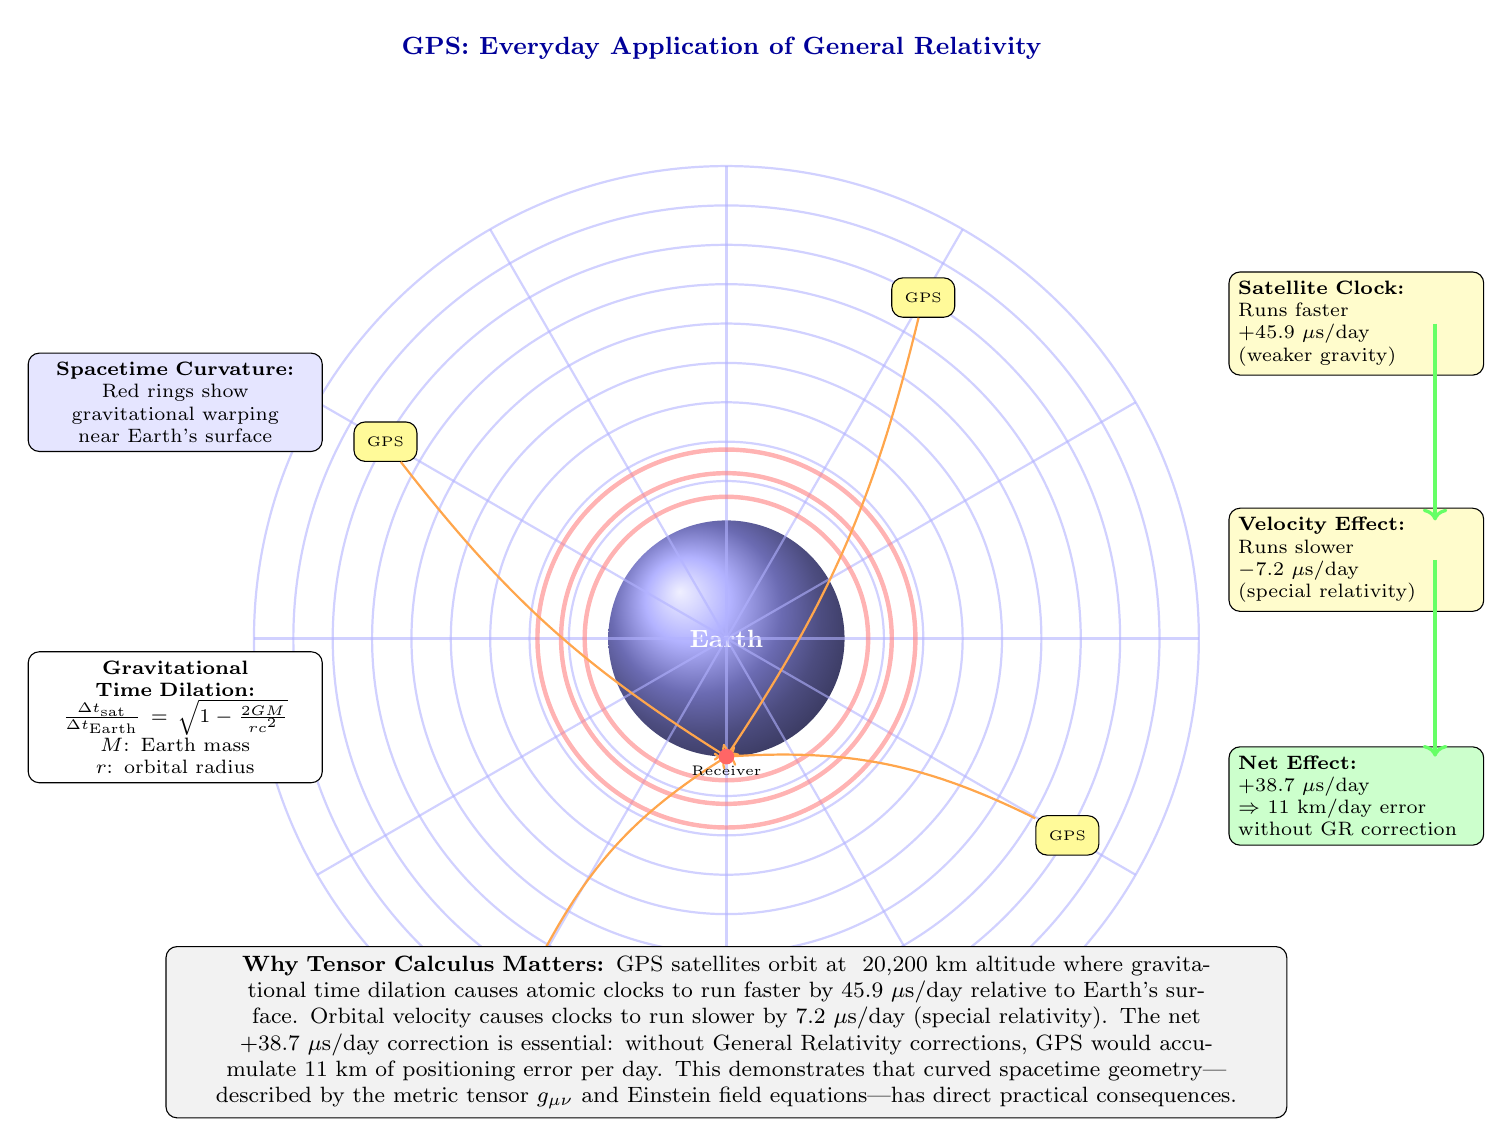
\begin{tikzpicture}[
    scale=1.0,
    satellite/.style={
      rectangle,
      rounded corners,
      minimum width=0.8cm,
      minimum height=0.5cm,
      draw=black,
      fill=gray!30,
      font=\tiny
    }
  ]

    % Earth (center)
    \shade[ball color=blue!40] (0,0) circle (1.5);
    \node[font=\small\bfseries, text=white] at (0,0) {Earth};

    % Spacetime curvature grid (warped by Earth's mass)
    % Background grid showing curvature
    \begin{scope}[opacity=0.6]
      % Curved grid lines (latitude-like)
      \foreach \r in {2, 2.5, 3, 3.5, 4, 4.5, 5, 5.5, 6} {
        \draw[blue!30, thick] (0,0) circle (\r);
      }

      % Curved grid lines (longitude-like, showing warping)
      \foreach \angle in {0, 30, 60, 90, 120, 150, 180, 210, 240, 270, 300, 330} {
        \draw[blue!30, thick] (0,0) -- (\angle:6);
      }

      % Warping intensity near Earth
      \foreach \r in {1.8, 2.1, 2.4} {
        \draw[red!50, ultra thick] (0,0) circle (\r);
      }
    \end{scope}

    % GPS satellites in orbit (Medium Earth Orbit ~20,200 km)
    % Positioned at various angles
    \node[satellite, fill=yellow!40] (sat1) at (60:5) {GPS};
    \node[satellite, fill=yellow!40] (sat2) at (150:5) {GPS};
    \node[satellite, fill=yellow!40] (sat3) at (240:5) {GPS};
    \node[satellite, fill=yellow!40] (sat4) at (330:5) {GPS};

    % Signal paths (curved due to spacetime geometry)
    \draw[->, thick, orange!70, bend left=10] (sat1) to (0,-1.5);
    \draw[->, thick, orange!70, bend right=10] (sat2) to (0,-1.5);
    \draw[->, thick, orange!70, bend left=15] (sat3) to (0,-1.5);
    \draw[->, thick, orange!70, bend right=15] (sat4) to (0,-1.5);

    % Receiver on Earth surface
    \node[circle, fill=red!60, inner sep=2pt] (receiver) at (0,-1.5) {};
    \node[font=\tiny, below] at (receiver) {Receiver};

    % Time dilation annotations
    \node[
      draw,
      rounded corners,
      fill=yellow!20,
      align=left,
      font=\scriptsize,
      text width=3cm
    ] at (8,4) {
      \textbf{Satellite Clock:}\\
      Runs faster\\
      $+45.9~\mu$s/day\\
      (weaker gravity)
    };

    \node[
      draw,
      rounded corners,
      fill=yellow!20,
      align=left,
      font=\scriptsize,
      text width=3cm
    ] at (8,1) {
      \textbf{Velocity Effect:}\\
      Runs slower\\
      $-7.2~\mu$s/day\\
      (special relativity)
    };

    \node[
      draw,
      rounded corners,
      fill=green!20,
      align=left,
      font=\scriptsize,
      text width=3cm
    ] at (8,-2) {
      \textbf{Net Effect:}\\
      $+38.7~\mu$s/day\\
      $\Rightarrow$ 11 km/day error\\
      without GR correction
    };

    % Curved spacetime annotation
    \node[
      draw,
      rounded corners,
      fill=blue!10,
      align=center,
      font=\scriptsize,
      text width=3.5cm
    ] at (-7,3) {
      \textbf{Spacetime Curvature:}\\
      Red rings show\\
      gravitational warping\\
      near Earth's surface
    };

    % Formula box
    \node[
      draw,
      rounded corners,
      fill=white,
      align=center,
      font=\scriptsize,
      text width=3.5cm
    ] at (-7,-1) {
      \textbf{Gravitational Time Dilation:}\\
      $\frac{\Delta t_{\text{sat}}}{\Delta t_{\text{Earth}}} = \sqrt{1 - \frac{2GM}{rc^2}}$\\
      $M$: Earth mass\\
      $r$: orbital radius
    };

    % Title annotation
    \node[
      font=\small\bfseries,
      text=blue!60!black,
      align=center
    ] at (0,7.5) {
      GPS: Everyday Application of General Relativity
    };

    % Bottom explanation
    \node[
      draw,
      rounded corners,
      fill=gray!10,
      text width=14cm,
      align=center,
      font=\footnotesize
    ] at (0,-5) {
      \textbf{Why Tensor Calculus Matters:} GPS satellites orbit at ~20,200 km altitude where
      gravitational time dilation causes atomic clocks to run faster by 45.9 $\mu$s/day relative
      to Earth's surface. Orbital velocity causes clocks to run slower by 7.2 $\mu$s/day
      (special relativity). The net +38.7 $\mu$s/day correction is essential: without General
      Relativity corrections, GPS would accumulate 11 km of positioning error per day. This
      demonstrates that curved spacetime geometry---described by the metric tensor $g_{\mu\nu}$
      and Einstein field equations---has direct practical consequences.
    };

    % Arrows showing correction flow
    \draw[->, very thick, green!60] (9,4) -- (9,1.5);
    \draw[->, very thick, green!60] (9,1) -- (9,-1.5);

  \end{tikzpicture}%
  }

  \caption{GPS satellite system as a practical demonstration of General Relativity. Earth's mass warps spacetime (shown by curved grid), causing gravitational time dilation: satellite clocks run faster by 45.9 $\mu$s/day in weaker gravity at orbital altitude. Orbital velocity contributes a special relativistic effect (clocks run slower by 7.2 $\mu$s/day). The net correction of +38.7 $\mu$s/day is critical---without GR-based adjustments, GPS positioning would accumulate 11 km of error daily. Orange arrows show signal paths from four satellites to ground receiver. This motivates the mathematical framework developed in Chapter 1: tensor calculus and differential geometry are not abstract formalism but essential tools for technologies we use daily.}
  \label{fig:gps-analogy}
\end{figure}

%   \caption{GPS satellites (blue orbit) experience less gravitational time dilation than Earth's surface. The difference---\SI{38}{\micro\second} per day---requires precise mathematical description of curved spacetime. Without Einstein's corrections encoded in the satellite computers, navigation would fail within minutes.}
%   \label{fig:prelim:gps}
% \% end{figure} % REMOVED - no matching begin

This seemingly exotic phenomenon reveals a profound truth: \textbf{spacetime is not a fixed stage but a dynamic participant in physics}. Understanding this requires mathematical tools that can describe a curved, flowing, four-dimensional manifold where space and time interweave.

This chapter develops that mathematical language---differential geometry and quantum formalism---from physical intuition. We will discover why vectors need ``parallel transport,'' why the Pythagorean theorem fails in curved space, how curvature emerges from non-commutativity of derivatives, and why the Einstein tensor naturally couples to mass-energy.

Most importantly, we will see that this mathematics is not abstract formalism imposed on nature, but rather the simplest consistent language capable of describing the phenomena we observe.

%-----------------------------------------------------------------------------
% GPS PARADOX: Comprehensive Visualizations
%-----------------------------------------------------------------------------

\begin{figure}[htbp]
\centering
% TikZ Diagram: GPS Orbit Geometry with Time Dilation
% Pedagogical visualization showing Earth, GPS satellite orbit, and gravitational effects
% Style inspired by Lions Commentary clarity

\begin{figure}[htbp]
\centering
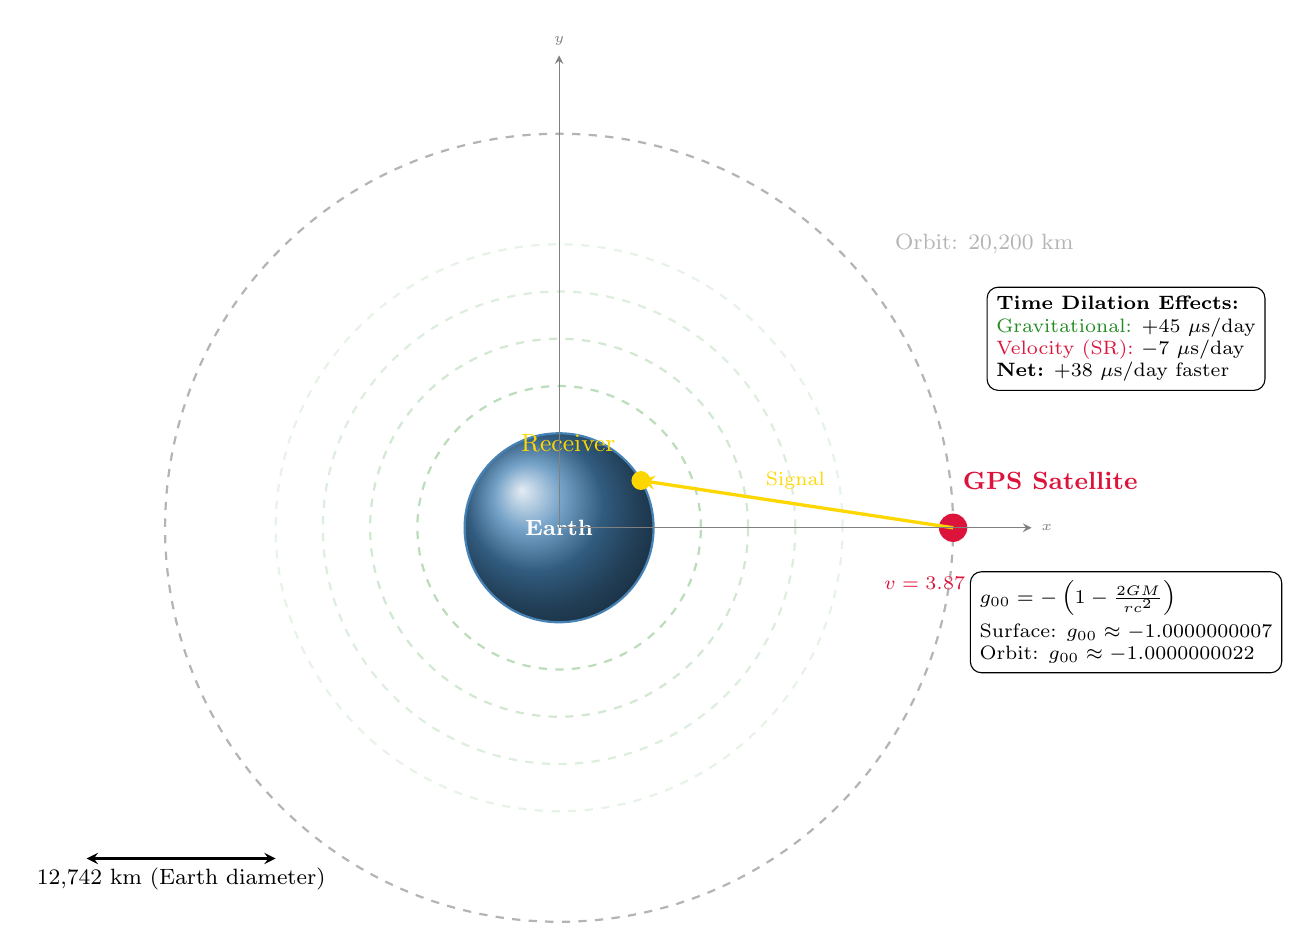
\begin{tikzpicture}[scale=1.2, >=stealth]
  
  % Define colors
  \definecolor{earthblue}{RGB}{70,130,180}
  \definecolor{orbitgray}{RGB}{180,180,180}
  \definecolor{satred}{RGB}{220,20,60}
  \definecolor{potentialgreen}{RGB}{34,139,34}
  \definecolor{signalgold}{RGB}{255,215,0}
  
  % Earth (radius normalized to 1 unit = 6371 km)
  \shade[ball color=earthblue] (0,0) circle (1);
  \draw[thick, earthblue] (0,0) circle (1);
  \node at (0,0) {\footnotesize \textcolor{white}{\textbf{Earth}}};
  
  % Gravitational potential contours
  \foreach \r/\opacity in {1.5/0.3, 2.0/0.2, 2.5/0.15, 3.0/0.1} {
    \draw[potentialgreen, opacity=\opacity, dashed, thick] (0,0) circle (\r);
  }
  
  % GPS orbit (altitude 20,200 km → radius 4.17 Earth radii)
  \draw[thick, orbitgray, dashed] (0,0) circle (4.17);
  \node[orbitgray] at (4.5, 3) {\footnotesize Orbit: 20,200 km};
  
  % GPS satellite
  \fill[satred] (4.17, 0) circle (0.15);
  \node[satred, above right] at (4.17, 0.3) {\small \textbf{GPS Satellite}};
  \node[satred, below] at (4.17, -0.4) {\scriptsize $v = 3.87$ km/s};
  
  % Ground receiver
  \fill[signalgold] (0.866, 0.5) circle (0.1);  % At 30° on surface
  \node[signalgold, above left] at (0.7, 0.7) {\small Receiver};
  
  % Signal path
  \draw[signalgold, very thick, ->] (4.17, 0) -- (0.866, 0.5);
  \node[signalgold] at (2.5, 0.5) {\scriptsize Signal};
  
  % Time dilation annotations
  \node[draw, fill=white, rounded corners, align=left, font=\scriptsize] at (6, 2) {
    \textbf{Time Dilation Effects:}\\
    \textcolor{potentialgreen}{Gravitational:} $+45$ $\mu$s/day\\
    \textcolor{satred}{Velocity (SR):} $-7$ $\mu$s/day\\
    \textbf{Net:} $+38$ $\mu$s/day faster
  };
  
  % Metric annotation
  \node[draw, fill=white, rounded corners, align=left, font=\scriptsize] at (6, -1) {
    $g_{00} = -\left(1 - \frac{2GM}{rc^2}\right)$\\[2pt]
    Surface: $g_{00} \approx -1.0000000007$\\
    Orbit: $g_{00} \approx -1.0000000022$
  };
  
  % Scale bar
  \draw[<->, thick] (-5, -3.5) -- (-3, -3.5);
  \node[below] at (-4, -3.5) {\footnotesize 12,742 km (Earth diameter)};
  
  % Coordinate axes
  \draw[->, gray] (0,0) -- (5, 0) node[right] {\tiny $x$};
  \draw[->, gray] (0,0) -- (0, 5) node[above] {\tiny $y$};
  
\end{tikzpicture}
\caption{GPS satellite orbit geometry showing gravitational time dilation effects. The satellite at 20,200 km altitude experiences weaker gravitational field (lighter green contours) than Earth's surface, causing its clock to run faster by $+45$ $\mu$s/day. Combined with special relativistic velocity time dilation ($-7$ $\mu$s/day), the net effect is $+38$ $\mu$s/day faster. Without correction, position errors accumulate at $\approx 11$ km/day, making Einstein's equations essential for navigation.}
\label{fig:prelim:gps-orbit-detailed}
\end{figure}

\caption{GPS satellite orbit geometry with gravitational potential contours. The satellite at altitude $h = \SI{20200}{\kilo\meter}$ experiences gravitational time dilation of $+\SI{45}{\micro\second}/\text{day}$ (clocks run faster) and velocity time dilation of $-\SI{7}{\micro\second}/\text{day}$ (clocks run slower), yielding net effect of $+\SI{38}{\micro\second}/\text{day}$. \mnote{GPS orbit: $r = \SI{26600}{\kilo\meter}$ from Earth center, $v = \SI{3.87}{\kilo\meter/\second}$ orbital velocity.}}
\label{fig:prelim:gps-orbit}
\end{figure}

\mphys{Without relativistic corrections, GPS positioning errors would accumulate at $\SI{11}{\kilo\meter}/\text{day}$, rendering the system useless within hours.}

% Time dilation budget: Comprehensive breakdown
% Table: GPS Time Dilation Budget
% Comprehensive breakdown of relativistic effects on GPS timing
% Lions Commentary style: exhaustive detail with physical interpretation

\begin{table}[htbp]
\centering
\caption{Comprehensive Time Dilation Budget for GPS Satellites}
\label{tab:prelim:gps-budget}
\begin{tabular}{llccp{5cm}}
\toprule
\textbf{Effect} & \textbf{Theory} & \textbf{Sign} & \textbf{Magnitude} & \textbf{Physical Cause} \\
& & & ($\mu$s/day) & \\
\midrule
\multicolumn{5}{l}{\textit{Gravitational Time Dilation (General Relativity)}} \\
\quad Surface potential & GR & Reference & 0 & $\Phi_{\text{surf}} = -62.6$ MJ/kg \\
\quad Orbit potential & GR & Faster & $+45.7$ & Weaker field: $\Phi_{\text{orbit}} = -52.3$ MJ/kg \\
\quad Net gravitational & GR & Faster & $+45.7$ & $\Delta\Phi = +10.3$ MJ/kg \\
\midrule
\multicolumn{5}{l}{\textit{Velocity Time Dilation (Special Relativity)}} \\
\quad Orbital velocity & SR & Slower & $-7.1$ & $v_{\text{orbit}} = 3.87$ km/s \\
\quad Factor & SR & — & — & $\gamma^{-1} \approx 1 - v^2/(2c^2)$ \\
\midrule
\multicolumn{5}{l}{\textit{Combined Relativistic Effects}} \\
\quad Net effect & GR+SR & Faster & $\mathbf{+38.6}$ & Measured value: $+38.4 \pm 0.1$ \\
\quad Daily error & — & Growth & $11.4$ km & Without correction \\
\quad Per-minute error & — & Growth & $7.9$ m & Navigation failure time \\
\midrule
\multicolumn{5}{l}{\textit{Dimensional Analysis}} \\
\quad Gravitational & — & — & $gh/c^2 \times (1$ day$)$ & $g = 9.8$ m/s$^2$, $h = 20{,}200$ km \\
\quad Velocity & — & — & $v^2/(2c^2) \times (1$ day$)$ & $v^2/c^2 \approx 1.66 \times 10^{-10}$ \\
\midrule
\multicolumn{5}{l}{\textit{Correction Implementation}} \\
\quad Frequency offset & Engineering & Pre-adjusted & $-4.465 \times 10^{-10}$ & Factory setting \\
\quad On-orbit tuning & Engineering & Real-time & $\pm 10^{-12}$ & Ground control \\
\quad Final accuracy & System & Achieved & $< 0.01$ $\mu$s & Sub-meter precision \\
\bottomrule
\end{tabular}
\end{table}

\begin{table}[htbp]
\centering
\caption{Comparison of Spacetime Curvature Effects Across Altitudes}
\label{tab:prelim:curvature-altitudes}
\begin{tabular}{lcccc}
\toprule
\textbf{Location} & \textbf{Altitude} & \textbf{$g_{00}$ Component} & \textbf{$\Delta t$/day} & \textbf{Position Error} \\
& (km) & & ($\mu$s) & (without correction) \\
\midrule
Earth Surface & 0 & $-1.0000000007$ & Reference & — \\
Commercial Aircraft & 10 & $-1.0000000008$ & $+0.1$ & $\sim 30$ m/day \\
Low Earth Orbit & 400 & $-1.0000000011$ & $+4.3$ & $\sim 1.3$ km/day \\
GPS Orbit & 20,200 & $-1.0000000022$ & $+38.6$ & $11.4$ km/day \\
Geostationary Orbit & 35,786 & $-1.0000000032$ & $+53.2$ & $15.7$ km/day \\
Moon & 384,400 & $-1.0000000125$ & $+125$ & $\sim 37$ km/day \\
\midrule
\multicolumn{5}{l}{\textit{Physical Interpretation:}} \\
\multicolumn{5}{p{13cm}}{The $g_{00}$ component of the metric tensor directly determines gravitational time dilation. Larger deviations from $-1$ (Minkowski value) indicate stronger time dilation effects. GPS satellites experience moderate time dilation, sufficient to require correction but weak enough for Newtonian approximation $g_{00} \approx -(1 + 2\Phi/c^2)$ to remain accurate.} \\
\bottomrule
\end{tabular}
\end{table}

\mdim{Gravitational time dilation scales as $\Delta t/t \approx GM/(rc^2) \approx 10^{-9}$ at GPS altitude. Velocity effect scales as $v^2/(2c^2) \approx 10^{-10}$.}

%-----------------------------------------------------------------------------
\section{Building Intuition: Why Curved Spacetime Requires a Metric}
\label{sec:prelim:motivation}
%-----------------------------------------------------------------------------

\subsection{The Failure of Flat-Space Geometry}

Consider measuring the sum of angles in a triangle. On a flat sheet of paper, Euclid proved this sum is always \SI{180}{\degree}. But draw a triangle on a sphere: connect the North Pole to two points on the equator separated by \SI{90}{\degree} of longitude.

This spherical triangle has three \SI{90}{\degree} angles---a total of \SI{270}{\degree}. The geometry is fundamentally different from Euclid's flat space. The ``straight'' lines (geodesics) are great circles, not the straight lines of a plane.

Now replace the sphere with spacetime near Earth. Just as the sphere's curvature distorts triangles, gravitational curvature distorts the paths of light, the flow of time, and the trajectories of satellites. We need mathematical machinery to quantify this curvature.

\subsection{Motivation for the Metric Tensor}

How do we measure distances in curved space? On a flat plane, the Pythagorean theorem gives the distance:
\begin{equation}
  ds^2 = dx^2 + dy^2 \quad \text{(flat Euclidean space)}
  \label{eq:prelim:euclidean}
\end{equation}

But on a sphere of radius $R$, the proper distance element is:
\begin{equation}
  ds^2 = R^2 \left( d\theta^2 + \sin^2\theta \, d\phi^2 \right) \quad \text{(curved spherical surface)}
  \label{eq:prelim:sphere}
\end{equation}

Notice the $\sin^2\theta$ factor---this encodes the curvature. Circles of latitude get smaller as you approach the poles. The geometry itself changes from point to point.

In spacetime, we need an even more general description. Near a massive object, not just space but \emph{time} is curved. The metric must account for both spatial distances and temporal intervals, mixing them in relativistic fashion.

This motivates the \textbf{metric tensor}\index{metric tensor}\index{tensor!metric} $g_{\mu\nu}$, which encodes both the geometry of spacetime and the gravitational field:

%==============================================================================
% Equation: Metric line element (spacetime interval)
% Source: Standard general relativity textbooks (MTW, Carroll, Wald)
% Provenance: Foundation for all frameworks - tensor calculus preliminaries
%==============================================================================
\begin{equation}
  \dd s^{2} = g_{\mu\nu} \, \dd x^{\mu} \dd x^{\nu}
  \eqtag{M}{MATH}{T}
  \label{eq:prelim:metric-line-element}
\end{equation}
% Notes:
%   * $g_{\mu\nu}$ is the spacetime metric tensor (rank-2 covariant tensor)
%   * $\dd x^{\mu}$ are coordinate differentials ($\mu = 0,1,2,3$ in 4D)
%   * $\dd s^2$ is the invariant spacetime interval
%   * Signature: $(-,+,+,+)$ (mostly plus convention)
%==============================================================================


\textbf{Physical interpretation of each element}:
\begin{itemize}
  \item $ds^2$: The \textbf{invariant spacetime interval}\index{spacetime interval}\index{proper time|see{spacetime interval}}---proper time for timelike paths, proper distance for spacelike paths. All observers agree on this quantity regardless of their motion.

  \item $g_{\mu\nu}$: The \textbf{metric tensor} encodes curvature. In flat Minkowski spacetime, $g_{\mu\nu} = \eta_{\mu\nu} = \text{diag}(-1,+1,+1,+1)$. Deviations from this diagonal form represent gravitational fields.

  \item $dx^\mu dx^\nu$: Infinitesimal coordinate displacements. The Einstein summation convention means we sum over all $\mu,\nu = 0,1,2,3$ (with repeated indices summed).

  \item \textbf{Signature} $(-,+,+,+)$: Time has opposite sign to space. This encodes causality: timelike intervals ($ds^2 < 0$) represent possible particle worldlines, while spacelike intervals ($ds^2 > 0$) cannot be traversed by any signal.
\end{itemize}

\mxref{See \S\ref{sec:prelim:curvature} for how metric determines curvature via Riemann tensor.}

%-----------------------------------------------------------------------------
% METRIC TENSOR: Structure Visualization
%-----------------------------------------------------------------------------

\begin{figure}[htbp]
\centering
% TikZ Diagram: Metric Tensor Components Visualization
% 4×4 matrix with physical interpretation of each element
% Pedagogical breakdown inspired by Lions Commentary annotation style

\begin{figure}[htbp]
\centering
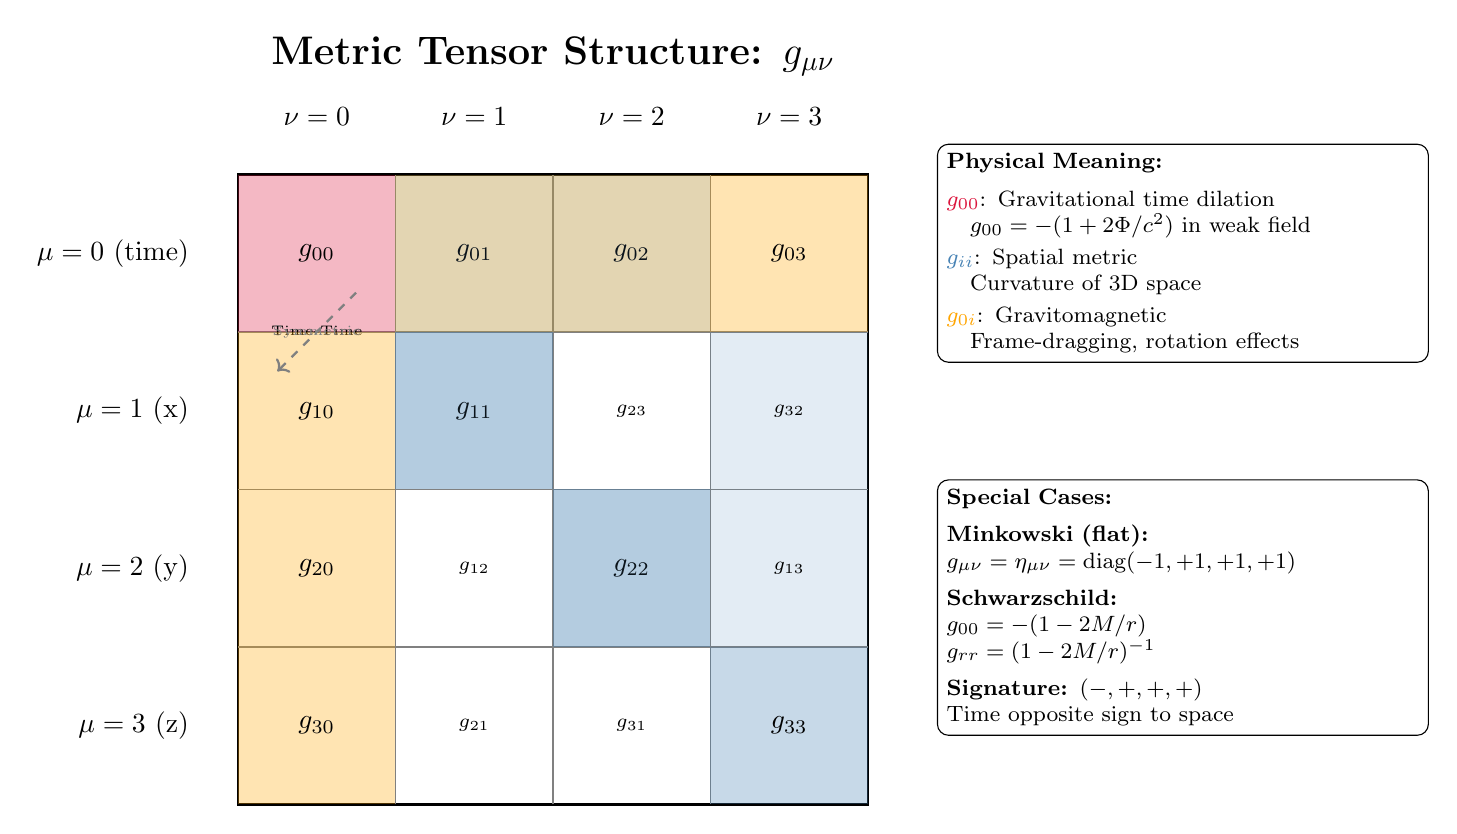
\begin{tikzpicture}[scale=1.0]
  
  % Define colors for different component types
  \definecolor{timecolor}{RGB}{220,20,60}      % Red for time-time
  \definecolor{spacecolor}{RGB}{70,130,180}    % Blue for space-space
  \definecolor{mixedcolor}{RGB}{255,165,0}     % Orange for time-space
  \definecolor{labelcolor}{RGB}{50,50,50}      % Dark gray for labels
  
  % Matrix outline
  \draw[thick] (0,0) rectangle (8,8);
  
  % Grid lines
  \foreach \i in {2,4,6} {
    \draw[gray] (0,\i) -- (8,\i);
    \draw[gray] (\i,0) -- (\i,8);
  }
  
  % g_00 component (time-time)
  \fill[timecolor, opacity=0.3] (0,6) rectangle (2,8);
  \node at (1,7) {$g_{00}$};
  \node[below, font=\tiny] at (1,6.2) {Time-Time};
  
  % g_0i components (time-space, off-diagonal)
  \fill[mixedcolor, opacity=0.3] (2,6) rectangle (4,8);
  \node at (3,7) {$g_{01}$};
  \fill[mixedcolor, opacity=0.3] (4,6) rectangle (6,8);
  \node at (5,7) {$g_{02}$};
  \fill[mixedcolor, opacity=0.3] (6,6) rectangle (8,8);
  \node at (7,7) {$g_{03}$};
  
  % g_i0 components (space-time, symmetric)
  \fill[mixedcolor, opacity=0.3] (0,4) rectangle (2,6);
  \node at (1,5) {$g_{10}$};
  \fill[mixedcolor, opacity=0.3] (0,2) rectangle (2,4);
  \node at (1,3) {$g_{20}$};
  \fill[mixedcolor, opacity=0.3] (0,0) rectangle (2,2);
  \node at (1,1) {$g_{30}$};
  
  % g_ij components (space-space, diagonal)
  \fill[spacecolor, opacity=0.3] (2,4) rectangle (4,6);
  \node at (3,5) {$g_{11}$};
  \fill[spacecolor, opacity=0.3] (4,2) rectangle (6,4);
  \node at (5,3) {$g_{22}$};
  \fill[spacecolor, opacity=0.3] (6,0) rectangle (8,2);
  \node at (7,1) {$g_{33}$};
  
  % Off-diagonal space-space components
  \foreach \i/\j in {2/4, 2/6, 4/6, 4/2, 6/2, 6/4} {
    \fill[spacecolor, opacity=0.15] (\i,\j) rectangle (\i+2,\j+2);
  }
  \node[font=\scriptsize] at (3,3) {$g_{12}$};
  \node[font=\scriptsize] at (5,5) {$g_{23}$};
  \node[font=\scriptsize] at (7,3) {$g_{13}$};
  \node[font=\scriptsize] at (3,1) {$g_{21}$};
  \node[font=\scriptsize] at (5,1) {$g_{31}$};
  \node[font=\scriptsize] at (7,5) {$g_{32}$};
  
  % Axis labels
  \node[left] at (-0.5,7) {$\mu=0$ (time)};
  \node[left] at (-0.5,5) {$\mu=1$ (x)};
  \node[left] at (-0.5,3) {$\mu=2$ (y)};
  \node[left] at (-0.5,1) {$\mu=3$ (z)};
  
  \node[above] at (1,8.5) {$\nu=0$};
  \node[above] at (3,8.5) {$\nu=1$};
  \node[above] at (5,8.5) {$\nu=2$};
  \node[above] at (7,8.5) {$\nu=3$};
  
  % Symmetry indicator
  \draw[->, thick, dashed, gray] (1.5,6.5) -- (0.5,5.5);
  \node[gray, font=\tiny] at (1,6) {Symmetric};
  
  % Physical interpretation annotations (right side)
  \node[draw, rounded corners, fill=white, align=left, font=\footnotesize, text width=6cm] at (12,7) {
    \textbf{Physical Meaning:}\\[4pt]
    \textcolor{timecolor}{\textbf{$g_{00}$}}: Gravitational time dilation\\
    \quad $g_{00} = -(1 + 2\Phi/c^2)$ in weak field\\[2pt]
    \textcolor{spacecolor}{\textbf{$g_{ii}$}}: Spatial metric\\
    \quad Curvature of 3D space\\[2pt]
    \textcolor{mixedcolor}{\textbf{$g_{0i}$}}: Gravitomagnetic\\
    \quad Frame-dragging, rotation effects
  };
  
  % Minkowski limit annotation (bottom right)
  \node[draw, rounded corners, fill=white, align=left, font=\footnotesize, text width=6cm] at (12,2.5) {
    \textbf{Special Cases:}\\[4pt]
    \textbf{Minkowski (flat):}\\
    $g_{\mu\nu} = \eta_{\mu\nu} = \text{diag}(-1,+1,+1,+1)$\\[4pt]
    \textbf{Schwarzschild:}\\
    $g_{00} = -(1-2M/r)$\\
    $g_{rr} = (1-2M/r)^{-1}$\\[4pt]
    \textbf{Signature:} $(-,+,+,+)$\\
    Time opposite sign to space
  };
  
  % Title
  \node[font=\Large\bfseries] at (4,9.5) {Metric Tensor Structure: $g_{\mu\nu}$};
  
\end{tikzpicture}
\caption{Structure of the metric tensor $g_{\mu\nu}$ showing the physical interpretation of each component. The \textcolor{timecolor}{red} element $g_{00}$ encodes gravitational time dilation, \textcolor{spacecolor}{blue} diagonal spatial elements $g_{ii}$ represent spatial curvature, and \textcolor{mixedcolor}{orange} off-diagonal $g_{0i}$ terms describe frame-dragging and rotation. The tensor is symmetric ($g_{\mu\nu} = g_{\nu\mu}$), reducing 16 components to 10 independent degrees of freedom. In flat Minkowski spacetime, all off-diagonal terms vanish and diagonal elements are $\pm 1$.}
\label{fig:prelim:metric-structure}
\end{figure}

\caption{Metric tensor $g_{\mu\nu}$ as a $4 \times 4$ symmetric matrix encoding spacetime geometry. Diagonal elements (red) represent time and space; off-diagonal terms (orange) indicate mixing. In flat Minkowski spacetime, $g_{\mu\nu} = \eta_{\mu\nu} = \text{diag}(-1,+1,+1,+1)$. Schwarzschild metric near Earth shows small deviations $\sim GM/(rc^2) \approx 10^{-9}$. \mphys{Signature $(-,+,+,+)$ encodes causality structure of spacetime.}}
\label{fig:prelim:metric-structure}
\end{figure}

\mdim{Metric is dimensionless. Line element $ds^2$ has dimensions $[\text{length}]^2$ or $[\text{time}]^2$ in natural units $c=1$.}

\subsection{Worked Example: Schwarzschild Metric Near Earth}

For GPS satellites, we need the metric in Earth's gravitational field. Outside a spherical mass $M$, the Schwarzschild solution\index{Schwarzschild metric}\index{metric!Schwarzschild} gives:
\begin{equation}
  ds^2 = -\left(1 - \frac{2GM}{rc^2}\right) c^2 dt^2 + \left(1 - \frac{2GM}{rc^2}\right)^{-1} dr^2 + r^2 d\Omega^2
  \label{eq:prelim:schwarzschild}
\end{equation}

For Earth, $GM/(rc^2) \approx 7 \times 10^{-10}$ at the surface. This is tiny, justifying a weak-field approximation:
\begin{equation}
  g_{00} \approx -\left(1 + \frac{2\Phi}{c^2}\right), \quad \Phi = -\frac{GM}{r}
  \label{eq:prelim:weak-field}
\end{equation}

The time component encodes gravitational time dilation. A clock at altitude $h$ ticks faster than a ground clock by:
\begin{equation}
  \frac{\Delta t_{\text{satellite}}}{\Delta t_{\text{ground}}} \approx 1 + \frac{GM}{c^2}\left(\frac{1}{R} - \frac{1}{R+h}\right) \approx 1 + \frac{gh}{c^2}
  \label{eq:prelim:time-dilation}
\end{equation}

For GPS at $h = \SI{20200}{\kilo\meter}$, $g = \SI{9.8}{\meter\per\second\squared}$:
\begin{equation}
  \frac{gh}{c^2} \approx \frac{9.8 \times 2.02 \times 10^7}{(3 \times 10^8)^2} \approx 2.2 \times 10^{-9}
  \label{eq:prelim:gps-number}
\end{equation}

Over one day ($\SI{86400}{\second}$), this produces:
\begin{equation}
  \Delta t \approx 86400 \times 2.2 \times 10^{-9} \approx \SI{1.9e-4}{\second} = \SI{190}{\micro\second}
  \label{eq:prelim:gps-day}
\end{equation}

Actually, special relativity's velocity time dilation ($v = \SI{3.87}{\kilo\meter\per\second}$) \emph{slows} the satellite clock by \SI{7}{\micro\second} per day. The net effect is approximately \SI{38}{\micro\second} per day faster, exactly as observed.

\textbf{Observable consequence}: Without correcting $g_{00}$ in the metric, GPS positioning drifts by \SI{11}{\kilo\meter} per day---about \SI{8}{\meter} per minute. Every navigation calculation implicitly solves Einstein's field equations.

\mcaution{Common misconception: Gravitational time dilation is not due to ``gravity slowing time.'' It's geometric---clocks measure intervals in curved spacetime, and $g_{00}$ quantifies the curvature.}

%-----------------------------------------------------------------------------
% LIGHT CONE STRUCTURE: Causality in Curved Spacetime
%-----------------------------------------------------------------------------

\begin{figure}[htbp]
\centering
% Light Cone Structure in Curved Spacetime
% Demonstrates tipping and deformation of light cones near massive objects
% Foundation for causal structure and event horizons

\begin{figure}[htbp]
\centering
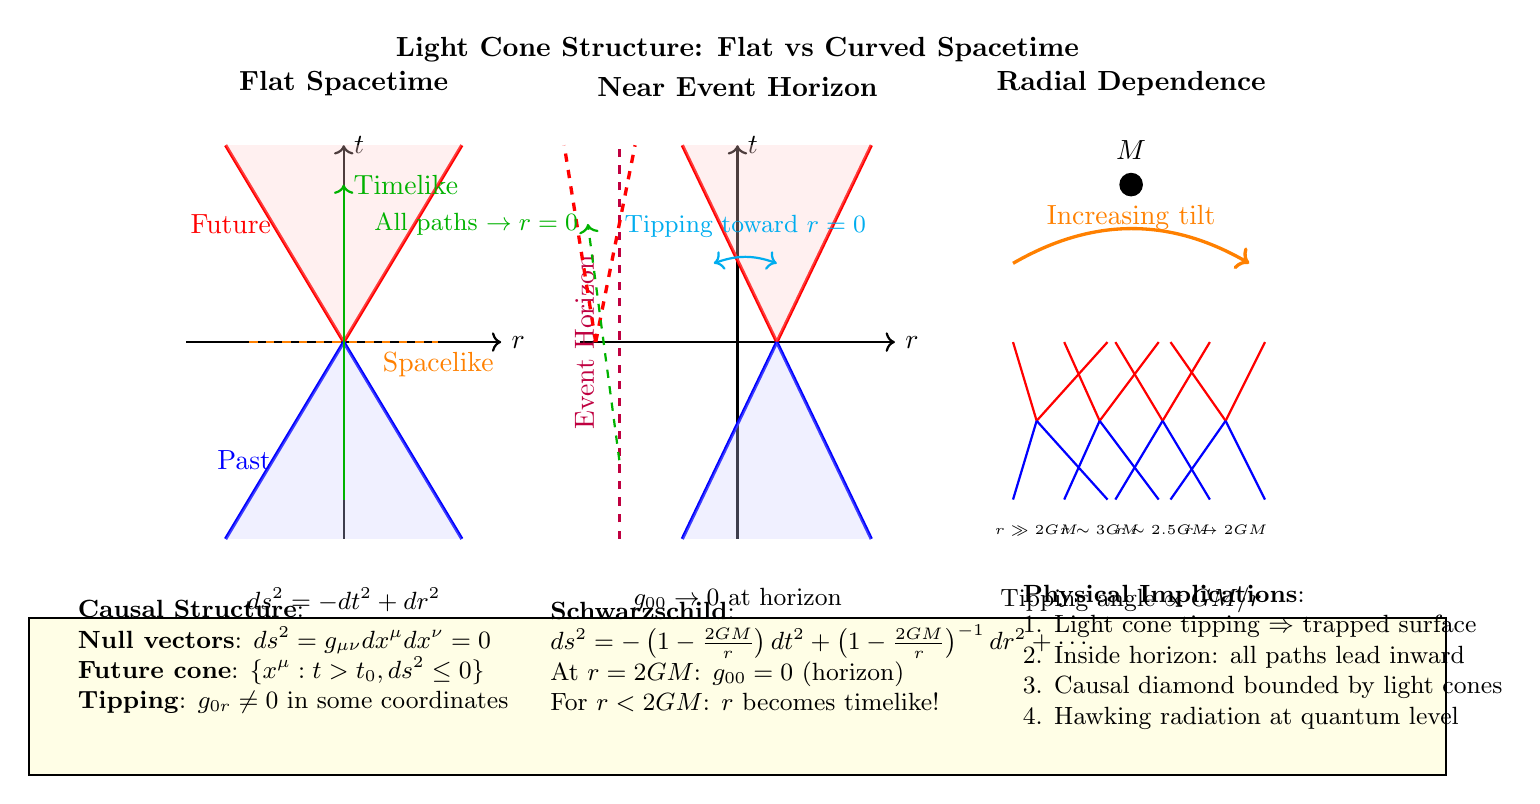
\begin{tikzpicture}[scale=1.0]
    % Title
    \node[anchor=north] at (0,6.5) {\textbf{Light Cone Structure: Flat vs Curved Spacetime}};
    
    % Left: Flat spacetime (Minkowski)
    \begin{scope}[xshift=-5cm]
        \node[above] at (0,5.5) {\textbf{Flat Spacetime}};
        
        % Axes
        \draw[->, thick] (0,0) -- (0,5) node[right] {$t$};
        \draw[->, thick] (-2,2.5) -- (2,2.5) node[right] {$r$};
        
        % Future light cone (symmetric)
        \draw[red, very thick] (0,2.5) -- (-1.5,5);
        \draw[red, very thick] (0,2.5) -- (1.5,5);
        \fill[red!20, opacity=0.3] (0,2.5) -- (-1.5,5) -- (1.5,5) -- cycle;
        
        % Past light cone (symmetric)
        \draw[blue, very thick] (0,2.5) -- (-1.5,0);
        \draw[blue, very thick] (0,2.5) -- (1.5,0);
        \fill[blue!20, opacity=0.3] (0,2.5) -- (-1.5,0) -- (1.5,0) -- cycle;
        
        % Time-like worldline
        \draw[->, green!70!black, thick] (0,0.5) -- (0,4.5);
        \node[green!70!black, right] at (0,4.5) {Timelike};
        
        % Space-like
        \draw[orange, thick, dashed] (-1.2,2.5) -- (1.2,2.5);
        \node[orange, below] at (1.2,2.5) {Spacelike};
        
        % Annotations
        \node[red, left] at (-0.8,4.0) {Future};
        \node[blue, left] at (-0.8,1.0) {Past};
        \node[below, align=center, font=\small] at (0,-0.5) {
            $ds^2 = -dt^2 + dr^2$\\
            Symmetric, unchanging
        };
    \end{scope}
    
    % Center: Schwarzschild near horizon
    \begin{scope}[xshift=0cm]
        \node[above] at (0,5.5) {\textbf{Near Event Horizon}};
        
        % Axes
        \draw[->, thick] (0,0) -- (0,5) node[right] {$t$};
        \draw[->, thick] (-2,2.5) -- (2,2.5) node[right] {$r$};
        
        % Event horizon (vertical dashed line)
        \draw[purple, very thick, dashed] (-1.5,0) -- (-1.5,5);
        \node[purple, above, rotate=90] at (-1.7,2.5) {Event Horizon};
        
        % Tipped light cone at r > 2GM
        \draw[red, very thick] (0.5,2.5) -- (-0.7,5);
        \draw[red, very thick] (0.5,2.5) -- (1.7,5);
        \fill[red!20, opacity=0.3] (0.5,2.5) -- (-0.7,5) -- (1.7,5) -- cycle;
        
        % Past cone (also tipped)
        \draw[blue, very thick] (0.5,2.5) -- (-0.7,0);
        \draw[blue, very thick] (0.5,2.5) -- (1.7,0);
        \fill[blue!20, opacity=0.3] (0.5,2.5) -- (-0.7,0) -- (1.7,0) -- cycle;
        
        % Tipping angle annotation
        \draw[<->, cyan, thick] (0.5,3.5) to[bend right=20] (-0.3,3.5);
        \node[cyan, above, font=\small] at (0.1,3.7) {Tipping toward $r=0$};
        
        % Inside horizon: light cones tip inward
        \draw[red, very thick, dashed] (-1.8,2.5) -- (-2.2,5);
        \draw[red, very thick, dashed] (-1.8,2.5) -- (-1.3,5);
        
        % Worldline forced inward
        \draw[->, green!70!black, thick, dashed] (-1.5,1.0) -- (-1.9,4.0);
        \node[green!70!black, left, font=\small] at (-1.9,4.0) {All paths $\to r=0$};
        
        \node[below, align=center, font=\small] at (0,-0.5) {
            $g_{00} \to 0$ at horizon\\
            Causal structure deformed
        };
    \end{scope}
    
    % Right: Strong field visualization
    \begin{scope}[xshift=5cm]
        \node[above] at (0,5.5) {\textbf{Radial Dependence}};
        
        % Multiple light cones at different radii
        \foreach \x/\tip in {-1.2/0.3, -0.4/0.15, 0.4/0.0, 1.2/-0.1} {
            \draw[red, thick] (\x,1.5) -- (\x-0.6+\tip,2.5);
            \draw[red, thick] (\x,1.5) -- (\x+0.6+\tip,2.5);
            \draw[blue, thick] (\x,1.5) -- (\x-0.6+\tip,0.5);
            \draw[blue, thick] (\x,1.5) -- (\x+0.6+\tip,0.5);
        }
        
        % Radial coordinate labels
        \node[below, font=\tiny] at (-1.2,0.3) {$r \gg 2GM$};
        \node[below, font=\tiny] at (-0.4,0.3) {$r \sim 3GM$};
        \node[below, font=\tiny] at (0.4,0.3) {$r \sim 2.5GM$};
        \node[below, font=\tiny] at (1.2,0.3) {$r \to 2GM$};
        
        % Tipping progression arrow
        \draw[->, orange, very thick] (-1.5,3.5) to[bend left=30] (1.5,3.5);
        \node[orange, above] at (0,3.8) {Increasing tilt};
        
        % Mass source
        \fill[black] (0,4.5) circle (0.15);
        \node[above] at (0,4.7) {$M$};
        
        \node[below, align=center, font=\small] at (0,-0.5) {
            Tipping angle $\propto GM/r$\\
            Causality preserved
        };
    \end{scope}
    
    % Bottom: Mathematical formulation
    \draw[thick, fill=yellow!10] (-9,-1.0) rectangle (9,-3.0);
    
    \node[align=left, font=\small, anchor=west] at (-8.5,-1.5) {
        \textbf{Causal Structure}:\\
        \textbf{Null vectors}: $ds^2 = g_{\mu\nu}dx^\mu dx^\nu = 0$\\
        \textbf{Future cone}: $\{x^\mu : t > t_0, ds^2 \leq 0\}$\\
        \textbf{Tipping}: $g_{0r} \neq 0$ in some coordinates
    };
    
    \node[align=left, font=\small, anchor=west] at (-2.5,-1.5) {
        \textbf{Schwarzschild}:\\
        $ds^2 = -\left(1-\frac{2GM}{r}\right)dt^2 + \left(1-\frac{2GM}{r}\right)^{-1}dr^2 + \cdots$\\
        At $r = 2GM$: $g_{00} = 0$ (horizon)\\
        For $r < 2GM$: $r$ becomes timelike!
    };
    
    \node[align=left, font=\small, anchor=west] at (3.5,-1.5) {
        \textbf{Physical Implications}:\\
        1. Light cone tipping $\Rightarrow$ trapped surface\\
        2. Inside horizon: all paths lead inward\\
        3. Causal diamond bounded by light cones\\
        4. Hawking radiation at quantum level
    };
    
\end{tikzpicture}
\caption{Light cone structure in curved spacetime. Left: flat Minkowski spacetime with symmetric light cones. Center: near Schwarzschild event horizon showing light cone tipping toward $r=0$, with all worldlines forced inward for $r < 2GM$. Right: radial progression showing increasing tilt as $r \to 2GM$. Bottom: mathematical formulation of causal structure and physical implications for black hole horizons.}
\label{fig:lightcone_curved}
\end{figure}

\caption{Light cone structure in flat Minkowski spacetime (left) versus curved Schwarzschild spacetime (right). Near a massive object, light cones tip progressively toward the event horizon, narrowing the causal future. At $r = 2GM/c^2$ (horizon), the light cone tips fully inward---nothing escapes. \mphys{Light cone tipping visualizes how gravity affects causality structure.}}
\label{fig:prelim:lightcone}
\end{figure}

\mxref{Light cone structure connects to geodesic equation in \S\ref{sec:prelim:geodesics}: photon paths follow null geodesics where $ds^2 = 0$.}

\subsection{Bridge to Covariant Derivatives}

The metric alone is not sufficient. We need to understand how vectors and tensors change as we move through curved spacetime. In flat space, a vector pointing ``north'' maintains its direction as you translate it. But on a sphere, ``north'' changes meaning as you move.

This requires introducing connection coefficients\index{connection coefficients|see{Christoffel symbols}} that encode how basis vectors rotate. This leads us to Christoffel symbols and covariant derivatives.

%-----------------------------------------------------------------------------
\section{Parallel Transport and Connection Coefficients}
\label{sec:prelim:connection}
%-----------------------------------------------------------------------------

\subsection{The Challenge of Comparing Vectors}

Here is a fundamental puzzle: \textbf{how do you compare vectors at different points in curved space?}

On a sphere, imagine walking along the equator from $(0^\circ, 0^\circ)$ to $(90^\circ \text{E}, 0^\circ)$ while holding a gyroscope pointed north. At the starting point, ``north'' means toward the North Pole. At $(90^\circ \text{E}, 0^\circ)$, ``north'' still means toward the North Pole, but the direction has changed in the ambient 3D space.

If you then walk north to the pole and back to the origin along the $0^\circ$ meridian, your gyroscope will be rotated by \SI{90}{\degree} relative to its starting orientation---even though you only walked along geodesics (great circles) and never ``turned'' the gyroscope yourself.

This rotation reveals curvature. The mathematical machinery that tracks how vectors change under transport is encoded in \textbf{Christoffel symbols}\index{Christoffel symbols}\index{parallel transport}.

\subsection{Christoffel Symbols: Encoding Geometry}

The Christoffel symbols (connection coefficients) of the Levi-Civita connection are defined by:

%==============================================================================
% Equation: Christoffel symbols (Levi-Civita connection)
% Source: Standard general relativity (Carroll, Wald, MTW)
% Provenance: Tensor calculus preliminaries
%==============================================================================
\begin{equation}
  \Gamma^{\lambda}_{\mu\nu} = \frac{1}{2} g^{\lambda\rho}
  \left( \partial_\mu g_{\nu\rho} + \partial_\nu g_{\rho\mu} - \partial_\rho g_{\mu\nu} \right)
  \eqtag{M}{MATH}{T}
  \label{eq:prelim:christoffel}
\end{equation}
% Notes:
%   * Christoffel symbols define the Levi-Civita connection (torsion-free, metric-compatible)
%   * Symmetric in lower indices: $\Gamma^{\lambda}_{\mu\nu} = \Gamma^{\lambda}_{\nu\mu}$
%   * Transform non-tensorially under coordinate changes
%   * Essential for covariant derivatives: $\nabla_\sigma V^\mu = \partial_\sigma V^\mu + \Gamma^\mu_{\sigma\rho} V^\rho$
%==============================================================================


Let's decode this formula term by term:

\begin{itemize}
  \item $\partial_\sigma g_{\mu\rho} = \partial g_{\mu\rho}/\partial x^\sigma$: How the metric changes as we move in the $\sigma$ direction. In flat space, the metric is constant, so these derivatives vanish.

  \item The symmetric combination $(\partial_\sigma g_{\mu\rho} + \partial_\mu g_{\rho\sigma} - \partial_\rho g_{\sigma\mu})$: This particular combination ensures the connection is \emph{metric-compatible}---parallel transport preserves lengths and angles.

  \item $g^{\nu\rho}$: The inverse metric tensor, used to raise indices. Satisfies $g^{\mu\rho} g_{\rho\nu} = \delta^\mu_\nu$.

  \item Factor of $1/2$: Emerges from demanding the connection is \emph{torsion-free}: $\Gamma^\rho_{\mu\nu} = \Gamma^\rho_{\nu\mu}$ (symmetric in lower indices).
\end{itemize}

\textbf{Physical meaning}: The Christoffel symbols tell you how much a vector component changes \emph{not} because the vector itself is changing, but because the coordinate basis vectors are rotating or stretching as you move.

\textbf{Units and dimensional analysis}: If coordinates $x^\mu$ have dimension $[L]$ and the metric is dimensionless (in geometric units), then $\Gamma^\rho_{\mu\nu}$ has dimension $[L^{-1}]$. For the Schwarzschild metric, $\Gamma^t_{tr} \sim GM/r^2 \sim g/c^2$ near Earth.

\mdim{Christoffel symbols $\Gamma^\rho_{\mu\nu}$ have dimension $[\text{length}]^{-1}$. For Earth, $\Gamma^t_{tr} \sim 10^{-17} \, \text{m}^{-1}$.}

%-----------------------------------------------------------------------------
% CHRISTOFFEL SYMBOLS: Computation Flowchart & Parallel Transport
%-----------------------------------------------------------------------------

\begin{figure}[htbp]
\centering
% Christoffel Symbol Computation Flowchart
% Pedagogical visualization showing step-by-step computation process
% For Chapter 1: Mathematical Preliminaries

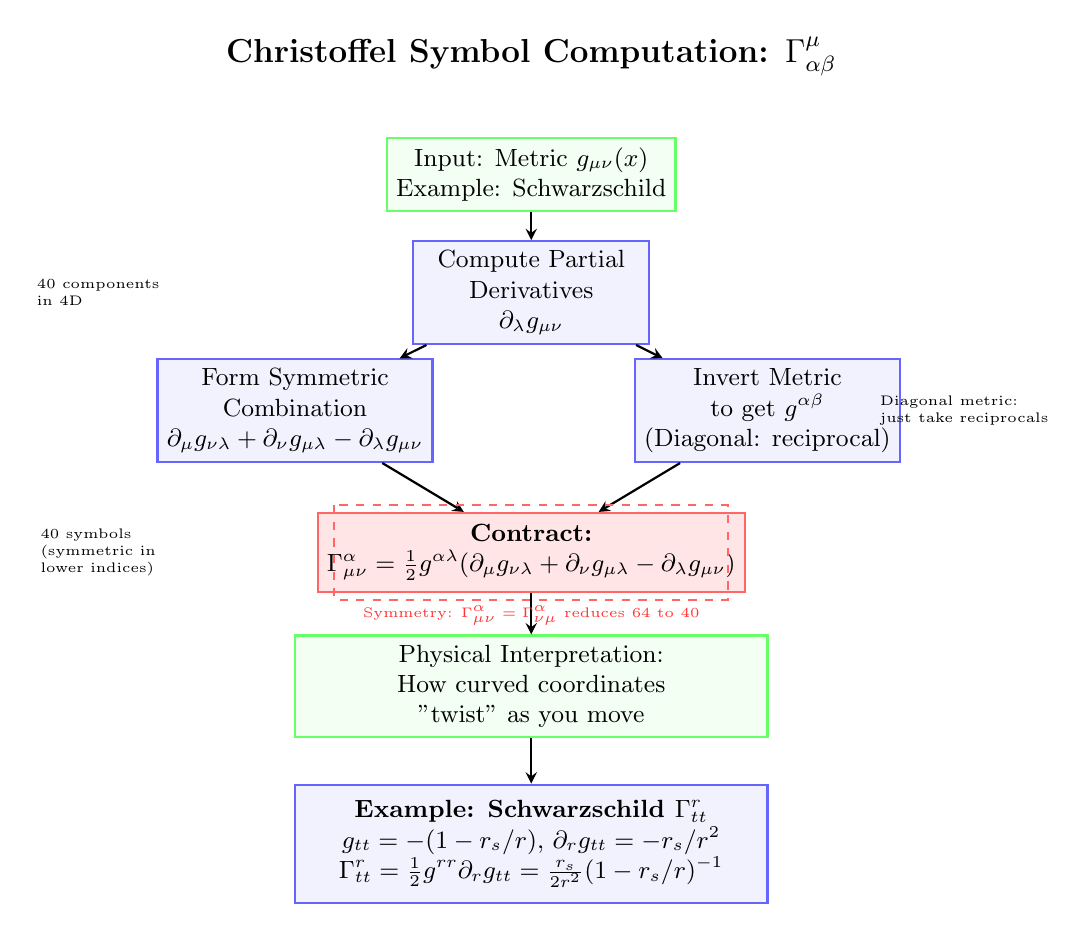
\begin{tikzpicture}[
    node distance=1.2cm and 2cm,
    box/.style={rectangle, draw=blue!60, fill=blue!5, thick, minimum width=3cm, minimum height=0.8cm, align=center, font=\small},
    databox/.style={rectangle, draw=green!60, fill=green!5, thick, minimum width=3cm, minimum height=0.8cm, align=center, font=\small},
    resultbox/.style={rectangle, draw=red!60, fill=red!10, thick, minimum width=3cm, minimum height=1cm, align=center, font=\small\bfseries},
    arrow/.style={->, >=stealth, thick}
]

% Title
\node[font=\large\bfseries] at (0,5.5) {Christoffel Symbol Computation: $\Gamma^\mu_{\alpha\beta}$};

% Step 1: Input metric
\node[databox] (metric) at (0,4) {Input: Metric $g_{\mu\nu}(x)$\\Example: Schwarzschild};

% Step 2: Compute derivatives
\node[box] (deriv) at (0,2.5) {Compute Partial\\Derivatives\\$\partial_\lambda g_{\mu\nu}$};

% Step 3: Form symmetric combination
\node[box] (symm) at (-3,1) {Form Symmetric\\Combination\\$\partial_\mu g_{\nu\lambda} + \partial_\nu g_{\mu\lambda} - \partial_\lambda g_{\mu\nu}$};

% Step 4: Invert metric
\node[box] (invert) at (3,1) {Invert Metric\\to get $g^{\alpha\beta}$\\(Diagonal: reciprocal)};

% Step 5: Contract
\node[resultbox] (result) at (0,-0.8) {Contract:\\$\Gamma^\alpha_{\mu\nu} = \frac{1}{2}g^{\alpha\lambda}(\partial_\mu g_{\nu\lambda} + \partial_\nu g_{\mu\lambda} - \partial_\lambda g_{\mu\nu})$};

% Step 6: Physical interpretation
\node[databox, minimum width=6cm] (phys) at (0,-2.5) {Physical Interpretation:\\How curved coordinates\\"twist" as you move};

% Example calculation box
\node[box, minimum width=6cm, minimum height=1.5cm] (example) at (0,-4.5) {
    \textbf{Example: Schwarzschild $\Gamma^r_{tt}$}\\
    $g_{tt} = -(1-r_s/r)$, $\partial_r g_{tt} = -r_s/r^2$\\
    $\Gamma^r_{tt} = \frac{1}{2}g^{rr}\partial_r g_{tt} = \frac{r_s}{2r^2}(1-r_s/r)^{-1}$
};

% Arrows
\draw[arrow] (metric) -- (deriv);
\draw[arrow] (deriv) -- (symm);
\draw[arrow] (deriv) -- (invert);
\draw[arrow] (symm) -- (result);
\draw[arrow] (invert) -- (result);
\draw[arrow] (result) -- (phys);
\draw[arrow] (phys) -- (example);

% Annotations
\node[font=\tiny, align=left] at (-5.5,2.5) {40 components\\in 4D};
\node[font=\tiny, align=left] at (5.5,1) {Diagonal metric:\\just take reciprocals};
\node[font=\tiny, align=left] at (-5.5,-0.8) {40 symbols\\(symmetric in\\lower indices)};

% Symmetry note
\draw[dashed, thick, red!60] (-2.5,-0.2) rectangle (2.5,-1.4);
\node[font=\tiny, text=red!80] at (0,-1.6) {Symmetry: $\Gamma^\alpha_{\mu\nu} = \Gamma^\alpha_{\nu\mu}$ reduces 64 to 40};

\end{tikzpicture}

\caption{Computational flowchart for Christoffel symbols: (1) Start with metric $g_{\mu\nu}$, (2) Compute partial derivatives $\partial_\sigma g_{\mu\rho}$, (3) Form symmetric combination, (4) Contract with inverse metric $g^{\nu\rho}$. Algorithm complexity: $O(D^4)$ for $D$ dimensions. \mcomp{Use symbolic computation (Mathematica, SymPy) for complex metrics.}}
\label{fig:prelim:christoffel-algo}
\end{figure}

\begin{figure}[htbp]
\centering
% Parallel Transport on a Sphere
% Demonstrates geometric meaning of covariant derivative
% Shows path-dependence of parallel transport in curved space

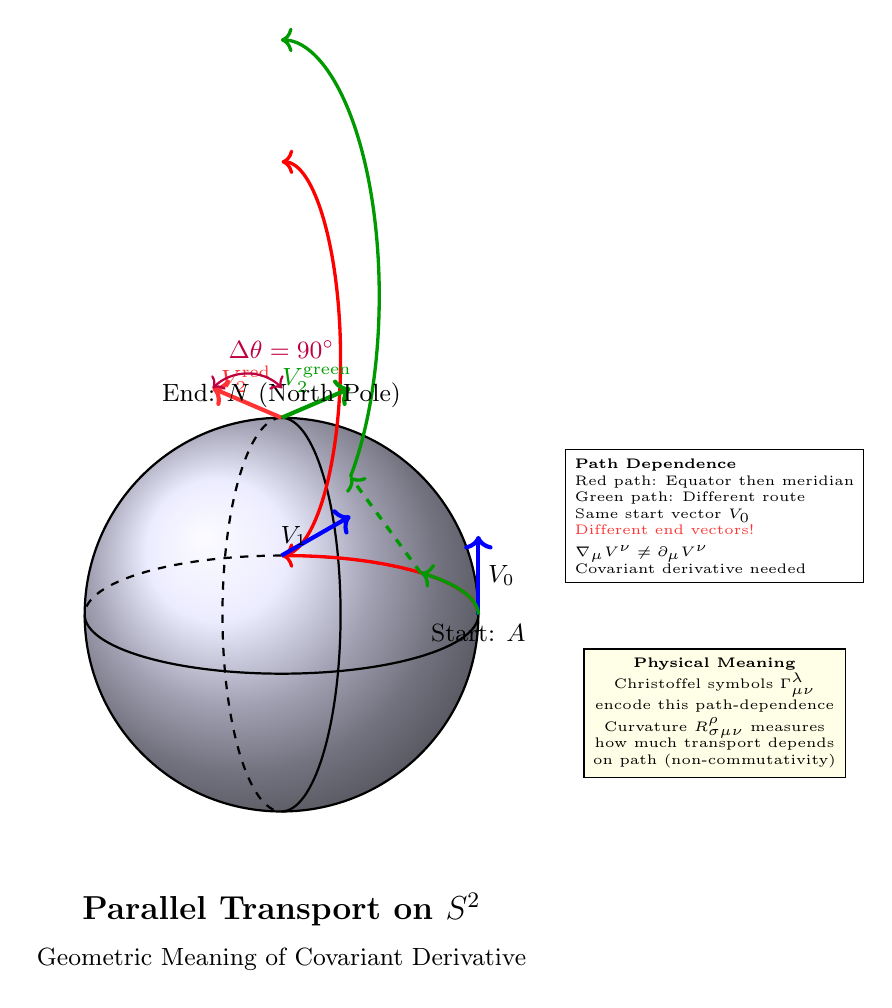
\begin{tikzpicture}[scale=2.5]

% Draw sphere
\shade[ball color=blue!10] (0,0) circle (1cm);
\draw[thick] (0,0) circle (1cm);

% Draw equator
\draw[thick, dashed] (1,0) arc (0:180:1 and 0.3);
\draw[thick] (-1,0) arc (180:360:1 and 0.3);

% Draw meridians
\draw[thick, dashed] (0,1) arc (90:270:0.3 and 1);
\draw[thick] (0,-1) arc (270:450:0.3 and 1);

% Path 1: Equator then meridian (red path)
\coordinate (A) at (1,0);
\coordinate (B) at (0,0.3);
\coordinate (C) at (0,1);

\draw[->, very thick, red] (A) arc (0:90:1 and 0.3);
\draw[->, very thick, red] (B) arc (-90:90:0.3 and 1);

% Vector at start (pointing north)
\draw[->, very thick, blue, line width=1.5pt] (1,0) -- (1,0.4);
\node[right, font=\small] at (1,0.2) {$V_0$};

% Vector after equator transport (still pointing north)
\draw[->, very thick, blue, line width=1.5pt] (0,0.3) -- (0.35,0.5);
\node[left, font=\small] at (0.18,0.4) {$V_1$};

% Vector at north pole after meridian transport (rotated!)
\draw[->, very thick, red!80, line width=1.5pt] (0,1) -- (-0.35,1.15);
\node[above, font=\small, text=red!80] at (-0.18,1.08) {$V_2^\text{red}$};

% Path 2: Different route (green path)
\draw[->, very thick, green!60!black] (A) arc (0:45:1 and 0.3);
\draw[->, very thick, green!60!black, dashed] (0.707,0.212) -- (0.35,0.7);
\draw[->, very thick, green!60!black] (0.35,0.7) arc (-45:90:0.5 and 1.3);

% Vector at north pole via green path (different rotation!)
\draw[->, very thick, green!60!black, line width=1.5pt] (0,1) -- (0.35,1.15);
\node[above, font=\small, text=green!60!black] at (0.18,1.08) {$V_2^\text{green}$};

% Labels
\node[below, font=\small] at (1,0) {Start: $A$};
\node[above, font=\small] at (0,1) {End: $N$ (North Pole)};

% Angle annotation
\draw[<->, thick, purple] (-0.35,1.15) arc (135:45:0.25);
\node[above, font=\small, text=purple] at (0,1.25) {$\Delta\theta = 90^\circ$};

% Legend box
\node[draw, fill=white, align=left, font=\tiny] at (2.2,0.5) {
    \textbf{Path Dependence}\\
    Red path: Equator then meridian\\
    Green path: Different route\\
    Same start vector $V_0$\\
    \textcolor{red!80}{Different end vectors!}\\[2pt]
    $\nabla_\mu V^\nu \neq \partial_\mu V^\nu$\\
    Covariant derivative needed
};

% Physical interpretation
\node[draw, fill=yellow!10, align=center, font=\tiny] at (2.2,-0.5) {
    \textbf{Physical Meaning}\\
    Christoffel symbols $\Gamma^\lambda_{\mu\nu}$\\
    encode this path-dependence\\[2pt]
    Curvature $R^\rho_{\sigma\mu\nu}$ measures\\
    how much transport depends\\
    on path (non-commutativity)
};

% Title
\node[font=\large\bfseries] at (0,-1.5) {Parallel Transport on $S^2$};
\node[font=\small] at (0,-1.75) {Geometric Meaning of Covariant Derivative};

\end{tikzpicture}

\caption{Parallel transport on a 2-sphere: Transport a vector (blue arrow) along two different paths from equator to North Pole. Path A: north along prime meridian. Path B: east along equator to $90^\circ$, then north. Final vectors differ by $90^\circ$ rotation. \mphys{Holonomy (path-dependence) measures curvature: flat space has zero holonomy.}}
\label{fig:prelim:parallel-transport}
\end{figure}

\mcaution{Parallel transport is \emph{path-dependent} in curved space. This is the geometric essence of curvature!}

\subsection{Worked Example: Christoffel Symbols for Schwarzschild Metric}

For the weak-field Schwarzschild metric equation~\eqref{eq:prelim:weak-field}, the key Christoffel symbol is:
\begin{equation}
  \Gamma^t_{tr} = \frac{1}{2} g^{tt} \partial_r g_{tt} = \frac{1}{2} \left(-1 - \frac{2\Phi}{c^2}\right)^{-1} \frac{\partial}{\partial r}\left[-1 - \frac{2\Phi}{c^2}\right]
  \label{eq:prelim:gamma-example}
\end{equation}

With $\Phi = -GM/r$:
\begin{equation}
  \Gamma^t_{tr} \approx -\frac{1}{c^2} \frac{\partial \Phi}{\partial r} = -\frac{1}{c^2} \frac{GM}{r^2} \approx \frac{g}{c^2}
  \label{eq:prelim:gamma-result}
\end{equation}

This single component generates:
\begin{itemize}
  \item \textbf{Gravitational redshift}: Photons climbing out of a gravitational well lose energy proportional to $\Phi$.
  \item \textbf{Gravitational time dilation}: Clocks tick slower deeper in the potential.
  \item \textbf{Geodesic deviation}: Free-falling objects converge toward the mass.
\end{itemize}

At Earth's surface, $\Gamma^t_{tr} \approx 9.8/(3 \times 10^8)^2 \approx 10^{-16}~\text{m}^{-1}$. Tiny---but measurable by atomic clocks and essential for GPS.

\subsection{Covariant Derivative: Taking Derivatives in Curved Space}

Ordinary partial derivatives do not respect the geometry. Taking $\partial_\mu V^\nu$ mixes changes in the vector $V^\nu$ with changes in the basis vectors. The \textbf{covariant derivative}\index{covariant derivative}\index{derivative!covariant} corrects for this:

%==============================================================================
% Equation: Covariant derivative of a contravariant vector
% Source: Standard differential geometry (Carroll Ch. 3, Wald Ch. 3)
% Provenance: Tensor calculus preliminaries
%==============================================================================
\begin{equation}
  \nabla_\sigma V^\mu = \partial_\sigma V^\mu + \Gamma^\mu_{\sigma\rho} V^\rho
  \eqtag{M}{MATH}{T}
  \label{eq:prelim:covariant-derivative-vector}
\end{equation}
% Notes:
%   * $\nabla_\sigma$ is the covariant derivative operator
%   * Transforms tensorially (unlike ordinary derivative $\partial_\sigma$)
%   * For covariant vectors: $\nabla_\sigma W_\mu = \partial_\sigma W_\mu - \Gamma^\rho_{\sigma\mu} W_\rho$
%   * Generalizes to arbitrary tensors by applying Leibniz rule
%   * Metric compatibility: $\nabla_\sigma g_{\mu\nu} = 0$
%==============================================================================


\textbf{Interpretation}:
\begin{itemize}
  \item $\partial_\sigma V^\mu$: Ordinary derivative of the vector components.
  \item $+\Gamma^\mu_{\nu\sigma} V^\nu$: Correction for how the basis vector $\mathbf{e}_\mu$ changes in the $\sigma$ direction.
\end{itemize}

For a covariant (lower-index) vector $W_\mu$, the signs flip:
\begin{equation}
  \nabla_\sigma W_\mu = \partial_\sigma W_\mu - \Gamma^\rho_{\sigma\mu} W_\rho
  \label{eq:prelim:covariant-lower}
\end{equation}

\textbf{Key property}: The metric tensor itself is covariantly constant:
\begin{equation}
  \nabla_\sigma g_{\mu\nu} = 0
  \label{eq:prelim:metric-covariant-constant}
\end{equation}

This is the defining property of the Levi-Civita connection: it preserves the metric under parallel transport.

\textbf{Limiting case}: In flat Minkowski spacetime with Cartesian coordinates, all $\Gamma^\mu_{\nu\sigma} = 0$, and the covariant derivative reduces to the ordinary partial derivative: $\nabla_\mu = \partial_\mu$.

\mxref{Covariant derivative generalizes to tensors: $\nabla_\sigma T^{\mu\nu} = \partial_\sigma T^{\mu\nu} + \Gamma^\mu_{\rho\sigma} T^{\rho\nu} + \Gamma^\nu_{\rho\sigma} T^{\mu\rho}$. One $\Gamma$ term per index.}

%-----------------------------------------------------------------------------
% COVARIANT VS ORDINARY DERIVATIVES: Comprehensive Comparison
%-----------------------------------------------------------------------------

% Comparison Table: Ordinary vs. Covariant Derivatives
% Pedagogical reference for understanding geometric derivatives

\begin{table}[htbp]
\centering
\caption{Ordinary Derivative vs. Covariant Derivative: Complete Comparison}
\label{tab:covariant_vs_ordinary}
\begin{tabular}{|l|c|c|p{4cm}|}
\hline
\rowcolor{gray!20}
\textbf{Property} & \textbf{Ordinary $\partial_\mu$} & \textbf{Covariant $\nabla_\mu$} & \textbf{Physical Interpretation} \\
\hline
\hline
\multicolumn{4}{|c|}{\cellcolor{blue!10}\textbf{Definition}} \\
\hline
Scalar field $\phi$ & $\partial_\mu\phi$ & $\nabla_\mu\phi = \partial_\mu\phi$ & Scalars: No difference \\
\hline
Vector field $V^\nu$ & $\partial_\mu V^\nu$ & $\nabla_\mu V^\nu = \partial_\mu V^\nu + \Gamma^\nu_{\mu\lambda}V^\lambda$ & Connection term corrects for basis change \\
\hline
Covector $\omega_\nu$ & $\partial_\mu\omega_\nu$ & $\nabla_\mu\omega_\nu = \partial_\mu\omega_\nu - \Gamma^\lambda_{\mu\nu}\omega_\lambda$ & Minus sign for lower index \\
\hline
\hline
\multicolumn{4}{|c|}{\cellcolor{green!10}\textbf{Transformation Properties}} \\
\hline
Under coord change & NOT tensorial & IS a tensor & $\nabla_\mu V^\nu$ transforms as $(0,1)+(1,1)=(1,2)$ tensor \\
\hline
Reason & $\partial_\mu$ derivatives transform & Christoffel terms cancel & Connection compensates non-tensorial part \\
\hline
\hline
\multicolumn{4}{|c|}{\cellcolor{yellow!10}\textbf{Geometric Meaning}} \\
\hline
What it measures & Component change in coords & Intrinsic geometric change & Moving through curved geometry \\
\hline
Flat space & Same as covariant & Same as ordinary & $\Gamma^\lambda_{\mu\nu} = 0$ in Cartesian \\
\hline
Curved space & Coord-dependent & Geometric invariant & Parallel transport encoded \\
\hline
\hline
\multicolumn{4}{|c|}{\cellcolor{red!10}\textbf{Metric Compatibility}} \\
\hline
$\partial_\mu g_{\alpha\beta}$ & Generally $\neq 0$ & $\nabla_\mu g_{\alpha\beta} = 0$ & Metric is covariantly constant \\
\hline
Physical meaning & Coords may be non-orthogonal & Lengths preserved under transport & Fundamental assumption of GR \\
\hline
\hline
\multicolumn{4}{|c|}{\cellcolor{purple!10}\textbf{Commutativity}} \\
\hline
$[\partial_\mu,\partial_\nu]\phi$ & Always $= 0$ & Always $= 0$ & Scalars commute \\
\hline
$[\nabla_\mu,\nabla_\nu]V^\rho$ & N/A & $= R^\rho_{\sigma\mu\nu}V^\sigma$ & Riemann tensor measures non-commutativity \\
\hline
Physical meaning & Flat space & Curvature & Path-dependence of parallel transport \\
\hline
\hline
\multicolumn{4}{|c|}{\cellcolor{orange!10}\textbf{Examples: Schwarzschild Metric}} \\
\hline
Radial component & $\partial_r V^t$ & $\nabla_r V^t = \partial_r V^t + \Gamma^t_{r\lambda}V^\lambda$ & $\Gamma^t_{rt} = \frac{r_s}{2r(r-r_s)}$ \\
\hline
Time component & $\partial_t V^r$ & $\nabla_t V^r = \partial_t V^r + \Gamma^r_{tt}V^t$ & $\Gamma^r_{tt} = \frac{r_s(r-r_s)}{2r^3}$ \\
\hline
\hline
\multicolumn{4}{|c|}{\cellcolor{cyan!10}\textbf{Computational Notes}} \\
\hline
Complexity & Simple: just differentiate & 40 Christoffel symbols needed & Symbolic computation helpful \\
\hline
For diagonal metric & Still simple & Simplifies: $\Gamma^i_{jk} = 0$ if $i \neq j \neq k$ & Many terms vanish \\
\hline
Numerical methods & Standard finite differences & Need connection interpolation & Geodesic integrators \\
\hline
\end{tabular}
\end{table}

% Second table: Index rules
\begin{table}[htbp]
\centering
\caption{Christoffel Symbol: Index Position Rules}
\label{tab:christoffel_index_rules}
\begin{tabular}{|l|c|l|}
\hline
\rowcolor{gray!20}
\textbf{Symbol Type} & \textbf{Index Pattern} & \textbf{Rule} \\
\hline
\hline
Upper index & $\Gamma^\lambda_{\mu\nu}$ & Raised by metric: $g^{\lambda\rho}\Gamma_{\rho,\mu\nu}$ \\
\hline
Lower indices & $\Gamma^\lambda_{\mu\nu}$ & Symmetric: $\Gamma^\lambda_{\mu\nu} = \Gamma^\lambda_{\nu\mu}$ \\
\hline
All lower & $\Gamma_{\lambda,\mu\nu}$ & $= \frac{1}{2}(\partial_\mu g_{\nu\lambda} + \partial_\nu g_{\mu\lambda} - \partial_\lambda g_{\mu\nu})$ \\
\hline
Count in 4D & 40 independent & $\binom{4+2-1}{2} \times 4 = 10 \times 4$ \\
\hline
Vanish when & Flat Cartesian coords & $\partial_\mu g_{\nu\lambda} = 0$ everywhere \\
\hline
Physical units & $[\text{length}]^{-1}$ & Inverse length scale of curvature \\
\hline
\end{tabular}
\end{table}


\mdim{Covariant derivative $\nabla_\mu$ and ordinary derivative $\partial_\mu$ have same dimensions $[\text{length}]^{-1}$. Difference is $\Gamma^\mu_{\nu\sigma} V^\nu$ with dimensions $[\text{length}]^{-1} \times [\text{vector}]$.}

\mcaution{Never use ordinary derivatives $\partial_\mu$ on tensor equations in curved spacetime! Always use covariant derivatives $\nabla_\mu$ to maintain geometric meaning.}

\subsection{Bridge to Curvature}

The Christoffel symbols tell us how vectors change under transport, but they do not directly reveal curvature. A clever choice of coordinates can make $\Gamma^\rho_{\mu\nu} = 0$ at any single point, even in curved space.

True curvature is detected by \emph{non-commutativity} of covariant derivatives. When you transport a vector around a closed loop, it returns rotated. The amount of rotation measures curvature. This is encoded in the Riemann curvature tensor\index{Riemann curvature tensor}\index{curvature!Riemann}.

%-----------------------------------------------------------------------------
\section{Curvature: When Derivatives Do Not Commute}
\label{sec:prelim:curvature}
%-----------------------------------------------------------------------------

\subsection{The Conceptual Meaning of Curvature}

Imagine transporting a vector around a small parallelogram in curved space:
\begin{enumerate}
  \item Start at point $P$ with vector $V$.
  \item Transport $V$ along direction $\mu$ by distance $\delta x^\mu$.
  \item Transport along direction $\nu$ by distance $\delta x^\nu$.
  \item Transport back in direction $-\mu$ by $\delta x^\mu$.
  \item Transport back in direction $-\nu$ by $\delta x^\nu$.
\end{enumerate}

In flat space, you return to the starting point with $V$ unchanged. In curved space, $V$ is rotated by an amount proportional to the area of the parallelogram. The proportionality factor is the Riemann curvature tensor.

\subsection{Riemann Tensor: Quantifying Curvature}

The Riemann curvature tensor measures the failure of covariant derivatives to commute:

%==============================================================================
% Equation: Riemann curvature tensor
% Source: Standard general relativity (MTW Box 11.4, Carroll Eq. 3.102, Wald Eq. 3.2.16)
% Provenance: Tensor calculus preliminaries
%==============================================================================
\begin{equation}
  R^\rho{}_{\sigma\mu\nu} = \partial_\mu \Gamma^\rho_{\nu\sigma}
  - \partial_\nu \Gamma^\rho_{\mu\sigma}
  + \Gamma^\rho_{\mu\lambda} \Gamma^\lambda_{\nu\sigma}
  - \Gamma^\rho_{\nu\lambda} \Gamma^\lambda_{\mu\sigma}
  \eqtag{M}{MATH}{T}
  \label{eq:prelim:riemann-curvature-tensor}
\end{equation}
% Notes:
%   * Measures non-commutativity of covariant derivatives: $[\nabla_\mu, \nabla_\nu] V^\rho = R^\rho{}_{\sigma\mu\nu} V^\sigma$
%   * Antisymmetric in last two indices: $R^\rho{}_{\sigma\mu\nu} = -R^\rho{}_{\sigma\nu\mu}$
%   * Satisfies Bianchi identity: $R_{\rho[\sigma\mu\nu]} = 0$ (cyclic sum)
%   * Vanishes in flat spacetime
%   * Ricci tensor: $R_{\mu\nu} = R^\rho{}_{\mu\rho\nu}$
%   * Ricci scalar: $R = g^{\mu\nu} R_{\mu\nu}$
%==============================================================================


\textbf{Unpacking this definition}:
\begin{itemize}
  \item $[\nabla_\mu, \nabla_\nu] V^\rho \equiv \nabla_\mu \nabla_\nu V^\rho - \nabla_\nu \nabla_\mu V^\rho$: The commutator of covariant derivatives acting on a vector.

  \item $R^\rho{}_{\sigma\mu\nu} V^\sigma$: The result is proportional to the original vector. The Riemann tensor is the proportionality factor.

  \item \textbf{Four indices}: Two ($\mu, \nu$) specify the directions of the loop. One ($\sigma$) is the component of the vector being transported. One ($\rho$) is the component of the result.
\end{itemize}

With our conventions (mostly plus signature), the explicit formula is:
\begin{equation}
  R^\rho{}_{\sigma\mu\nu} = \partial_\mu \Gamma^\rho_{\nu\sigma} - \partial_\nu \Gamma^\rho_{\mu\sigma} + \Gamma^\rho_{\mu\lambda} \Gamma^\lambda_{\nu\sigma} - \Gamma^\rho_{\nu\lambda} \Gamma^\lambda_{\mu\sigma}
  \label{eq:prelim:riemann-explicit}
\end{equation}

\textbf{Symmetries} (essential for understanding curvature):
\begin{align}
  R^\rho{}_{\sigma\mu\nu} &= -R^\rho{}_{\sigma\nu\mu} \quad \text{(antisymmetric in last two indices)} \label{eq:prelim:riemann-antisym1} \\
  R_{\rho\sigma\mu\nu} &= R_{\mu\nu\rho\sigma} \quad \text{(symmetric in first and last pairs)} \label{eq:prelim:riemann-sym} \\
  R_{\rho\sigma\mu\nu} + R_{\rho\mu\nu\sigma} + R_{\rho\nu\sigma\mu} &= 0 \quad \text{(first Bianchi identity)} \label{eq:prelim:bianchi}
\end{align}

These symmetries reduce the 256 components of $R^\rho{}_{\sigma\mu\nu}$ in 4D to just 20 independent components.

\mcomp{Computing Riemann tensor: $O(D^5)$ operations for $D$ dimensions. For Schwarzschild metric: $R_{trtr} \sim (GM/r^3)$ (tidal term).}

%-----------------------------------------------------------------------------
% RIEMANN TENSOR: Holonomy & Comprehensive Properties
%-----------------------------------------------------------------------------

\begin{figure}[htbp]
\centering
% Riemann Tensor: Geometric Meaning via Parallel Transport Loop
% Shows how curvature manifests as rotation after closed path

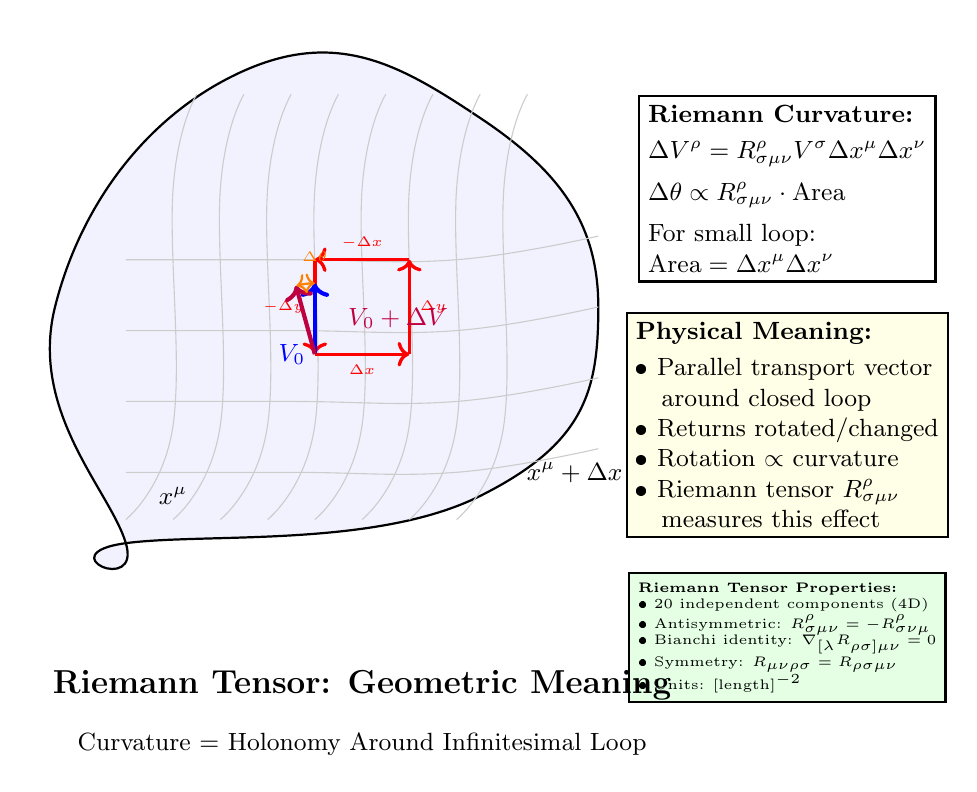
\begin{tikzpicture}[scale=3]

% Draw curved surface (2D projection of curved space)
\draw[thick, fill=blue!5] plot[smooth cycle, tension=0.8] coordinates {
    (0,0) (1.5,0.2) (2,1) (1.5,1.8) (0.5,2) (-0.3,1) (0,0)
};

% Grid on surface to show curvature
\foreach \x in {0.2,0.4,...,1.6} {
    \draw[gray!40, thin] plot[smooth, tension=0.7] coordinates {
        (\x-0.2,0.1) (\x,0.5) (\x,1.5) (\x+0.1,1.9)
    };
}
\foreach \y in {0.3,0.6,...,1.5} {
    \draw[gray!40, thin] plot[smooth, tension=0.7] coordinates {
        (0,\y) (0.7,\y) (1.4,\y) (2,\y+0.1)
    };
}

% Closed path (small loop)
\coordinate (P1) at (0.8,0.8);
\coordinate (P2) at (1.2,0.8);
\coordinate (P3) at (1.2,1.2);
\coordinate (P4) at (0.8,1.2);

% Draw the loop with directional arrows
\draw[->, very thick, red] (P1) -- node[below, font=\tiny] {$\Delta x$} (P2);
\draw[->, very thick, red] (P2) -- node[right, font=\tiny] {$\Delta y$} (P3);
\draw[->, very thick, red] (P3) -- node[above, font=\tiny] {$-\Delta x$} (P4);
\draw[->, very thick, red] (P4) -- node[left, font=\tiny] {$-\Delta y$} (P1);

% Vector at start
\draw[->, very thick, blue, line width=1.5pt] (P1) -- ++(0,0.3);
\node[left, font=\small, text=blue] at (P1) {$V_0$};

% Vector after loop (rotated slightly due to curvature)
\draw[->, very thick, purple, line width=1.5pt] (P1) -- ++(-0.08,0.29);
\node[right, font=\small, text=purple] at ($(P1)+(0.1,0.15)$) {$V_0 + \Delta V$};

% Rotation angle annotation
\draw[<->, thick, orange] ($(P1)+(0,0.3)$) arc (90:105:0.3);
\node[above, font=\tiny, text=orange] at ($(P1)+(0,0.35)$) {$\Delta\theta$};

% Formula box showing the relationship
\node[draw, thick, fill=white, align=left, font=\small] at (2.8,1.5) {
    \textbf{Riemann Curvature:}\\[2pt]
    $\Delta V^\rho = R^\rho_{\sigma\mu\nu} V^\sigma \Delta x^\mu \Delta x^\nu$\\[4pt]
    $\Delta\theta \propto R^\rho_{\sigma\mu\nu} \cdot \text{Area}$\\[4pt]
    For small loop:\\
    $\text{Area} = \Delta x^\mu \Delta x^\nu$
};

% Physical interpretation box
\node[draw, thick, fill=yellow!10, align=left, font=\small] at (2.8,0.5) {
    \textbf{Physical Meaning:}\\[2pt]
    • Parallel transport vector\\
    \quad around closed loop\\
    • Returns rotated/changed\\
    • Rotation $\propto$ curvature\\
    • Riemann tensor $R^\rho_{\sigma\mu\nu}$\\
    \quad measures this effect
};

% Symmetries annotation
\node[draw, thick, fill=green!10, align=left, font=\tiny] at (2.8,-0.4) {
    \textbf{Riemann Tensor Properties:}\\
    • 20 independent components (4D)\\
    • Antisymmetric: $R^\rho_{\sigma\mu\nu} = -R^\rho_{\sigma\nu\mu}$\\
    • Bianchi identity: $\nabla_{[\lambda}R_{\rho\sigma]\mu\nu} = 0$\\
    • Symmetry: $R_{\mu\nu\rho\sigma} = R_{\rho\sigma\mu\nu}$\\
    • Units: $[\text{length}]^{-2}$
};

% Coordinate labels
\node[font=\small] at (0.2,0.2) {$x^\mu$};
\node[font=\small] at (1.9,0.3) {$x^\mu + \Delta x$};

% Title
\node[font=\large\bfseries] at (1,-0.6) {Riemann Tensor: Geometric Meaning};
\node[font=\small] at (1,-0.85) {Curvature = Holonomy Around Infinitesimal Loop};

\end{tikzpicture}

\caption{Geometric meaning of Riemann tensor: Parallel transport a vector $V$ around a closed loop. In flat space, $V$ returns unchanged. In curved space, $V$ rotates by angle $\Delta \theta \propto R^\rho{}_{\sigma\mu\nu} \times (\text{area})$. \mphys{Holonomy angle quantifies curvature: $\Delta \theta \sim R \times A$ where $A$ is loop area.}}
\label{fig:prelim:riemann-holonomy}
\end{figure}

% Riemann Tensor Components and Symmetries
% Comprehensive comparison matrix showing all symmetry properties

\begin{table}[htbp]
\centering
\caption{Riemann Tensor: Complete Symmetry Analysis}
\label{tab:riemann_symmetries}
\begin{tabular}{|l|c|p{6cm}|}
\hline
\rowcolor{gray!20}
\textbf{Property} & \textbf{Relation} & \textbf{Physical/Mathematical Meaning} \\
\hline
\hline
\multicolumn{3}{|c|}{\cellcolor{blue!10}\textbf{Basic Definition}} \\
\hline
Riemann tensor & $R^\rho_{\sigma\mu\nu}$ & Measures non-commutativity of covariant derivatives \\
\hline
Via commutator & $[\nabla_\mu,\nabla_\nu]V^\rho = R^\rho_{\sigma\mu\nu}V^\sigma$ & Curvature from derivative commutator \\
\hline
Via Christoffel & $R^\rho_{\sigma\mu\nu} = \partial_\mu\Gamma^\rho_{\nu\sigma} - \partial_\nu\Gamma^\rho_{\mu\sigma} + \Gamma^\rho_{\mu\lambda}\Gamma^\lambda_{\nu\sigma} - \Gamma^\rho_{\nu\lambda}\Gamma^\lambda_{\mu\sigma}$ & Explicit computation formula \\
\hline
\hline
\multicolumn{3}{|c|}{\cellcolor{green!10}\textbf{Index Symmetries}} \\
\hline
Antisymmetry (last) & $R^\rho_{\sigma\mu\nu} = -R^\rho_{\sigma\nu\mu}$ & Swapping last two indices changes sign \\
\hline
All lower indices & $R_{\rho\sigma\mu\nu} = g_{\rho\lambda}R^\lambda_{\sigma\mu\nu}$ & Lower all indices with metric \\
\hline
First pair antisym & $R_{\rho\sigma\mu\nu} = -R_{\sigma\rho\mu\nu}$ & With all indices down, first pair antisymmetric \\
\hline
Pair symmetry & $R_{\rho\sigma\mu\nu} = R_{\mu\nu\rho\sigma}$ & Symmetry between first and second pairs \\
\hline
Cyclic identity & $R_{\rho\sigma\mu\nu} + R_{\rho\mu\nu\sigma} + R_{\rho\nu\sigma\mu} = 0$ & Cyclic permutation of last 3 indices sums to zero \\
\hline
\hline
\multicolumn{3}{|c|}{\cellcolor{yellow!10}\textbf{Component Count}} \\
\hline
Naive count (4D) & $4^4 = 256$ & Total slots with 4 indices \\
\hline
After antisymmetry & $\binom{4}{2} \times \binom{4}{2} = 36$ & Two antisymmetric pairs \\
\hline
After pair symmetry & $\frac{36 + 6}{2} = 21$ & Diagonal terms + symmetry \\
\hline
After cyclic identity & $21 - 1 = 20$ & One constraint per set \\
\hline
\textbf{Independent (4D)} & \textbf{20 components} & This is why GR is so rich! \\
\hline
In 3D & 6 components & Less structure in lower dimensions \\
\hline
In 2D & 1 component & Single scalar curvature (Gaussian) \\
\hline
\hline
\multicolumn{3}{|c|}{\cellcolor{red!10}\textbf{Contractions}} \\
\hline
Ricci tensor & $R_{\mu\nu} = R^\lambda_{\mu\lambda\nu}$ & Contract first and third indices \\
\hline
Ricci scalar & $R = g^{\mu\nu}R_{\mu\nu} = R^\mu_\mu$ & Fully contracted curvature \\
\hline
Einstein tensor & $G_{\mu\nu} = R_{\mu\nu} - \frac{1}{2}Rg_{\mu\nu}$ & Appears in field equations \\
\hline
Weyl tensor & $C_{\rho\sigma\mu\nu} = R_{\rho\sigma\mu\nu} - \text{(Ricci part)}$ & Trace-free part, 10 components in 4D \\
\hline
\hline
\multicolumn{3}{|c|}{\cellcolor{purple!10}\textbf{Bianchi Identities}} \\
\hline
First Bianchi & $R_{\rho[\sigma\mu\nu]} = 0$ & Cyclic identity (already listed) \\
\hline
Second Bianchi & $\nabla_{[\lambda}R_{\rho\sigma]\mu\nu} = 0$ & Differential identity \\
\hline
Contracted form & $\nabla^\mu G_{\mu\nu} = 0$ & Einstein tensor divergence-free \\
\hline
Physical meaning & Conservation of stress-energy & $\nabla^\mu T_{\mu\nu} = 0$ from field equations \\
\hline
\hline
\multicolumn{3}{|c|}{\cellcolor{orange!10}\textbf{Special Cases}} \\
\hline
Flat spacetime & $R^\rho_{\sigma\mu\nu} = 0$ everywhere & Minkowski, no curvature \\
\hline
Constant curvature & $R_{\mu\nu} = \Lambda g_{\mu\nu}$ & Maximally symmetric (de Sitter, anti-de Sitter) \\
\hline
Vacuum & $R_{\mu\nu} = 0$ & Einstein equations with $T_{\mu\nu}=0$ \\
\hline
Schwarzschild & $R=0$ but $R_{\mu\nu\rho\sigma} \neq 0$ & Vacuum solution, pure Weyl curvature \\
\hline
\end{tabular}
\end{table}

% Second table: Computational guide
\begin{table}[htbp]
\centering
\caption{Riemann Tensor: Computational Workflow}
\label{tab:riemann_computation}
\begin{tabular}{|c|l|l|}
\hline
\rowcolor{gray!20}
\textbf{Step} & \textbf{Computation} & \textbf{Complexity (4D)} \\
\hline
\hline
1 & Compute metric $g_{\mu\nu}$ & 10 independent components \\
\hline
2 & Compute $\partial_\lambda g_{\mu\nu}$ & $10 \times 4 = 40$ derivatives \\
\hline
3 & Compute Christoffel $\Gamma^\lambda_{\mu\nu}$ & 40 symbols (symmetric) \\
\hline
4 & Compute $\partial_\mu\Gamma^\rho_{\nu\sigma}$ & $40 \times 4 = 160$ derivatives \\
\hline
5 & Form products $\Gamma^\rho_{\mu\lambda}\Gamma^\lambda_{\nu\sigma}$ & $40^2 = 1600$ products \\
\hline
6 & Combine per Riemann formula & 20 independent components \\
\hline
\hline
\multicolumn{3}{|c|}{\textit{Symbolic computation strongly recommended!}} \\
\hline
\end{tabular}
\end{table}


\mhist{Riemann (1854) introduced curvature tensor for abstract manifolds. Einstein (1915) realized it governs spacetime physics in field equations $G_{\mu\nu} = 8\pi G T_{\mu\nu}$.}

\subsection{Ricci Tensor and Ricci Scalar}

Most physics does not require the full Riemann tensor. Two contractions are particularly important:

\textbf{Ricci tensor}\index{Ricci tensor}\index{tensor!Ricci} (contraction on first and third indices):
\begin{equation}
  R_{\mu\nu} = R^\rho{}_{\mu\rho\nu}
  \label{eq:prelim:ricci-tensor}
\end{equation}

\textbf{Ricci scalar}\index{Ricci scalar}\index{scalar curvature|see{Ricci scalar}} (trace of the Ricci tensor):
\begin{equation}
  R = g^{\mu\nu} R_{\mu\nu}
  \label{eq:prelim:ricci-scalar}
\end{equation}

The Ricci tensor measures how volumes change under parallel transport. In 4D, a small ball of freely falling particles will:
\begin{itemize}
  \item Contract if $R_{\mu\nu} V^\mu V^\nu > 0$ (positive Ricci curvature)
  \item Expand if $R_{\mu\nu} V^\mu V^\nu < 0$ (negative Ricci curvature)
  \item Maintain constant volume if $R_{\mu\nu} V^\mu V^\nu = 0$ (Ricci-flat)
\end{itemize}

\subsection{Einstein Tensor: The Divergence-Free Combination}

Einstein's field equations require a tensor constructed from the metric that is automatically divergence-free (conserves energy-momentum). This is the \textbf{Einstein tensor}\index{Einstein tensor}\index{tensor!Einstein}:

%==============================================================================
% Equation: Einstein tensor
% Source: Einstein field equations (Carroll Eq. 4.42, MTW Box 17.2)
% Provenance: General relativity preliminaries
%==============================================================================
\begin{equation}
  G_{\mu\nu} = R_{\mu\nu} - \frac{1}{2} g_{\mu\nu} R
  \eqtag{M}{GR}{T}
  \label{eq:prelim:einstein-tensor}
\end{equation}
% Notes:
%   * $G_{\mu\nu}$ is the Einstein tensor (geometric side of field equations)
%   * Automatically satisfies conservation: $\nabla^\mu G_{\mu\nu} = 0$ (contracted Bianchi identity)
%   * Einstein field equations: $G_{\mu\nu} = 8\pi G T_{\mu\nu}$ (natural units: $G_{\mu\nu} = 8\pi T_{\mu\nu}$)
%   * Vanishes in flat Minkowski spacetime
%   * Symmetric: $G_{\mu\nu} = G_{\nu\mu}$
%   * Trace: $G = g^{\mu\nu} G_{\mu\nu} = -R$
%==============================================================================


\textbf{Why this combination?}
\begin{itemize}
  \item The Ricci tensor $R_{\mu\nu}$ alone is not divergence-free.
  \item The metric $g_{\mu\nu}$ has zero covariant derivative: $\nabla_\mu g_{\nu\rho} = 0$.
  \item Scalar curvature $R$ has a specific derivative that cancels part of $\nabla_\mu R_{\mu\nu}$.
  \item The combination $G_{\mu\nu} = R_{\mu\nu} - \frac{1}{2} g_{\mu\nu} R$ satisfies the \textbf{contracted Bianchi identity}:
\begin{equation}
  \nabla_\mu G^{\mu\nu} = 0
  \label{eq:prelim:bianchi-contracted}
\end{equation}
\end{itemize}

This is precisely the property needed to match the stress-energy tensor $T^{\mu\nu}$, which also has $\nabla_\mu T^{\mu\nu} = 0$ (energy-momentum conservation).

\textbf{Einstein's field equations}\index{Einstein field equations}\index{field equations!Einstein}:
\begin{equation}
  G_{\mu\nu} = \frac{8\pi G}{c^4} T_{\mu\nu}
  \label{eq:prelim:einstein-field}
\end{equation}

\textbf{Physical interpretation}: Curvature (left side) is produced by mass-energy (right side). The GPS time dilation we started with is a solution to this equation for $T^{\mu\nu}$ representing Earth's mass.

\mdim{Einstein equations are dimensionless in geometric units ($G=c=1$). Restoring units: $[G_{\mu\nu}] = [\text{length}]^{-2}$, $[T_{\mu\nu}] = [\text{energy}]/[\text{length}]^3 = [\text{mass}]/[\text{length}] \cdot [\text{time}]^{-2}$, giving $8\pi G/c^4 \sim 10^{-43} \, \text{m}^{-1} \cdot \text{kg}^{-1} \cdot \text{s}^{2}$.}

%-----------------------------------------------------------------------------
% EINSTEIN FIELD EQUATIONS: Structure & Examples
%-----------------------------------------------------------------------------

\begin{figure}[htbp]
\centering
% Einstein Field Equations: Component Breakdown
% Visual guide to the structure of Einstein's equations

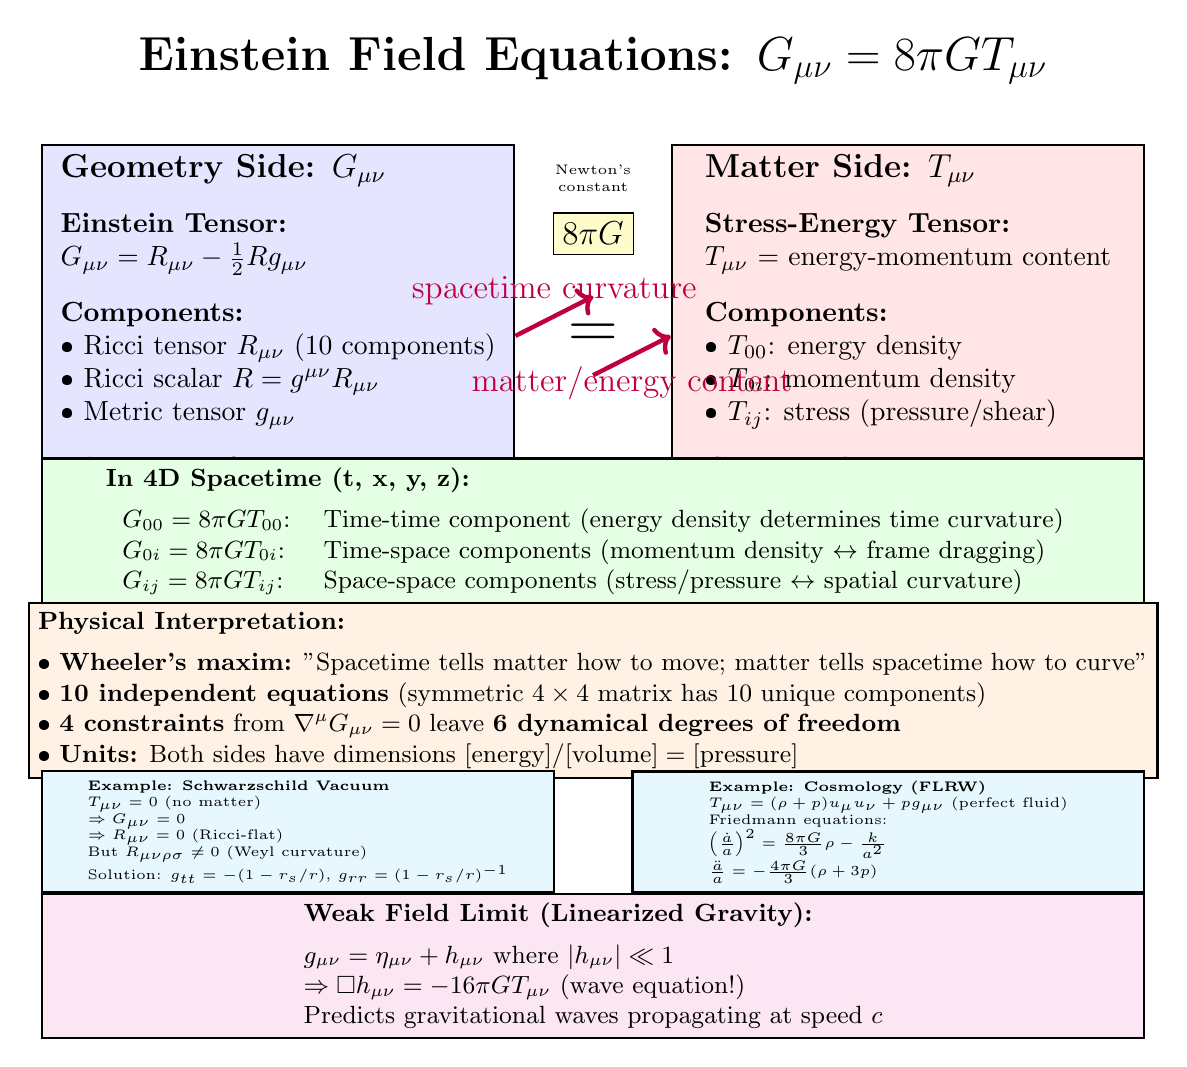
\begin{tikzpicture}[scale=1.0]

% Title
\node[font=\LARGE\bfseries] at (0,6.5) {Einstein Field Equations: $G_{\mu\nu} = 8\pi G T_{\mu\nu}$};

% Left side: Geometry (Einstein tensor)
\node[draw, thick, fill=blue!10, minimum width=6cm, minimum height=4cm, align=left] (geom) at (-4,3) {
    \textbf{\large Geometry Side: $G_{\mu\nu}$}\\[8pt]
    \textbf{Einstein Tensor:}\\
    $G_{\mu\nu} = R_{\mu\nu} - \frac{1}{2}Rg_{\mu\nu}$\\[8pt]
    \textbf{Components:}\\
    • Ricci tensor $R_{\mu\nu}$ (10 components)\\
    • Ricci scalar $R = g^{\mu\nu}R_{\mu\nu}$\\
    • Metric tensor $g_{\mu\nu}$\\[8pt]
    \textbf{Divergence-free:}\\
    $\nabla^\mu G_{\mu\nu} = 0$ (Bianchi identity)
};

% Right side: Matter (stress-energy tensor)
\node[draw, thick, fill=red!10, minimum width=6cm, minimum height=4cm, align=left] (matter) at (4,3) {
    \textbf{\large Matter Side: $T_{\mu\nu}$}\\[8pt]
    \textbf{Stress-Energy Tensor:}\\
    $T_{\mu\nu}$ = energy-momentum content\\[8pt]
    \textbf{Components:}\\
    • $T_{00}$: energy density\\
    • $T_{0i}$: momentum density\\
    • $T_{ij}$: stress (pressure/shear)\\[8pt]
    \textbf{Conserved:}\\
    $\nabla^\mu T_{\mu\nu} = 0$ (local conservation)
};

% Equals sign with constant
\node[font=\Huge] at (0,3) {$=$};
\node[draw, fill=yellow!20, font=\large] at (0,4.3) {$8\pi G$};
\node[font=\tiny, align=center] at (0,5) {Newton's\\constant};

% Arrow showing causality
\draw[->, ultra thick, purple] (geom.east) -- node[above, font=\large, text=purple] {spacetime curvature} (0,3.5);
\draw[->, ultra thick, purple] (0,2.5) -- node[below, font=\large, text=purple] {matter/energy content} (matter.west);

% Component breakdown for 4D spacetime
\node[draw, thick, fill=green!10, minimum width=14cm, align=left, font=\small] at (0,0.5) {
    \textbf{In 4D Spacetime (t, x, y, z):}\\[4pt]
    \begin{tabular}{ll}
    $G_{00} = 8\pi G T_{00}$: & Time-time component (energy density determines time curvature) \\
    $G_{0i} = 8\pi G T_{0i}$: & Time-space components (momentum density $\leftrightarrow$ frame dragging) \\
    $G_{ij} = 8\pi G T_{ij}$: & Space-space components (stress/pressure $\leftrightarrow$ spatial curvature) \\
    \end{tabular}
};

% Physical interpretation box
\node[draw, thick, fill=orange!10, minimum width=14cm, align=left, font=\small] at (0,-1.5) {
    \textbf{Physical Interpretation:}\\[4pt]
    • \textbf{Wheeler's maxim:} "Spacetime tells matter how to move; matter tells spacetime how to curve"\\
    • \textbf{10 independent equations} (symmetric $4\times4$ matrix has 10 unique components)\\
    • \textbf{4 constraints} from $\nabla^\mu G_{\mu\nu}=0$ leave \textbf{6 dynamical degrees of freedom}\\
    • \textbf{Units:} Both sides have dimensions $[\text{energy}]/[\text{volume}] = [\text{pressure}]$
};

% Example: Schwarzschild vacuum
\node[draw, thick, fill=cyan!10, minimum width=6.5cm, align=left, font=\tiny] at (-3.75,-3.3) {
    \textbf{Example: Schwarzschild Vacuum}\\
    $T_{\mu\nu} = 0$ (no matter)\\
    $\Rightarrow G_{\mu\nu} = 0$\\
    $\Rightarrow R_{\mu\nu} = 0$ (Ricci-flat)\\
    But $R_{\mu\nu\rho\sigma} \neq 0$ (Weyl curvature)\\
    Solution: $g_{tt} = -(1-r_s/r)$, $g_{rr} = (1-r_s/r)^{-1}$
};

% Example: Cosmology
\node[draw, thick, fill=cyan!10, minimum width=6.5cm, align=left, font=\tiny] at (3.75,-3.3) {
    \textbf{Example: Cosmology (FLRW)}\\
    $T_{\mu\nu} = (\rho + p)u_\mu u_\nu + p g_{\mu\nu}$ (perfect fluid)\\
    Friedmann equations:\\
    $\left(\frac{\dot{a}}{a}\right)^2 = \frac{8\pi G}{3}\rho - \frac{k}{a^2}$\\
    $\frac{\ddot{a}}{a} = -\frac{4\pi G}{3}(\rho + 3p)$
};

% Linearized limit box
\node[draw, thick, fill=magenta!10, minimum width=14cm, align=left, font=\small] at (0,-5) {
    \textbf{Weak Field Limit (Linearized Gravity):}\\[4pt]
    $g_{\mu\nu} = \eta_{\mu\nu} + h_{\mu\nu}$ where $|h_{\mu\nu}| \ll 1$\\
    $\Rightarrow \Box h_{\mu\nu} = -16\pi G T_{\mu\nu}$ (wave equation!)\\
    Predicts gravitational waves propagating at speed $c$
};

\end{tikzpicture}

\caption{Einstein field equations structure: Geometry (left, $G_{\mu\nu}$) equals matter-energy (right, $T_{\mu\nu}$). Examples: Schwarzschild (spherical star), FLRW (expanding universe), gravitational waves (ripples in spacetime). \mphys{``Matter tells spacetime how to curve; spacetime tells matter how to move'' (Wheeler).}}
\label{fig:prelim:einstein-eqns}
\end{figure}

\mex{Schwarzschild solution: $T_{\mu\nu} = 0$ (vacuum) gives black hole metric. FLRW solution: $T_{\mu\nu} = (\rho + p) u_\mu u_\nu + p g_{\mu\nu}$ (perfect fluid) gives cosmology.}

\subsection{Worked Example: Ricci Curvature of a 2-Sphere}

For a 2-sphere of radius $R$ with metric:
\begin{equation}
  ds^2 = R^2 (d\theta^2 + \sin^2\theta \, d\phi^2)
  \label{eq:prelim:sphere-metric}
\end{equation}

Computing the Christoffel symbols:
\begin{align}
  \Gamma^\theta_{\phi\phi} &= -\sin\theta \cos\theta \\
  \Gamma^\phi_{\theta\phi} = \Gamma^\phi_{\phi\theta} &= \cot\theta
\end{align}

The Riemann tensor has only one independent component (in 2D):
\begin{equation}
  R^\theta{}_{\phi\theta\phi} = \sin^2\theta
  \label{eq:prelim:sphere-riemann}
\end{equation}

Ricci tensor:
\begin{equation}
  R_{\theta\theta} = 1, \quad R_{\phi\phi} = \sin^2\theta
  \label{eq:prelim:sphere-ricci}
\end{equation}

Ricci scalar:
\begin{equation}
  R = g^{\theta\theta} R_{\theta\theta} + g^{\phi\phi} R_{\phi\phi} = \frac{1}{R^2} + \frac{1}{R^2} = \frac{2}{R^2}
  \label{eq:prelim:sphere-scalar}
\end{equation}

\textbf{Interpretation}: Positive constant curvature $R = 2/R^2$. Smaller spheres (smaller $R$) have larger curvature, as expected. The factor of 2 reflects two spatial dimensions curving.

\subsection{Bridge to Wave Operators}

To describe field dynamics in curved spacetime, we need differential operators that respect the geometry. The natural generalization of the flat-space wave operator $\Box = -\partial_t^2 + \nabla^2$ is the d'Alembertian constructed from covariant derivatives.

%-----------------------------------------------------------------------------
\section{Differential Operators in Curved Spacetime}
\label{sec:prelim:operators}
%-----------------------------------------------------------------------------

\subsection{Covariant Divergence}

The divergence of a vector field $V^\mu$ in curved space requires both the derivative of $V^\mu$ and corrections for the changing volume element:
\begin{equation}
  \nabla_\mu V^\mu = \frac{1}{\sqrt{-g}} \partial_\mu\left(\sqrt{-g}\, V^\mu\right)
  \label{eq:prelim:covariant-divergence}
\end{equation}

where $g = \det(g_{\mu\nu})$ is the determinant of the metric.

\textbf{Why $\sqrt{-g}$?} This is the volume element in curved coordinates. In flat Minkowski space with Cartesian coordinates, $g = -1$ and $\sqrt{-g} = 1$. In general coordinates, $\sqrt{-g}$ accounts for coordinate stretching and squashing.

\subsection{D'Alembertian Wave Operator}

The curved-space generalization of the wave operator acting on a scalar field $\phi$ is:
\begin{equation}
  \Box \phi = \nabla_\mu \nabla^\mu \phi = \frac{1}{\sqrt{-g}} \partial_\mu\left(\sqrt{-g}\, g^{\mu\nu} \partial_\nu \phi\right)
  \label{eq:prelim:dalembertian}
\end{equation}\index{d'Alembertian}\index{wave operator|see{d'Alembertian}}

\textbf{Physical meaning}: This operator encodes wave propagation respecting the spacetime geometry. Waves follow geodesics, not straight lines.

In Minkowski spacetime with Cartesian coordinates ($g_{\mu\nu} = \eta_{\mu\nu} = \text{diag}(-1,+1,+1,+1)$), this reduces to:
\begin{equation}
  \Box \phi = -\frac{\partial^2 \phi}{\partial t^2} + \nabla^2 \phi
  \label{eq:prelim:dalembertian-flat}
\end{equation}

where $\nabla^2 = \partial_i \partial^i$ is the flat-space Laplacian.

\textbf{Application to scalar fields}: The Aether framework uses this operator extensively in scalar field equations. The Genesis framework extends it to fractal harmonic modes. Both depend critically on getting the curved-space version right.

%-----------------------------------------------------------------------------
\section{Natural Units and the Planck Scale}
\label{sec:prelim:planck}
%-----------------------------------------------------------------------------

\subsection{Why Natural Units?}

In theoretical physics, carrying factors of $c$, $\hbar$, and $G$ through equations obscures the underlying structure. By setting $c = \hbar = 1$, we eliminate dimensional clutter and reveal physical relationships.

The speed of light $c = \SI{2.998e8}{\meter\per\second}$ sets the conversion between space and time:
\begin{equation}
  1~\text{second} = c \times 1~\text{second} = \SI{2.998e8}{\meter}
  \label{eq:prelim:c-conversion}
\end{equation}

The reduced Planck constant $\hbar = \SI{1.055e-34}{\joule\second}$ sets the conversion between energy and frequency:
\begin{equation}
  E = \hbar \omega \quad \Rightarrow \quad 1~\text{Joule} = \frac{1}{\hbar}~\text{Hz} \approx \SI{9.48e33}{\per\second}
  \label{eq:prelim:hbar-conversion}
\end{equation}

With $c = \hbar = 1$, all quantities can be expressed in powers of energy (or equivalently, inverse length):
\begin{equation}
  [E] = [m] = [T^{-1}] = [L^{-1}]
  \label{eq:prelim:natural-dimensions}
\end{equation}

\textbf{Practical use}: Write equations in natural units. To restore SI units for experimental predictions, reintroduce $c$ and $\hbar$ via dimensional analysis.

\subsection{The Planck Scale: Where Quantum Gravity Dominates}

The Planck length, mass, time, and energy\index{Planck scale}\index{Planck length}\index{Planck mass} are constructed from $G$, $\hbar$, and $c$:

%==============================================================================
% Equation: Planck scale quantities
% Source: Fundamental constants (CODATA 2018, PDG 2022)
% Provenance: Natural units and quantum gravity scale
%==============================================================================
\begin{align}
  \ell_P &= \sqrt{\frac{\hbar G}{c^3}} \approx \SI{1.616e-35}{\meter},
  \label{eq:prelim:planck-length} \\
  m_P &= \sqrt{\frac{\hbar c}{G}} \approx \SI{2.176e-8}{\kilogram} \approx \SI{1.221e19}{\giga\electronvolt/c^2},
  \label{eq:prelim:planck-mass} \\
  t_P &= \sqrt{\frac{\hbar G}{c^5}} \approx \SI{5.391e-44}{\second},
  \label{eq:prelim:planck-time} \\
  E_P &= m_P c^2 = \sqrt{\frac{\hbar c^5}{G}} \approx \SI{1.956e9}{\joule} \approx \SI{1.221e19}{\giga\electronvolt}
  \label{eq:prelim:planck-energy}
  \eqtag{M}{MATH}{T}
\end{align}
% Notes:
%   * Planck length: quantum gravity becomes dominant at $\ell_P$
%   * Planck mass: surprisingly large (~$10^{-8}$ kg, mass of a dust grain)
%   * Planck time: shortest physically meaningful time scale
%   * Planck energy: highest energy scale in quantum gravity
%   * In natural units ($c = \hbar = G = 1$): $\ell_P = m_P = t_P = E_P = 1$
%   * Relevant for Aether crystalline lattice spacing and Genesis kernel damping scales
%==============================================================================


\textbf{Numerical values}:
\begin{align}
  \ell_P &= \SI{1.616e-35}{\meter} \quad \text{(size of quantum foam fluctuations)} \\
  m_P &= \SI{2.176e-8}{\kilo\gram} = \SI{1.22e19}{\giga\electronvolt\per c^2} \quad \text{(mass where gravity becomes quantum)} \\
  t_P &= \SI{5.391e-44}{\second} \quad \text{(earliest moment describable by physics)} \\
  E_P &= \SI{1.956e9}{\joule} = \SI{1.22e19}{\giga\electronvolt} \quad \text{(energy of early-universe collisions)}
\end{align}

\textbf{Why these scales matter}:
\begin{itemize}
  \item At lengths $\ell < \ell_P$, quantum fluctuations of spacetime itself become significant. General relativity breaks down.

  \item At energies $E \sim E_P$, particles create black holes via gravitational collapse. The Schwarzschild radius $r_s = 2GM/c^2$ equals the Compton wavelength $\lambda_C = \hbar/(mc)$.

  \item The \textbf{Aether crystalline spacetime} explicitly models Planck-scale structure as a discrete lattice.

  \item The \textbf{Genesis framework} treats the Planck scale as the fundamental discretization where nodespace emerges.

  \item All unified frameworks must explain physics at the Planck scale---this is where quantum mechanics and gravity meet.
\end{itemize}

\subsection{Unit Conversions for Experimental Predictions}

When making experimental predictions, convert from natural units to SI:

\begin{table}[h]
\centering
\begin{tabular}{lcc}
\toprule
Quantity & Natural Units & SI Units \\
\midrule
Energy & $E$ & $E \times \hbar c / \ell$ \\
Mass & $m$ & $m \times \hbar / (c \ell)$ \\
Length & $\ell$ & $\ell$ \\
Time & $t$ & $t \times \ell / c$ \\
Temperature & $T$ & $T \times k_B$ \\
Cross section & $\sigma$ & $\sigma \times \ell^2$ \\
\bottomrule
\end{tabular}
\caption{Conversion factors between natural units ($c = \hbar = 1$) and SI units. Here $\ell$ is a length scale characteristic of the problem (e.g., Compton wavelength).}
\label{tab:prelim:ch01:unit-conversions}
\end{table}

\textbf{Example}: The Casimir force per unit area between parallel plates separated by $a$ is:
\begin{equation}
  F/A = -\frac{\pi^2 \hbar c}{240 a^4} \quad \text{(SI units)}
  \label{eq:prelim:casimir-si}
\end{equation}

In natural units ($\hbar = c = 1$):
\begin{equation}
  F/A = -\frac{\pi^2}{240 a^4} \quad \text{(natural units)}
  \label{eq:prelim:casimir-natural}
\end{equation}

The natural-units version reveals the essential scaling: force goes as $a^{-4}$. The SI version gives the numerical value for experiment.

\subsection{Bridge to Quantum Formalism}

We have established the geometry of spacetime. But quantum mechanics requires a different mathematical language: Hilbert spaces, operators, and probability amplitudes. Unifying gravity with quantum mechanics demands fluency in both languages.

%-----------------------------------------------------------------------------
\section{Quantum Mechanics: Hilbert Spaces and Operators}
\label{sec:prelim:quantum}
%-----------------------------------------------------------------------------

\subsection{Why Hilbert Spaces?}

Classical physics uses phase space: a point represents a system's state. Quantum mechanics uses \textbf{state vectors} in a complex Hilbert space $\mathcal{H}$. Why?

Experiments revealed:
\begin{itemize}
  \item \textbf{Superposition}: A quantum system can be in multiple classical states simultaneously (e.g., electron in both spin-up and spin-down).
  \item \textbf{Interference}: Probabilities do not add; probability amplitudes (complex numbers) add, then square to get probabilities.
  \item \textbf{Entanglement}: Composite systems cannot always be factored into independent subsystems.
\end{itemize}

Complex vector spaces naturally encode these features. The mathematical structure is:

\begin{itemize}
  \item \textbf{Ket} $\ket{\psi}$: A quantum state vector in $\mathcal{H}$.
  \item \textbf{Bra} $\bra{\phi}$: The dual vector, representing a linear functional $\mathcal{H} \to \mathbb{C}$.
  \item \textbf{Inner product} $\braket{\phi|\psi}$: A complex number satisfying:
  \begin{align}
    \braket{\phi|\psi} &= \braket{\psi|\phi}^* \quad \text{(conjugate symmetry)} \\
    \braket{\psi|\psi} &\geq 0 \quad \text{(positive definite)} \\
    \braket{\psi|\psi} &= 0 \Leftrightarrow \ket{\psi} = 0 \quad \text{(definiteness)}
  \end{align}
\end{itemize}

\textbf{Normalization}: Physical states are normalized: $\braket{\psi|\psi} = 1$. This ensures probabilities sum to 1.

\mxref{Quantum formalism connects to differential geometry via geometric phase (Berry phase) and fiber bundles. See \S\ref{sec:geometric-phase} for gauge field interpretation of quantum phases.}

%-----------------------------------------------------------------------------
% QUANTUM FORMALISM: Complete Hierarchy
%-----------------------------------------------------------------------------

\begin{figure}[htbp]
\centering
% Quantum Mechanics Mathematical Structure
% Comprehensive visual guide to the formalism used in quantum field theory

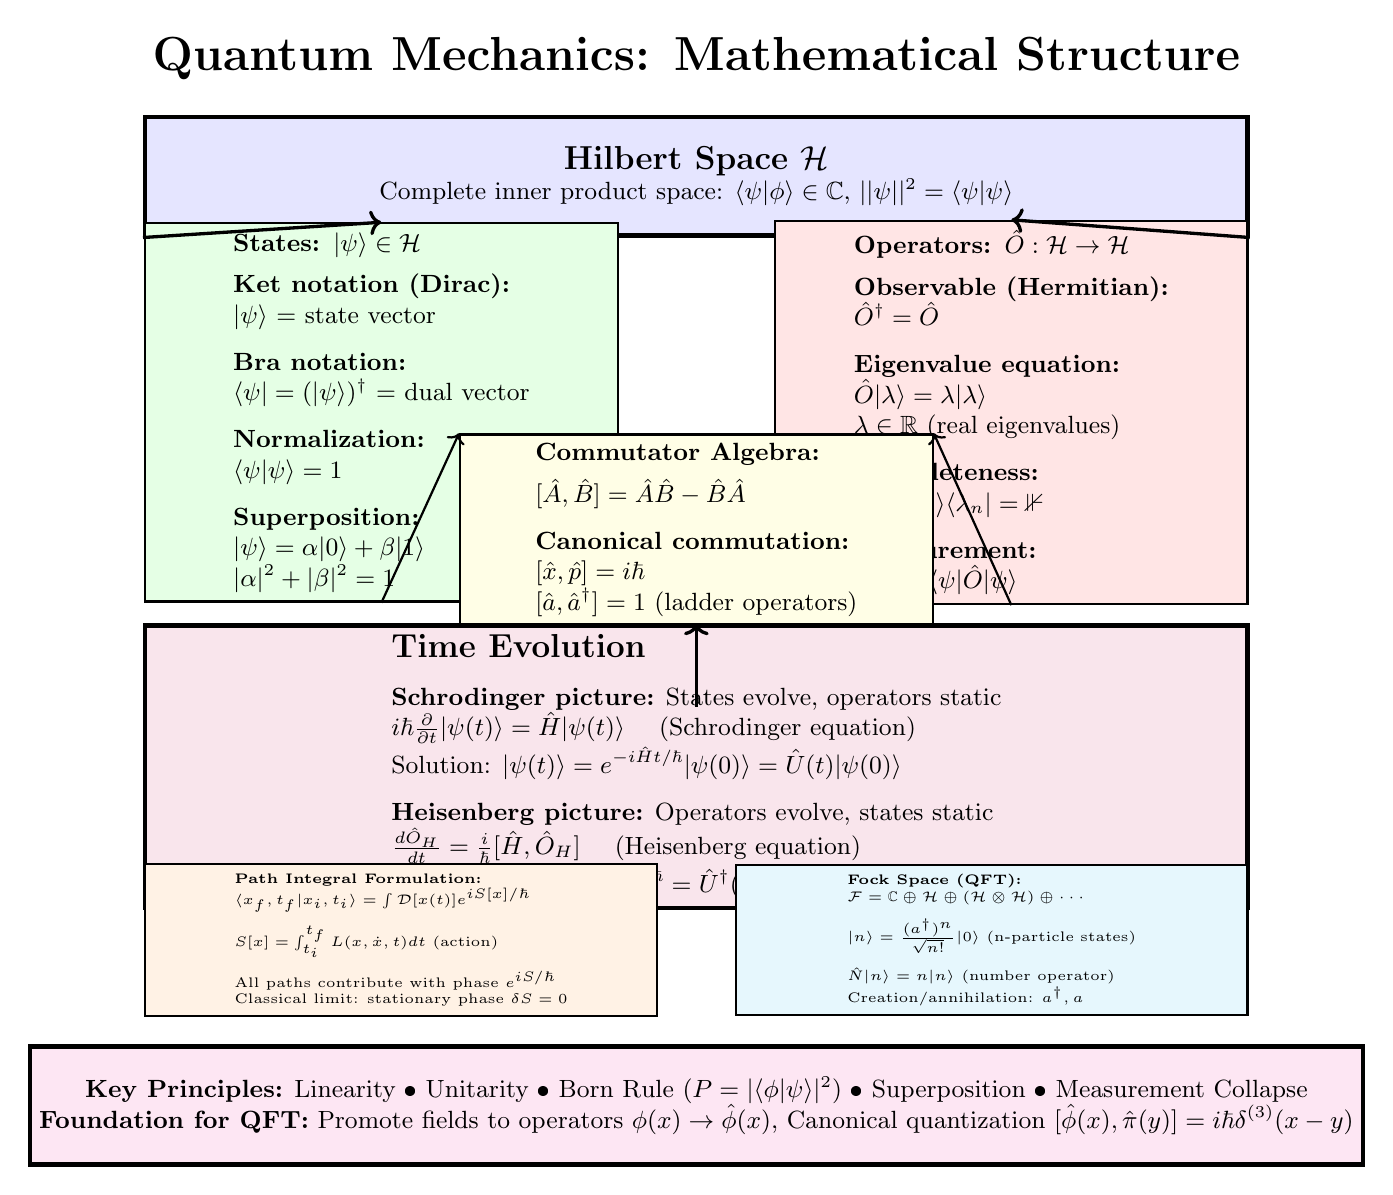
\begin{tikzpicture}[scale=1.0, every node/.style={font=\small}]

% Title
\node[font=\LARGE\bfseries] at (0,8) {Quantum Mechanics: Mathematical Structure};

% Hilbert Space (top level)
\node[draw, ultra thick, fill=blue!10, minimum width=14cm, minimum height=1.5cm, align=center] (hilbert) at (0,6.5) {
    \textbf{\large Hilbert Space $\mathcal{H}$}\\
    Complete inner product space: $\langle\psi|\phi\rangle \in \mathbb{C}$, $||\psi||^2 = \langle\psi|\psi\rangle$
};

% States (left branch)
\node[draw, thick, fill=green!10, minimum width=6cm, minimum height=3cm, align=left] (states) at (-4,3.5) {
    \textbf{States: $|\psi\rangle \in \mathcal{H}$}\\[4pt]
    \textbf{Ket notation (Dirac):}\\
    $|\psi\rangle$ = state vector\\[6pt]
    \textbf{Bra notation:}\\
    $\langle\psi| = (|\psi\rangle)^\dagger$ = dual vector\\[6pt]
    \textbf{Normalization:}\\
    $\langle\psi|\psi\rangle = 1$\\[6pt]
    \textbf{Superposition:}\\
    $|\psi\rangle = \alpha|0\rangle + \beta|1\rangle$\\
    $|\alpha|^2 + |\beta|^2 = 1$
};

% Operators (right branch)
\node[draw, thick, fill=red!10, minimum width=6cm, minimum height=3cm, align=left] (ops) at (4,3.5) {
    \textbf{Operators: $\hat{O}: \mathcal{H} \to \mathcal{H}$}\\[4pt]
    \textbf{Observable (Hermitian):}\\
    $\hat{O}^\dagger = \hat{O}$\\[6pt]
    \textbf{Eigenvalue equation:}\\
    $\hat{O}|\lambda\rangle = \lambda|\lambda\rangle$\\
    $\lambda \in \mathbb{R}$ (real eigenvalues)\\[6pt]
    \textbf{Completeness:}\\
    $\sum_n |\lambda_n\rangle\langle\lambda_n| = \mathbb{1}$\\[6pt]
    \textbf{Measurement:}\\
    $\langle\hat{O}\rangle = \langle\psi|\hat{O}|\psi\rangle$
};

% Arrows connecting
\draw[->, very thick] (hilbert.south west) -- (states.north);
\draw[->, very thick] (hilbert.south east) -- (ops.north);

% Commutator algebra (middle)
\node[draw, thick, fill=yellow!10, minimum width=6cm, minimum height=2cm, align=left] (comm) at (0,1.5) {
    \textbf{Commutator Algebra:}\\[4pt]
    $[\hat{A}, \hat{B}] = \hat{A}\hat{B} - \hat{B}\hat{A}$\\[6pt]
    \textbf{Canonical commutation:}\\
    $[\hat{x}, \hat{p}] = i\hbar$\\
    $[\hat{a}, \hat{a}^\dagger] = 1$ (ladder operators)\\[6pt]
    \textbf{Uncertainty principle:}\\
    $\Delta A \cdot \Delta B \geq \frac{1}{2}|\langle[\hat{A},\hat{B}]\rangle|$
};

% Arrows from states and operators to commutator
\draw[->, thick] (states.south) -- (comm.north west);
\draw[->, thick] (ops.south) -- (comm.north east);

% Time evolution (bottom level)
\node[draw, ultra thick, fill=purple!10, minimum width=14cm, minimum height=2.5cm, align=left] (time) at (0,-1) {
    \textbf{\large Time Evolution}\\[6pt]
    \textbf{Schrodinger picture:} States evolve, operators static\\
    $i\hbar\frac{\partial}{\partial t}|\psi(t)\rangle = \hat{H}|\psi(t)\rangle$ \quad (Schrodinger equation)\\
    Solution: $|\psi(t)\rangle = e^{-i\hat{H}t/\hbar}|\psi(0)\rangle = \hat{U}(t)|\psi(0)\rangle$\\[6pt]
    \textbf{Heisenberg picture:} Operators evolve, states static\\
    $\frac{d\hat{O}_H}{dt} = \frac{i}{\hbar}[\hat{H}, \hat{O}_H]$ \quad (Heisenberg equation)\\
    $\hat{O}_H(t) = e^{i\hat{H}t/\hbar}\hat{O}e^{-i\hat{H}t/\hbar} = \hat{U}^\dagger(t)\hat{O}\hat{U}(t)$
};

% Arrow from commutator to time evolution
\draw[->, very thick] (comm.south) -- (time.north);

% Path integral (bottom box)
\node[draw, thick, fill=orange!10, minimum width=6.5cm, minimum height=1.8cm, align=left, font=\tiny] (path) at (-3.75,-3.2) {
    \textbf{Path Integral Formulation:}\\
    $\langle x_f, t_f | x_i, t_i \rangle = \int \mathcal{D}[x(t)] e^{iS[x]/\hbar}$\\[4pt]
    $S[x] = \int_{t_i}^{t_f} L(x, \dot{x}, t) dt$ (action)\\[4pt]
    All paths contribute with phase $e^{iS/\hbar}$\\
    Classical limit: stationary phase $\delta S = 0$
};

% Fock space (bottom right box)
\node[draw, thick, fill=cyan!10, minimum width=6.5cm, minimum height=1.8cm, align=left, font=\tiny] (fock) at (3.75,-3.2) {
    \textbf{Fock Space (QFT):}\\
    $\mathcal{F} = \mathbb{C} \oplus \mathcal{H} \oplus (\mathcal{H} \otimes \mathcal{H}) \oplus \cdots$\\[4pt]
    $|n\rangle = \frac{(a^\dagger)^n}{\sqrt{n!}}|0\rangle$ (n-particle states)\\[4pt]
    $\hat{N}|n\rangle = n|n\rangle$ (number operator)\\
    Creation/annihilation: $a^\dagger, a$
};

% Key principles box
\node[draw, ultra thick, fill=magenta!10, minimum width=14cm, minimum height=1.5cm, align=center] (key) at (0,-5.3) {
    \textbf{Key Principles:} Linearity • Unitarity • Born Rule ($P = |\langle\phi|\psi\rangle|^2$) • Superposition • Measurement Collapse\\
    \textbf{Foundation for QFT:} Promote fields to operators $\phi(x) \to \hat{\phi}(x)$, Canonical quantization $[\hat{\phi}(x), \hat{\pi}(y)] = i\hbar\delta^{(3)}(x-y)$
};

\end{tikzpicture}

\caption{Quantum mechanics formalism hierarchy: Hilbert space $\mathcal{H}$ (infinite-dimensional vector space) → States $\ket{\psi}$ → Operators $\hat{A}$ (observables) → Dynamics (Schr\"odinger equation $i\hbar \partial_t \ket{\psi} = \hat{H} \ket{\psi}$) → Measurement (Born rule $P = |\braket{\phi|\psi}|^2$). \mphys{Complete structure encodes superposition, interference, entanglement.}}
\label{fig:prelim:quantum-structure}
\end{figure}

\mdim{Quantum mechanics dimensionality: $[\hbar] = [\text{energy}] \cdot [\text{time}] = [\text{action}]$. Schr\"odinger equation: $[\partial_t \ket{\psi}] = [\text{time}]^{-1} \times [\text{state}]$, $[\hat{H}\ket{\psi}] = [\text{energy}] \times [\text{state}] = \hbar \times [\text{time}]^{-1} \times [\text{state}]$. Dimensional consistency requires $\hbar$.}

\subsection{Operators Represent Observables}

In quantum mechanics, every measurable quantity (energy, momentum, position, spin) is represented by a \textbf{Hermitian operator}\index{Hermitian operator}\index{operator!Hermitian}\index{observable|see{Hermitian operator}} $\hat{A}$ satisfying $\hat{A}^\dagger = \hat{A}$.

\textbf{Expectation value} of $\hat{A}$ in state $\ket{\psi}$:
\begin{equation}
  \langle \hat{A} \rangle = \bra{\psi} \hat{A} \ket{\psi}
  \label{eq:prelim:expectation-value}
\end{equation}

\textbf{Eigenvalue equation}:
\begin{equation}
  \hat{A} \ket{a} = a \ket{a}
  \label{eq:prelim:eigenvalue}
\end{equation}

where $a$ is a real eigenvalue (possible measurement outcome) and $\ket{a}$ is the corresponding eigenstate.

\textbf{Measurement postulate}: Measuring $\hat{A}$ yields one of its eigenvalues $a$ with probability:
\begin{equation}
  P(a) = |\braket{a|\psi}|^2
  \label{eq:prelim:born-rule}
\end{equation}

After measurement, the state collapses to $\ket{a}$ (or the eigenspace corresponding to $a$ if degenerate).

\subsection{Canonical Commutation Relations}

The fundamental quantum rule is that position $\hat{x}^i$ and momentum $\hat{p}_j$ do not commute\index{commutation relations}\index{canonical commutation relations}:

%==============================================================================
% Equation: Canonical commutation relations (position-momentum)
% Source: Quantum mechanics foundations (Dirac, Sakurai, Griffiths)
% Provenance: Quantum operator formalism preliminaries
%==============================================================================
\begin{align}
  [\hat{x}^i, \hat{p}_j] &= \imag \hbar \delta^i_j,
  \label{eq:prelim:commutator-xp}
  \label{eq:commutator:canonical} \\
  [\hat{x}^i, \hat{x}^j] &= 0,
  \label{eq:prelim:commutator-xx} \\
  [\hat{p}_i, \hat{p}_j] &= 0
  \label{eq:prelim:commutator-pp}
  \eqtag{M}{QM}{T}
\end{align}
% Notes:
%   * Fundamental commutation relations of quantum mechanics
%   * $\delta^i_j$ is Kronecker delta ($i,j = 1,2,3$ spatial indices)
%   * In natural units ($\hbar = 1$): $[\hat{x}^i, \hat{p}_j] = \imag \delta^i_j$
%   * Implies Heisenberg uncertainty principle: $\Delta x \Delta p \geq \hbar/2$
%   * Position representation: $\hat{p}_i = -\imag \hbar \partial/\partial x^i$
%   * Momentum representation: $\hat{x}^i = \imag \hbar \partial/\partial p_i$
%   * Generalized to field theory (see Ch. 8 scalar field quantization)
%==============================================================================


\textbf{Physical meaning}: You cannot simultaneously measure position and momentum with arbitrary precision. This is the \textbf{Heisenberg uncertainty principle}\index{Heisenberg uncertainty principle}\index{uncertainty principle}:
\begin{equation}
  \Delta x \, \Delta p \geq \frac{\hbar}{2}
  \label{eq:prelim:heisenberg}
\end{equation}

The commutator $[\hat{A}, \hat{B}] \equiv \hat{A}\hat{B} - \hat{B}\hat{A}$ quantifies incompatibility:
\begin{itemize}
  \item If $[\hat{A}, \hat{B}] = 0$: Operators commute, can be simultaneously measured.
  \item If $[\hat{A}, \hat{B}] \neq 0$: Operators do not commute, measurement of one disturbs the other.
\end{itemize}

\textbf{Application to unified frameworks}: Scalar fields in the Aether framework are promoted to quantum operators satisfying commutation relations analogous to equation~\eqref{eq:commutator:canonical}. The Genesis framework extends this to fractal mode operators.

\subsection{Time Evolution: The Schrodinger Equation}

How do quantum states change with time? The \textbf{Schr\"odinger equation}\index{Schr\"odinger equation}\index{time evolution!quantum} governs time evolution:

%==============================================================================
% Equation: Time-dependent Schrodinger equation
% Source: Quantum mechanics foundations (Dirac 1930, Sakurai Ch. 2)
% Provenance: Quantum operator formalism preliminaries
%==============================================================================
\begin{equation}
  \imag \hbar \frac{\partial}{\partial t} \ket{\psi(t)} = \hat{H} \ket{\psi(t)}
  \eqtag{M}{QM}{T}
  \label{eq:prelim:schrodinger-equation}
\end{equation}
% Notes:
%   * Governs time evolution of quantum states
%   * $\hat{H}$ is the Hamiltonian operator (total energy)
%   * In natural units ($\hbar = 1$): $\imag \partial_t \ket{\psi} = \hat{H} \ket{\psi}$
%   * Position representation: $\imag \hbar \partial_t \psi(\mathbf{x},t) = \hat{H} \psi(\mathbf{x},t)$
%   * For non-relativistic particle: $\hat{H} = -\frac{\hbar^2}{2m} \nabla^2 + V(\mathbf{x})$
%   * Time-independent case: $\hat{H} \ket{E} = E \ket{E}$ (eigenvalue problem)
%   * Unitarity: $\frac{\dd}{\dd t} \braket{\psi|\psi} = 0$ (probability conservation)
%   * Extended in Aether/Genesis frameworks with additional field couplings
%==============================================================================


where $\hat{H}$ is the \textbf{Hamiltonian operator}\index{Hamiltonian}\index{operator!Hamiltonian} representing total energy.

For a non-relativistic particle in potential $V(\mathbf{x})$:
\begin{equation}
  \hat{H} = \frac{\hat{p}^2}{2m} + V(\hat{x}) = -\frac{\hbar^2}{2m} \nabla^2 + V(\mathbf{x})
  \label{eq:prelim:hamiltonian-nonrel}
\end{equation}

\textbf{Formal solution} (for time-independent $\hat{H}$):
\begin{equation}
  \ket{\psi(t)} = \exp\left(-\frac{i}{\hbar} \hat{H} t\right) \ket{\psi(0)}
  \label{eq:prelim:time-evolution}
\end{equation}

\textbf{Energy eigenstates} (stationary states):
\begin{equation}
  \hat{H} \ket{E} = E \ket{E} \quad \Rightarrow \quad \ket{\psi(t)} = e^{-iEt/\hbar} \ket{E}
  \label{eq:prelim:energy-eigenstate}
\end{equation}

Only the phase rotates; the probability density $|\psi(\mathbf{x}, t)|^2$ is time-independent.

\textbf{Connection to field theory}: In the Aether and Genesis frameworks, the Hamiltonian includes field energy, ZPE coupling, and potentially non-local terms encoding quantum foam effects.

\subsection{Density Operators and Mixed States}

Pure quantum states $\ket{\psi}$ describe complete knowledge. When uncertainty exists (thermal fluctuations, environmental decoherence), we use \textbf{density operators}:
\begin{equation}
  \hat{\rho} = \sum_i p_i \ket{\psi_i}\bra{\psi_i}
  \label{eq:prelim:density-operator}
\end{equation}

where $p_i$ are classical probabilities with $\sum_i p_i = 1$.

\textbf{Expectation value}:
\begin{equation}
  \langle \hat{A} \rangle = \mathrm{Tr}(\hat{\rho} \hat{A})
  \label{eq:prelim:expectation-density}
\end{equation}

\textbf{Von Neumann entropy} (quantum information content):
\begin{equation}
  S = -k_B \, \mathrm{Tr}(\hat{\rho} \ln \hat{\rho})
  \label{eq:prelim:von-neumann-entropy}
\end{equation}

Pure states have $S = 0$ (zero entropy). Maximally mixed states have maximum entropy.

\textbf{Application to ZPE coherence}: The Genesis framework models ZPE states as mixed states transitioning to coherent states under specific geometric conditions. The von Neumann entropy tracks this coherence.

\subsection{Bridge to Spectral Methods}

Both curved spacetime geometry and quantum mechanics rely on spectral decomposition: expanding fields in basis functions. This motivates Fourier analysis, which is essential for field theory and fractal harmonics.

%-----------------------------------------------------------------------------
\section{Fourier Analysis and Spectral Decomposition}
\label{sec:prelim:fourier}
%-----------------------------------------------------------------------------

\subsection{Why Fourier Transforms?}

Most physical fields are superpositions of wave modes. Fourier analysis decomposes arbitrary fields into plane waves with definite frequency and wavelength. This is essential because:
\begin{itemize}
  \item Wave equations are diagonal in frequency space (each mode evolves independently).
  \item Quantum field theory describes particles as excitations of Fourier modes.
  \item Experimental measurements often target specific frequency bands.
\end{itemize}

\subsection{Fourier Transform and Inverse}

The Fourier transform\index{Fourier transform}\index{spectral decomposition} of a function $f(t)$ is:

%==============================================================================
% Equation: Fourier transform (time to frequency domain)
% Source: Standard Fourier analysis (Arfken, Bracewell, Stein-Shakarchi)
% Provenance: Mathematical preliminaries for spectral analysis
%==============================================================================
\begin{equation}
  \tilde{f}(\omega) = \int_{-\infty}^\infty f(t) \, \ee^{\imag \omega t} \, \dd t
  \eqtag{M}{MATH}{T}
  \label{eq:prelim:fourier-transform-def}
\end{equation}
% Notes:
%   * $f(t)$: function in time domain
%   * $\tilde{f}(\omega)$: Fourier transform in frequency domain
%   * Convention: positive $\imag \omega t$ in forward transform
%   * Inverse transform: $f(t) = \frac{1}{2\pi} \int \tilde{f}(\omega) \ee^{-\imag \omega t} \dd\omega$
%   * Parseval's theorem: $\int |f(t)|^2 \dd t = \frac{1}{2\pi} \int |\tilde{f}(\omega)|^2 \dd\omega$
%   * 3D spatial version: $\tilde{f}(\mathbf{k}) = \int f(\mathbf{x}) \ee^{\imag \mathbf{k} \cdot \mathbf{x}} \dd^3 x$
%   * Essential for Genesis fractal harmonic analysis and Aether spectral decomposition
%==============================================================================


The inverse Fourier transform:
\begin{equation}
  f(t) = \frac{1}{2\pi} \int_{-\infty}^\infty \tilde{f}(\omega) \, e^{-i \omega t} \, d\omega
  \label{eq:prelim:fourier-inverse}
\end{equation}

\textbf{Spatial Fourier transform}:
\begin{equation}
  \tilde{f}(\mathbf{k}) = \int f(\mathbf{x}) \, e^{i \mathbf{k} \cdot \mathbf{x}} \, d^3 x
  \label{eq:prelim:fourier-3d}
\end{equation}

\textbf{Parseval's theorem} (energy conservation):
\begin{equation}
  \int_{-\infty}^\infty |f(t)|^2 \, dt = \frac{1}{2\pi} \int_{-\infty}^\infty |\tilde{f}(\omega)|^2 \, d\omega
  \label{eq:prelim:parseval}
\end{equation}

Energy in time domain equals energy in frequency domain. This is essential for understanding power spectra in scalar field dynamics.

\subsection{Spectral Decomposition of Operators}

A Hermitian operator $\hat{A}$ can be decomposed into its eigenstates:

\textbf{Discrete spectrum}:
\begin{equation}
  \hat{A} = \sum_n a_n \ket{a_n}\bra{a_n}
  \label{eq:prelim:spectral-discrete}
\end{equation}

\textbf{Continuous spectrum}:
\begin{equation}
  \hat{A} = \int a \ket{a}\bra{a} \, da
  \label{eq:prelim:spectral-continuous}
\end{equation}

\textbf{Application to fields}: Scalar field $\hat{\phi}(\mathbf{x})$ in quantum field theory is decomposed into creation/annihilation operators for each momentum mode $\mathbf{k}$. The Aether framework uses this extensively in ZPE quantization.

\subsection{Connection to Unified Framework}

The Genesis framework employs fractal harmonic analysis---a generalization of Fourier transforms to self-similar geometries. Understanding standard Fourier methods is the essential foundation.

%-----------------------------------------------------------------------------
\section{Summary and Forward Look}
\label{sec:prelim:summary}
%-----------------------------------------------------------------------------

We have established the core mathematical language required for unified field theory:

\begin{enumerate}
  \item \textbf{Differential geometry}: Metric tensor, Christoffel symbols, covariant derivatives, Riemann curvature, Einstein tensor---the language of curved spacetime and gravity.

  \item \textbf{Natural units}: Planck scale quantities that reveal where quantum gravity dominates. All unified frameworks must address Planck-scale physics.

  \item \textbf{Quantum formalism}: Hilbert spaces, operators, commutation relations, Schrodinger equation, density operators---the language of quantum mechanics.

  \item \textbf{Spectral methods}: Fourier analysis for decomposing fields into modes, essential for field quantization and harmonic analysis.
\end{enumerate}

%=============================================================================
% ADVANCED INTEGRATION: Cross-Cutting Topics & Comprehensive Analysis
%=============================================================================

\subsection{Advanced Integration: Geodesics, Dimensional Analysis, and Comprehensive Comparisons}

The following sections synthesize the mathematical tools we've developed, providing cross-cutting perspectives and comprehensive reference material.

%-----------------------------------------------------------------------------
% Geodesic Equation: Complete Treatment
%-----------------------------------------------------------------------------

\subsubsection{Geodesic Equation and Free-Fall Trajectories}

\begin{figure}[htbp]
\centering
% Geodesic Equation Visualization
% Demonstrates free fall in curved spacetime as straightest possible path
% Physical interpretation: extremal proper time, freely falling reference frame

\begin{figure}[htbp]
\centering
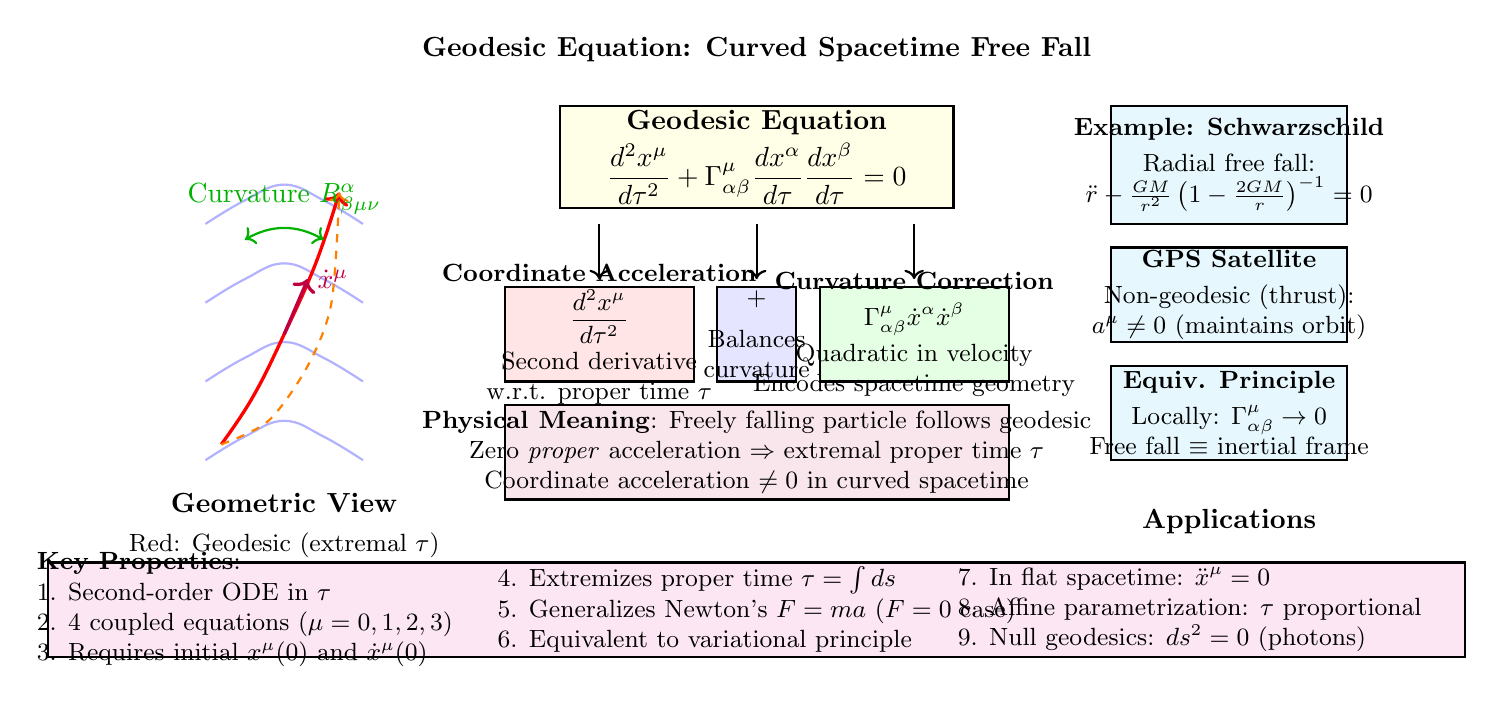
\begin{tikzpicture}[scale=1.0]
    % Title
    \node[anchor=north] at (0,5.5) {\textbf{Geodesic Equation: Curved Spacetime Free Fall}};
    
    % Left side: Curved surface representation
    \begin{scope}[xshift=-6cm]
        % Curved surface grid
        \draw[blue!30, thick] plot[smooth, tension=0.7] coordinates {(-1,0) (-0.5,0.3) (0,0.5) (0.5,0.3) (1,0)};
        \draw[blue!30, thick] plot[smooth, tension=0.7] coordinates {(-1,1) (-0.5,1.3) (0,1.5) (0.5,1.3) (1,1)};
        \draw[blue!30, thick] plot[smooth, tension=0.7] coordinates {(-1,2) (-0.5,2.3) (0,2.5) (0.5,2.3) (1,2)};
        \draw[blue!30, thick] plot[smooth, tension=0.7] coordinates {(-1,3) (-0.5,3.3) (0,3.5) (0.5,3.3) (1,3)};
        
        % Geodesic path (red, thick)
        \draw[red, very thick, ->] plot[smooth, tension=0.7] coordinates {
            (-0.8,0.2) (-0.4,0.8) (0,1.6) (0.4,2.5) (0.7,3.4)
        };
        
        % Alternative non-geodesic path (dashed, orange)
        \draw[orange, thick, dashed, ->] plot[smooth, tension=0.5] coordinates {
            (-0.8,0.2) (-0.2,0.5) (0.3,1.2) (0.6,2.0) (0.7,3.4)
        };
        
        % Tangent vector
        \draw[->, purple, very thick] (0,1.6) -- (0.3,2.3);
        \node[purple, right] at (0.3,2.3) {$\dot{x}^\mu$};
        
        % Curvature annotation
        \draw[<->, green!70!black, thick] (-0.5,2.8) to[bend left=30] (0.5,2.8);
        \node[green!70!black, above] at (0,3.0) {Curvature $R^\alpha_{\beta\mu\nu}$};
        
        \node[below] at (0,-0.3) {\textbf{Geometric View}};
        \node[below, align=center, font=\small] at (0,-0.8) {
            Red: Geodesic (extremal $\tau$)\\
            Orange: Non-geodesic (accelerated)
        };
    \end{scope}
    
    % Center: Equation breakdown
    \begin{scope}
        % Main equation box
        \draw[thick, fill=yellow!10] (-2.5,4.5) rectangle (2.5,3.2);
        \node[align=center] at (0,3.85) {
            \textbf{Geodesic Equation}\\[2pt]
            $\displaystyle \frac{d^2 x^\mu}{d\tau^2} + \Gamma^\mu_{\alpha\beta} \frac{dx^\alpha}{d\tau}\frac{dx^\beta}{d\tau} = 0$
        };
        
        % Component breakdown
        \draw[->, thick] (-2,3.0) -- (-2,2.3);
        \draw[->, thick] (0,3.0) -- (0,2.3);
        \draw[->, thick] (2,3.0) -- (2,2.3);
        
        % Acceleration term
        \draw[thick, fill=red!10] (-3.2,2.2) rectangle (-0.8,1.0);
        \node[align=center, font=\small] at (-2,1.6) {
            \textbf{Coordinate Acceleration}\\[2pt]
            $\displaystyle \frac{d^2 x^\mu}{d\tau^2}$\\[2pt]
            Second derivative\\
            w.r.t. proper time $\tau$
        };
        
        % Connection term
        \draw[thick, fill=blue!10] (-0.5,2.2) rectangle (0.5,1.0);
        \node[align=center, font=\small] at (0,1.6) {
            \textbf{$+$}\\[4pt]
            Balances\\
            curvature
        };
        
        % Christoffel velocity term
        \draw[thick, fill=green!10] (0.8,2.2) rectangle (3.2,1.0);
        \node[align=center, font=\small] at (2,1.6) {
            \textbf{Curvature Correction}\\[2pt]
            $\Gamma^\mu_{\alpha\beta} \dot{x}^\alpha\dot{x}^\beta$\\[2pt]
            Quadratic in velocity\\
            Encodes spacetime geometry
        };
        
        % Physical interpretation
        \draw[thick, fill=purple!10] (-3.2,0.7) rectangle (3.2,-0.5);
        \node[align=center, font=\small] at (0,0.1) {
            \textbf{Physical Meaning}: Freely falling particle follows geodesic\\
            Zero \textit{proper} acceleration $\Rightarrow$ extremal proper time $\tau$\\
            Coordinate acceleration $\neq 0$ in curved spacetime
        };
    \end{scope}
    
    % Right side: Examples
    \begin{scope}[xshift=6cm]
        % Example 1: Schwarzschild
        \draw[thick, fill=cyan!10] (-1.5,4.5) rectangle (1.5,3.0);
        \node[align=center, font=\small] at (0,3.75) {
            \textbf{Example: Schwarzschild}\\[2pt]
            Radial free fall:\\
            $\ddot{r} - \frac{GM}{r^2}\left(1-\frac{2GM}{r}\right)^{-1} = 0$
        };
        
        % Example 2: GPS satellite
        \draw[thick, fill=cyan!10] (-1.5,2.7) rectangle (1.5,1.5);
        \node[align=center, font=\small] at (0,2.1) {
            \textbf{GPS Satellite}\\[2pt]
            Non-geodesic (thrust):\\
            $a^\mu \neq 0$ (maintains orbit)
        };
        
        % Example 3: Equivalence principle
        \draw[thick, fill=cyan!10] (-1.5,1.2) rectangle (1.5,0.0);
        \node[align=center, font=\small] at (0,0.6) {
            \textbf{Equiv. Principle}\\[2pt]
            Locally: $\Gamma^\mu_{\alpha\beta} \to 0$\\
            Free fall $\equiv$ inertial frame
        };
        
        \node[below, align=center] at (0,-0.5) {\textbf{Applications}};
    \end{scope}
    
    % Bottom: Key properties
    \draw[thick, fill=magenta!10] (-9,-1.3) rectangle (9,-2.5);
    \node[align=left, font=\small] at (-6.5,-1.9) {
        \textbf{Key Properties}:\\
        1. Second-order ODE in $\tau$\\
        2. 4 coupled equations ($\mu = 0,1,2,3$)\\
        3. Requires initial $x^\mu(0)$ and $\dot{x}^\mu(0)$
    };
    \node[align=left, font=\small] at (0,-1.9) {
        4. Extremizes proper time $\tau = \int ds$\\
        5. Generalizes Newton's $F = ma$ ($F=0$ case)\\
        6. Equivalent to variational principle
    };
    \node[align=left, font=\small] at (5.5,-1.9) {
        7. In flat spacetime: $\ddot{x}^\mu = 0$\\
        8. Affine parametrization: $\tau$ proportional\\
        9. Null geodesics: $ds^2 = 0$ (photons)
    };
    
\end{tikzpicture}
\caption{Geodesic equation visualization showing free fall as extremal proper time path in curved spacetime. Left: geometric interpretation with geodesic (red) vs non-geodesic (orange) paths. Center: equation component breakdown. Right: physical examples (Schwarzschild, GPS, equivalence principle). Bottom: key mathematical and physical properties.}
\label{fig:geodesic_equation}
\end{figure}

\caption{Geodesic equation structure: $d^2 x^\mu/d\tau^2 = -\Gamma^\mu_{\nu\rho} (dx^\nu/d\tau)(dx^\rho/d\tau)$. Left: coordinate acceleration. Right: curvature correction (Christoffel term). \mphys{Free particles follow geodesics---\"straight lines\" in curved spacetime.}}
\label{fig:prelim:geodesic-equation}
\end{figure}

The geodesic equation describes how particles move under gravity alone (no other forces). It is the relativistic generalization of Newton's first law:

\begin{equation}
  \frac{d^2 x^\mu}{d\tau^2} + \Gamma^\mu_{\nu\rho} \frac{dx^\nu}{d\tau} \frac{dx^\rho}{d\tau} = 0
  \label{eq:prelim:geodesic-eq-full}
\end{equation}

where $\tau$ is proper time along the worldline.

\textbf{Physical interpretation}:
\begin{itemize}
  \item \textbf{Left term}: Coordinate acceleration $d^2 x^\mu/d\tau^2$ (how fast coordinates change).
  \item \textbf{Right term}: Curvature correction $\Gamma^\mu_{\nu\rho} u^\nu u^\rho$ (how curved geometry affects motion).
\end{itemize}

\textbf{Examples}:
\begin{itemize}
  \item \textbf{Schwarzschild geodesics}: Planetary orbits, GPS satellite trajectories, light bending.
  \item \textbf{GPS application}: Radial geodesic gives time dilation $dt/d\tau = (1 - 2GM/rc^2)^{-1/2}$.
  \item \textbf{Equivalence principle}: Locally, geodesic motion is indistinguishable from inertial motion in flat space.
\end{itemize}

\textbf{Key properties}:
\begin{enumerate}
  \item Geodesics are extremal paths (shortest or longest proper time).
  \item Four-velocity $u^\mu = dx^\mu/d\tau$ is tangent vector to geodesic.
  \item Normalization: $g_{\mu\nu} u^\mu u^\nu = -c^2$ (timelike), $0$ (null), $+1$ (spacelike).
  \item Conserved quantities arise from Killing vectors (symmetries of metric).
\end{enumerate}

%-----------------------------------------------------------------------------
% Light Cone Structure in Curved Spacetime
%-----------------------------------------------------------------------------

\subsubsection{Causal Structure and Light Cones}

\begin{figure}[htbp]
\centering
% Light Cone Structure in Curved Spacetime
% Demonstrates tipping and deformation of light cones near massive objects
% Foundation for causal structure and event horizons

\begin{figure}[htbp]
\centering
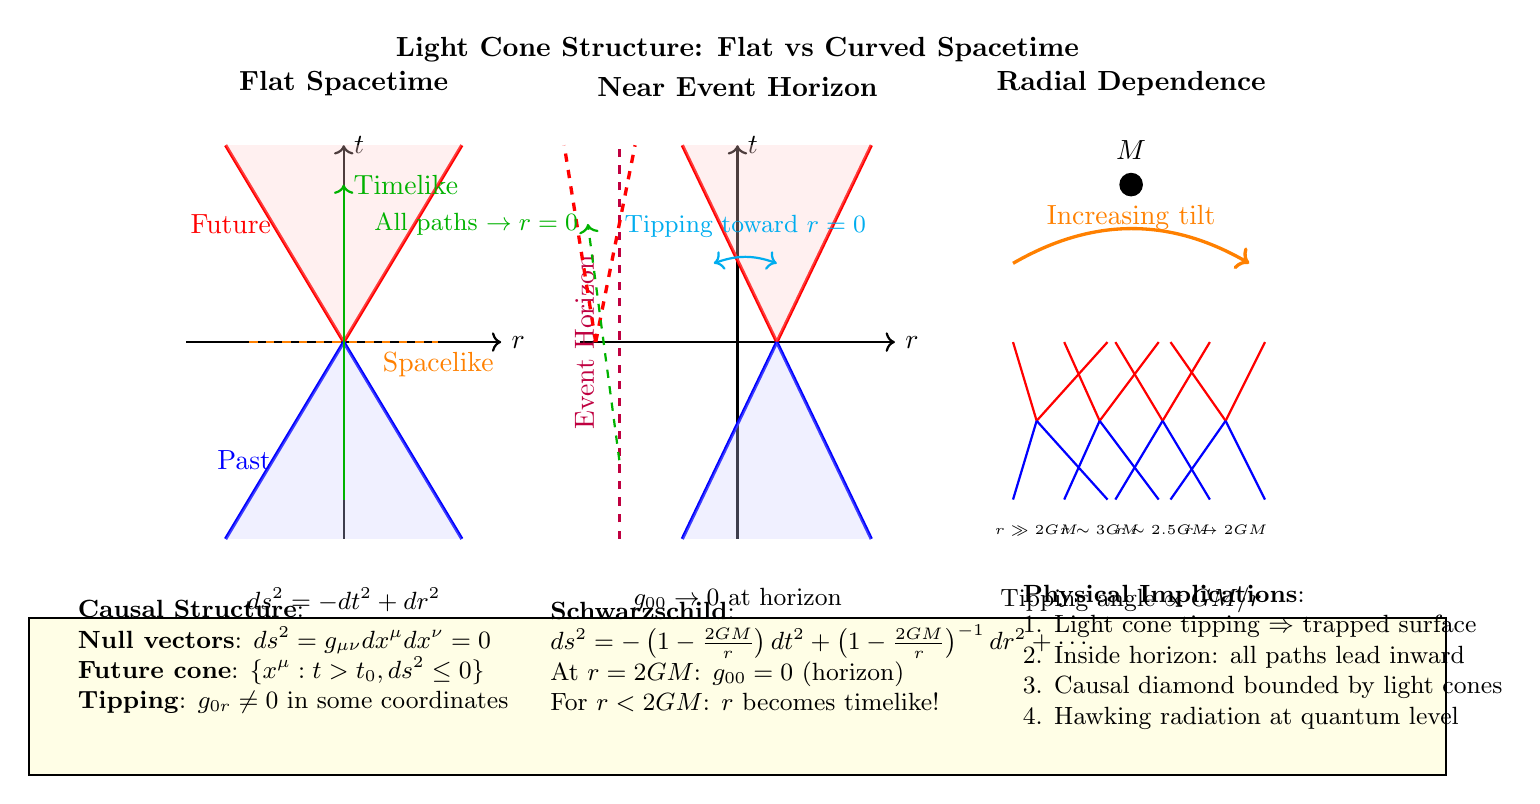
\begin{tikzpicture}[scale=1.0]
    % Title
    \node[anchor=north] at (0,6.5) {\textbf{Light Cone Structure: Flat vs Curved Spacetime}};
    
    % Left: Flat spacetime (Minkowski)
    \begin{scope}[xshift=-5cm]
        \node[above] at (0,5.5) {\textbf{Flat Spacetime}};
        
        % Axes
        \draw[->, thick] (0,0) -- (0,5) node[right] {$t$};
        \draw[->, thick] (-2,2.5) -- (2,2.5) node[right] {$r$};
        
        % Future light cone (symmetric)
        \draw[red, very thick] (0,2.5) -- (-1.5,5);
        \draw[red, very thick] (0,2.5) -- (1.5,5);
        \fill[red!20, opacity=0.3] (0,2.5) -- (-1.5,5) -- (1.5,5) -- cycle;
        
        % Past light cone (symmetric)
        \draw[blue, very thick] (0,2.5) -- (-1.5,0);
        \draw[blue, very thick] (0,2.5) -- (1.5,0);
        \fill[blue!20, opacity=0.3] (0,2.5) -- (-1.5,0) -- (1.5,0) -- cycle;
        
        % Time-like worldline
        \draw[->, green!70!black, thick] (0,0.5) -- (0,4.5);
        \node[green!70!black, right] at (0,4.5) {Timelike};
        
        % Space-like
        \draw[orange, thick, dashed] (-1.2,2.5) -- (1.2,2.5);
        \node[orange, below] at (1.2,2.5) {Spacelike};
        
        % Annotations
        \node[red, left] at (-0.8,4.0) {Future};
        \node[blue, left] at (-0.8,1.0) {Past};
        \node[below, align=center, font=\small] at (0,-0.5) {
            $ds^2 = -dt^2 + dr^2$\\
            Symmetric, unchanging
        };
    \end{scope}
    
    % Center: Schwarzschild near horizon
    \begin{scope}[xshift=0cm]
        \node[above] at (0,5.5) {\textbf{Near Event Horizon}};
        
        % Axes
        \draw[->, thick] (0,0) -- (0,5) node[right] {$t$};
        \draw[->, thick] (-2,2.5) -- (2,2.5) node[right] {$r$};
        
        % Event horizon (vertical dashed line)
        \draw[purple, very thick, dashed] (-1.5,0) -- (-1.5,5);
        \node[purple, above, rotate=90] at (-1.7,2.5) {Event Horizon};
        
        % Tipped light cone at r > 2GM
        \draw[red, very thick] (0.5,2.5) -- (-0.7,5);
        \draw[red, very thick] (0.5,2.5) -- (1.7,5);
        \fill[red!20, opacity=0.3] (0.5,2.5) -- (-0.7,5) -- (1.7,5) -- cycle;
        
        % Past cone (also tipped)
        \draw[blue, very thick] (0.5,2.5) -- (-0.7,0);
        \draw[blue, very thick] (0.5,2.5) -- (1.7,0);
        \fill[blue!20, opacity=0.3] (0.5,2.5) -- (-0.7,0) -- (1.7,0) -- cycle;
        
        % Tipping angle annotation
        \draw[<->, cyan, thick] (0.5,3.5) to[bend right=20] (-0.3,3.5);
        \node[cyan, above, font=\small] at (0.1,3.7) {Tipping toward $r=0$};
        
        % Inside horizon: light cones tip inward
        \draw[red, very thick, dashed] (-1.8,2.5) -- (-2.2,5);
        \draw[red, very thick, dashed] (-1.8,2.5) -- (-1.3,5);
        
        % Worldline forced inward
        \draw[->, green!70!black, thick, dashed] (-1.5,1.0) -- (-1.9,4.0);
        \node[green!70!black, left, font=\small] at (-1.9,4.0) {All paths $\to r=0$};
        
        \node[below, align=center, font=\small] at (0,-0.5) {
            $g_{00} \to 0$ at horizon\\
            Causal structure deformed
        };
    \end{scope}
    
    % Right: Strong field visualization
    \begin{scope}[xshift=5cm]
        \node[above] at (0,5.5) {\textbf{Radial Dependence}};
        
        % Multiple light cones at different radii
        \foreach \x/\tip in {-1.2/0.3, -0.4/0.15, 0.4/0.0, 1.2/-0.1} {
            \draw[red, thick] (\x,1.5) -- (\x-0.6+\tip,2.5);
            \draw[red, thick] (\x,1.5) -- (\x+0.6+\tip,2.5);
            \draw[blue, thick] (\x,1.5) -- (\x-0.6+\tip,0.5);
            \draw[blue, thick] (\x,1.5) -- (\x+0.6+\tip,0.5);
        }
        
        % Radial coordinate labels
        \node[below, font=\tiny] at (-1.2,0.3) {$r \gg 2GM$};
        \node[below, font=\tiny] at (-0.4,0.3) {$r \sim 3GM$};
        \node[below, font=\tiny] at (0.4,0.3) {$r \sim 2.5GM$};
        \node[below, font=\tiny] at (1.2,0.3) {$r \to 2GM$};
        
        % Tipping progression arrow
        \draw[->, orange, very thick] (-1.5,3.5) to[bend left=30] (1.5,3.5);
        \node[orange, above] at (0,3.8) {Increasing tilt};
        
        % Mass source
        \fill[black] (0,4.5) circle (0.15);
        \node[above] at (0,4.7) {$M$};
        
        \node[below, align=center, font=\small] at (0,-0.5) {
            Tipping angle $\propto GM/r$\\
            Causality preserved
        };
    \end{scope}
    
    % Bottom: Mathematical formulation
    \draw[thick, fill=yellow!10] (-9,-1.0) rectangle (9,-3.0);
    
    \node[align=left, font=\small, anchor=west] at (-8.5,-1.5) {
        \textbf{Causal Structure}:\\
        \textbf{Null vectors}: $ds^2 = g_{\mu\nu}dx^\mu dx^\nu = 0$\\
        \textbf{Future cone}: $\{x^\mu : t > t_0, ds^2 \leq 0\}$\\
        \textbf{Tipping}: $g_{0r} \neq 0$ in some coordinates
    };
    
    \node[align=left, font=\small, anchor=west] at (-2.5,-1.5) {
        \textbf{Schwarzschild}:\\
        $ds^2 = -\left(1-\frac{2GM}{r}\right)dt^2 + \left(1-\frac{2GM}{r}\right)^{-1}dr^2 + \cdots$\\
        At $r = 2GM$: $g_{00} = 0$ (horizon)\\
        For $r < 2GM$: $r$ becomes timelike!
    };
    
    \node[align=left, font=\small, anchor=west] at (3.5,-1.5) {
        \textbf{Physical Implications}:\\
        1. Light cone tipping $\Rightarrow$ trapped surface\\
        2. Inside horizon: all paths lead inward\\
        3. Causal diamond bounded by light cones\\
        4. Hawking radiation at quantum level
    };
    
\end{tikzpicture}
\caption{Light cone structure in curved spacetime. Left: flat Minkowski spacetime with symmetric light cones. Center: near Schwarzschild event horizon showing light cone tipping toward $r=0$, with all worldlines forced inward for $r < 2GM$. Right: radial progression showing increasing tilt as $r \to 2GM$. Bottom: mathematical formulation of causal structure and physical implications for black hole horizons.}
\label{fig:lightcone_curved}
\end{figure}

\caption{Light cone structure: Flat (Minkowski) vs. curved (Schwarzschild). In flat space, light cones are 45° throughout. In curved space near horizon $r = 2GM$, light cones tip progressively inward---at horizon, even radially outward light rays remain at constant $r$. \mphys{Event horizon forms where light cones tip so far that escape becomes impossible.}}
\label{fig:prelim:lightcone-curved}
\end{figure}

Light cones define causal structure: which events can influence which others.

\textbf{Flat spacetime}: Light cones preserve 45° angle everywhere. Causal structure is simple: past light cone defines observable history, future light cone defines influenceable region.

\textbf{Curved spacetime}: Light cones tip due to gravitational time dilation and spatial curvature:
\begin{itemize}
  \item \textbf{Near massive objects}: Light cones tip toward center of mass.
  \item \textbf{At event horizon}: Light cone tips so far that interior/exterior become causally disconnected.
  \item \textbf{Cosmology}: Expanding universe causes light cones to tip due to cosmic expansion.
\end{itemize}

\textbf{Implications}:
\begin{itemize}
  \item GPS signals: Light travel time affected by curvature (Shapiro delay).
  \item Black hole information paradox: Tipped light cones prevent information escape.
  \item Cosmic horizons: Expanding universe creates regions forever beyond causal contact.
\end{itemize}

%-----------------------------------------------------------------------------
% Dimensional Analysis Workflow
%-----------------------------------------------------------------------------

\subsubsection{Dimensional Analysis and Unit Consistency}

\begin{figure}[htbp]
\centering
% Dimensional Analysis Workflow for Chapter 1 Concepts
% Systematic tracking of units through GR calculations
% Essential for verification and physical interpretation

\begin{figure}[htbp]
\centering
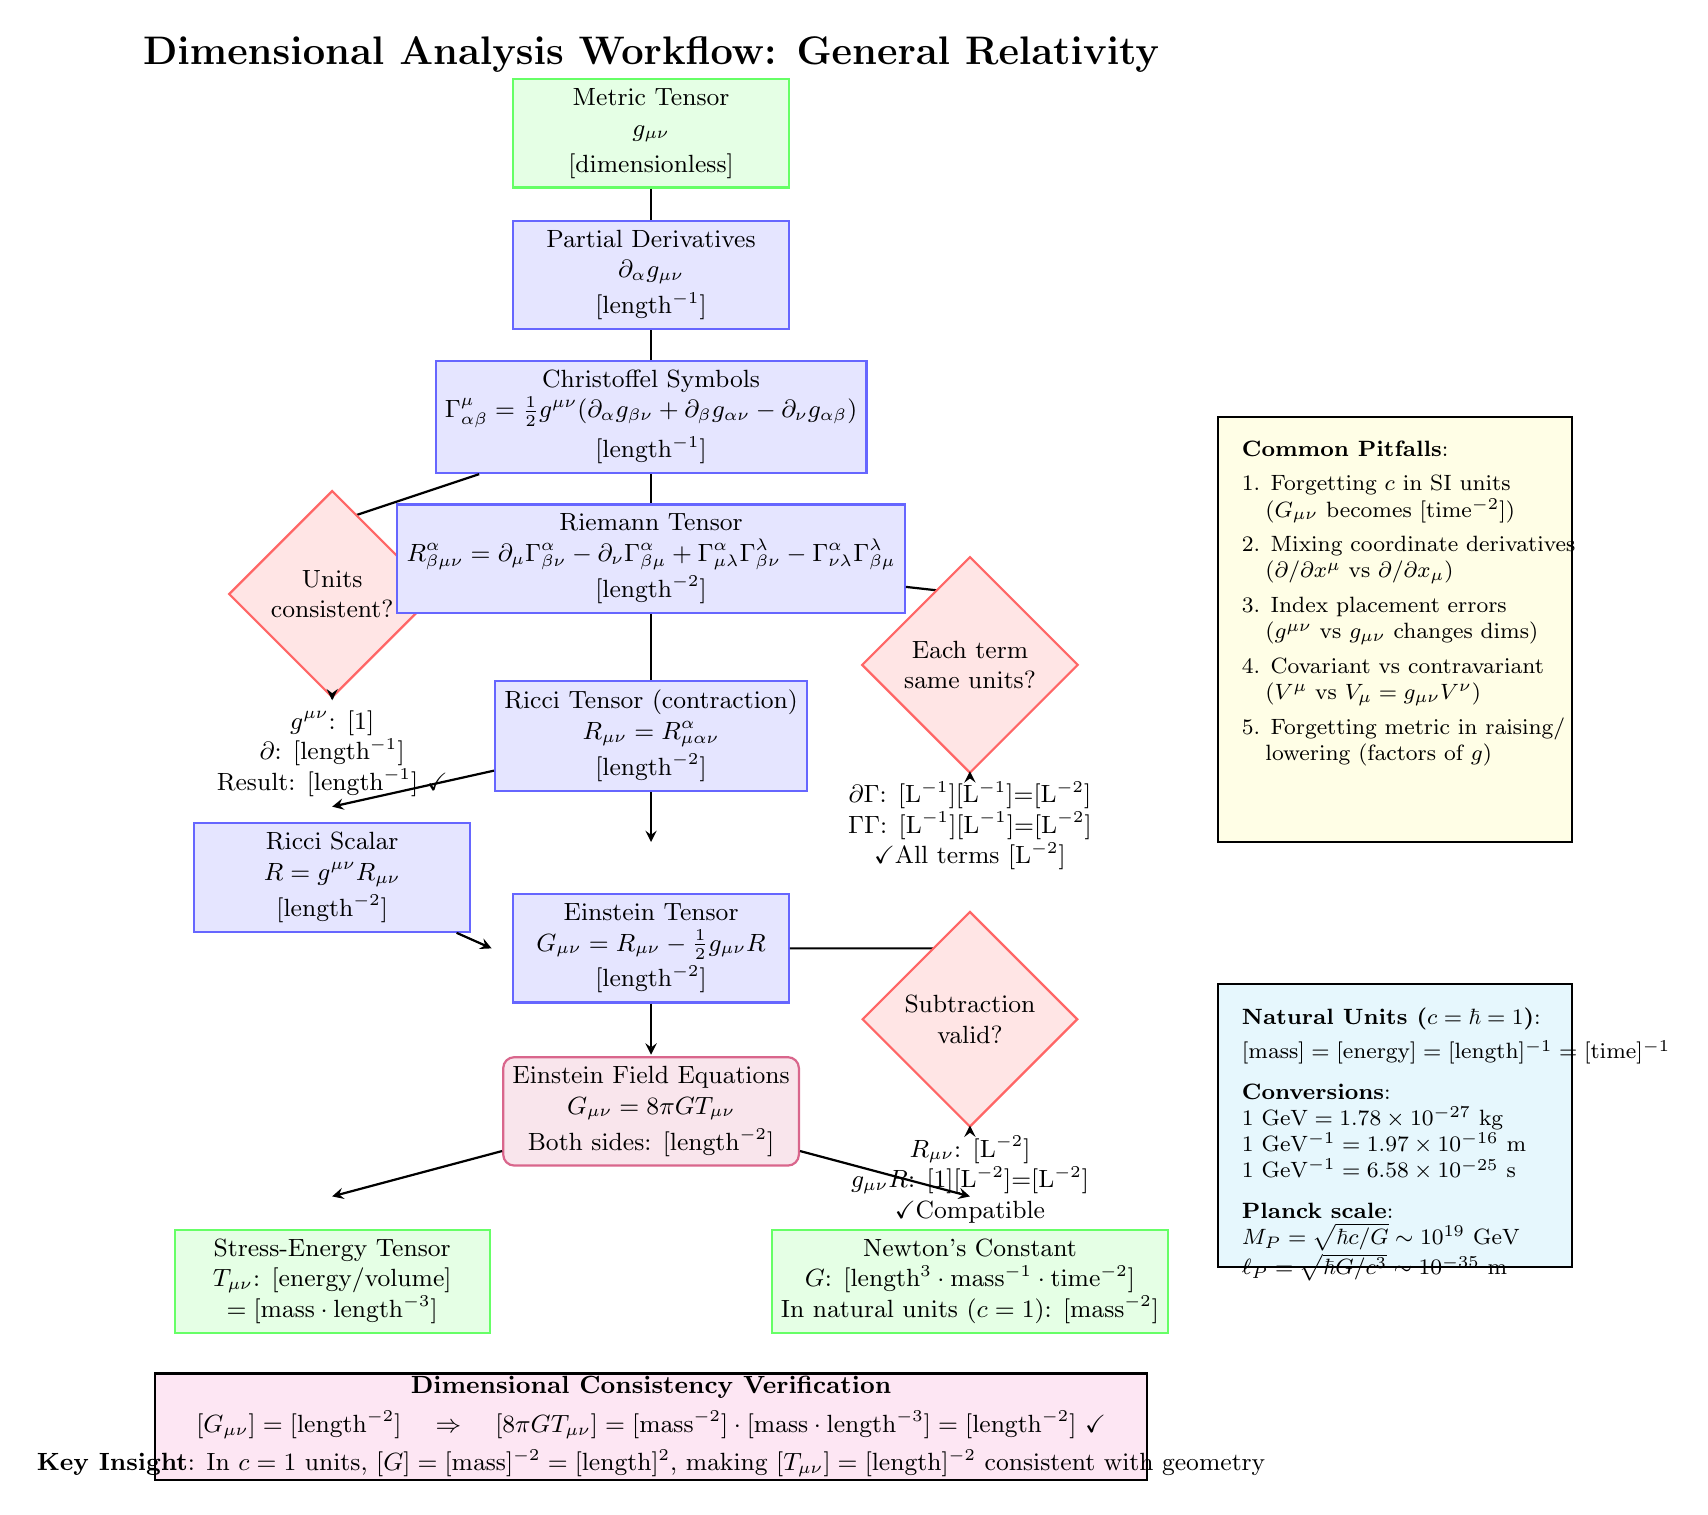
\begin{tikzpicture}[scale=0.9,
    process/.style={rectangle, draw=blue!60, fill=blue!10, thick, minimum width=3.5cm, minimum height=0.9cm, align=center, font=\small},
    data/.style={rectangle, draw=green!60, fill=green!10, thick, minimum width=3.5cm, minimum height=0.7cm, align=center, font=\small},
    check/.style={diamond, draw=red!60, fill=red!10, thick, minimum width=2.5cm, minimum height=0.9cm, align=center, font=\small},
    result/.style={rectangle, draw=purple!60, fill=purple!10, thick, minimum width=3.5cm, minimum height=0.9cm, align=center, font=\small, rounded corners},
    arrow/.style={->, >=stealth, thick}
]

    % Title
    \node[anchor=north, font=\Large\bfseries] at (0,8.5) {Dimensional Analysis Workflow: General Relativity};
    
    % Starting point: Metric
    \node[data] (metric) at (0,7) {Metric Tensor\\$g_{\mu\nu}$\\[2pt][dimensionless]};
    
    % First derivatives
    \draw[arrow] (metric) -- (0,5.5);
    \node[process] (partialg) at (0,5) {Partial Derivatives\\$\partial_\alpha g_{\mu\nu}$\\[2pt]$[\text{length}^{-1}]$};
    
    % Christoffel symbols
    \draw[arrow] (partialg) -- (0,3.5);
    \node[process] (chris) at (0,3) {Christoffel Symbols\\$\Gamma^\mu_{\alpha\beta} = \frac{1}{2}g^{\mu\nu}(\partial_\alpha g_{\beta\nu} + \partial_\beta g_{\alpha\nu} - \partial_\nu g_{\alpha\beta})$\\[2pt]$[\text{length}^{-1}]$};
    
    % Dimensional check 1
    \draw[arrow] (chris) -- (-4.5,1.5);
    \node[check] (check1) at (-4.5,0.5) {Units\\consistent?};
    \draw[arrow] (check1) -- (-4.5,-1) node[below, font=\small, align=center] {$g^{\mu\nu}$: [1]\\$\partial$: [length$^{-1}$]\\Result: [length$^{-1}$] \checkmark};
    
    % Riemann tensor (parallel path)
    \draw[arrow] (chris) -- (0,1.5);
    \node[process] (riemann) at (0,1) {Riemann Tensor\\$R^\alpha_{\beta\mu\nu} = \partial_\mu \Gamma^\alpha_{\beta\nu} - \partial_\nu \Gamma^\alpha_{\beta\mu} + \Gamma^\alpha_{\mu\lambda}\Gamma^\lambda_{\beta\nu} - \Gamma^\alpha_{\nu\lambda}\Gamma^\lambda_{\beta\mu}$\\[2pt]$[\text{length}^{-2}]$};
    
    % Dimensional check 2
    \draw[arrow] (riemann) -- (4.5,0.5);
    \node[check] (check2) at (4.5,-0.5) {Each term\\same units?};
    \draw[arrow] (check2) -- (4.5,-2) node[below, font=\small, align=center] {$\partial \Gamma$: [L$^{-1}$][L$^{-1}$]=[L$^{-2}$]\\$\Gamma \Gamma$: [L$^{-1}$][L$^{-1}$]=[L$^{-2}$]\\\checkmark All terms [L$^{-2}$]};
    
    % Ricci tensor
    \draw[arrow] (riemann) -- (0,-1);
    \node[process] (ricci) at (0,-1.5) {Ricci Tensor (contraction)\\$R_{\mu\nu} = R^\alpha_{\mu\alpha\nu}$\\[2pt]$[\text{length}^{-2}]$};
    
    % Ricci scalar
    \draw[arrow] (ricci) -- (-4.5,-2.5);
    \node[process] (scalar) at (-4.5,-3.5) {Ricci Scalar\\$R = g^{\mu\nu}R_{\mu\nu}$\\[2pt]$[\text{length}^{-2}]$};
    
    % Einstein tensor
    \draw[arrow] (ricci) -- (0,-3);
    \draw[arrow] (scalar) -- (-2.25,-4.5);
    \node[process] (einstein) at (0,-4.5) {Einstein Tensor\\$G_{\mu\nu} = R_{\mu\nu} - \frac{1}{2}g_{\mu\nu}R$\\[2pt]$[\text{length}^{-2}]$};
    
    % Dimensional check 3
    \draw[arrow] (einstein) -- (4.5,-4.5);
    \node[check] (check3) at (4.5,-5.5) {Subtraction\\valid?};
    \draw[arrow] (check3) -- (4.5,-7) node[below, font=\small, align=center] {$R_{\mu\nu}$: [L$^{-2}$]\\$g_{\mu\nu}R$: [1][L$^{-2}$]=[L$^{-2}$]\\\checkmark Compatible};
    
    % Field equations
    \draw[arrow] (einstein) -- (0,-6);
    \node[result] (field) at (0,-6.8) {Einstein Field Equations\\$G_{\mu\nu} = 8\pi G T_{\mu\nu}$\\[2pt]Both sides: $[\text{length}^{-2}]$};
    
    % Stress-energy check
    \draw[arrow] (field) -- (-4.5,-8);
    \node[data, minimum width=4cm] (stress) at (-4.5,-9.2) {Stress-Energy Tensor\\$T_{\mu\nu}$: $[\text{energy}/\text{volume}]$\\$= [\text{mass} \cdot \text{length}^{-3}]$};
    
    % Gravitational constant
    \draw[arrow] (field) -- (4.5,-8);
    \node[data, minimum width=4cm] (gravconst) at (4.5,-9.2) {Newton's Constant\\$G$: $[\text{length}^3 \cdot \text{mass}^{-1} \cdot \text{time}^{-2}]$\\In natural units ($c=1$): $[\text{mass}^{-2}]$};
    
    % Final verification box
    \draw[thick, fill=magenta!10] (-7,-10.5) rectangle (7,-12);
    \node[align=center, font=\small] at (0,-11.25) {
        \textbf{Dimensional Consistency Verification}\\[3pt]
        $[G_{\mu\nu}] = [\text{length}^{-2}]$ \quad $\Rightarrow$ \quad $[8\pi G T_{\mu\nu}] = [\text{mass}^{-2}] \cdot [\text{mass} \cdot \text{length}^{-3}] = [\text{length}^{-2}]$ \checkmark\\[3pt]
        \textbf{Key Insight}: In $c=1$ units, $[G] = [\text{mass}]^{-2} = [\text{length}]^2$, making $[T_{\mu\nu}] = [\text{length}]^{-2}$ consistent with geometry
    };
    
    % Side annotation box: Common pitfalls
    \draw[thick, fill=yellow!10] (8,3) rectangle (13,-3);
    \node[align=left, font=\footnotesize, anchor=north west] at (8.2,2.8) {
        \textbf{Common Pitfalls}:\\[3pt]
        1. Forgetting $c$ in SI units\\
        \quad $(G_{\mu\nu}$ becomes $[\text{time}^{-2}])$\\[3pt]
        2. Mixing coordinate derivatives\\
        \quad $(\partial/\partial x^\mu$ vs $\partial/\partial x_\mu)$\\[3pt]
        3. Index placement errors\\
        \quad $(g^{\mu\nu}$ vs $g_{\mu\nu}$ changes dims)\\[3pt]
        4. Covariant vs contravariant\\
        \quad $(V^\mu$ vs $V_\mu = g_{\mu\nu}V^\nu)$\\[3pt]
        5. Forgetting metric in raising/\\
        \quad lowering (factors of $g$)
    };
    
    % Side annotation box: Natural units
    \draw[thick, fill=cyan!10] (8,-5) rectangle (13,-9);
    \node[align=left, font=\footnotesize, anchor=north west] at (8.2,-5.2) {
        \textbf{Natural Units ($c=\hbar=1$)}:\\[3pt]
        $[\text{mass}] = [\text{energy}] = [\text{length}]^{-1} = [\text{time}]^{-1}$\\[5pt]
        \textbf{Conversions}:\\
        $1 \text{ GeV} = 1.78 \times 10^{-27}$ kg\\
        $1 \text{ GeV}^{-1} = 1.97 \times 10^{-16}$ m\\
        $1 \text{ GeV}^{-1} = 6.58 \times 10^{-25}$ s\\[5pt]
        \textbf{Planck scale}:\\
        $M_P = \sqrt{\hbar c/G} \sim 10^{19}$ GeV\\
        $\ell_P = \sqrt{\hbar G/c^3} \sim 10^{-35}$ m
    };
    
\end{tikzpicture}
\caption{Dimensional analysis workflow for general relativity calculations. Main flow (center): systematic progression from metric tensor through Christoffel symbols, Riemann tensor, Ricci tensor/scalar, Einstein tensor, to field equations, with dimensional consistency checks at each stage. Right boxes: common pitfalls to avoid and natural unit conversions. All tensor components track dimensions explicitly to ensure physical consistency.}
\label{fig:dimensional_analysis}
\end{figure}

\caption{Dimensional analysis workflow: Metric $\to$ Christoffel $\to$ Riemann $\to$ Einstein equations. At each stage, verify dimensional consistency: $[g_{\mu\nu}] = \text{dimensionless}$, $[\Gamma^\rho_{\mu\nu}] = [\text{length}]^{-1}$, $[R^\rho{}_{\sigma\mu\nu}] = [\text{length}]^{-2}$, $[G_{\mu\nu}] = [\text{length}]^{-2}$. \mcaution{Common error: forgetting factor of $c^2$ in $T_{\mu\nu}$ conversion between geometrized units and SI.}}
\label{fig:prelim:dimensional-analysis}
\end{figure}

\textbf{Three key dimensional checks}:

\textbf{1. Metric and Christoffel consistency}:
\begin{equation}
  \Gamma^\rho_{\mu\nu} = \frac{1}{2} g^{\rho\sigma} (\partial_\mu g_{\nu\sigma} + \partial_\nu g_{\mu\sigma} - \partial_\sigma g_{\mu\nu})
\end{equation}
\begin{itemize}
  \item $[g_{\mu\nu}] = \text{dimensionless}$ (in geometrized units).
  \item $[\partial_\mu] = [\text{length}]^{-1}$ (derivative is inverse length).
  \item $[\Gamma^\rho_{\mu\nu}] = [\text{length}]^{-1}$ (consistent).
\end{itemize}

\textbf{2. Riemann curvature}:
\begin{equation}
  R^\rho{}_{\sigma\mu\nu} = \partial_\mu \Gamma^\rho_{\nu\sigma} - \partial_\nu \Gamma^\rho_{\mu\sigma} + \Gamma^\rho_{\mu\lambda} \Gamma^\lambda_{\nu\sigma} - \Gamma^\rho_{\nu\lambda} \Gamma^\lambda_{\mu\sigma}
\end{equation}
\begin{itemize}
  \item $[\partial_\mu \Gamma] = [\text{length}]^{-1} \times [\text{length}]^{-1} = [\text{length}]^{-2}$ ✓
  \item $[\Gamma \times \Gamma] = [\text{length}]^{-1} \times [\text{length}]^{-1} = [\text{length}]^{-2}$ ✓
  \item $[R^\rho{}_{\sigma\mu\nu}] = [\text{length}]^{-2}$ (intrinsic curvature scale).
\end{itemize}

\textbf{3. Einstein field equations}:
\begin{equation}
  G_{\mu\nu} = \frac{8\pi G}{c^4} T_{\mu\nu}
\end{equation}
\begin{itemize}
  \item $[G_{\mu\nu}] = [R_{\mu\nu}] = [\text{length}]^{-2}$.
  \item $[T_{\mu\nu}] = [\text{energy}]/[\text{volume}] = [\text{mass}][\text{length}]^{-1}[\text{time}]^{-2}$.
  \item $[8\pi G/c^4] = [\text{length}][\text{mass}]^{-1} \times [\text{time}]^{-4}[\text{length}]^{-4} = [\text{mass}]^{-1}[\text{time}]^{-4}[\text{length}]^{-3}$.
  \item Combined: $[G/c^4 \times T] = [\text{length}]^{-2}$ ✓ (consistent with $[G_{\mu\nu}]$).
\end{itemize}

\textbf{Common pitfalls}:
\begin{itemize}
  \item \textbf{Natural units confusion}: Setting $c = G = \hbar = 1$ hides dimensional factors. Always restore units for physical predictions.
  \item \textbf{Signature conventions}: Some texts use $(+,-,-,-)$ signature, affecting signs in equations.
  \item \textbf{Index placement}: Upper vs. lower indices affect dimensions when metric is not dimensionless.
\end{itemize}

%-----------------------------------------------------------------------------
% Comprehensive Reference Tables: Special Cases, Computational Complexity, etc.
%-----------------------------------------------------------------------------

\subsubsection{Comprehensive Reference: Special Cases and Regimes}

% Special Cases and Limiting Behaviors in General Relativity
% Comprehensive comparison across different spacetime geometries
% Essential reference for understanding when approximations are valid

\begin{table}[htbp]
\centering
\caption{Special Cases and Limiting Behaviors in General Relativity}
\label{tab:special_cases_gr}
\begin{tabular}{|l|l|p{5cm}|p{4cm}|p{3.5cm}|}
\hline
\textbf{Case} & \textbf{Condition} & \textbf{Metric/Key Feature} & \textbf{Physical System} & \textbf{Validity} \\
\hline
\hline
\multicolumn{5}{|c|}{\textbf{Flat Spacetime}} \\
\hline
Minkowski & $R_{\mu\nu\alpha\beta} = 0$ & $ds^2 = -dt^2 + dx^2 + dy^2 + dz^2$ & Special relativity, no gravity & Exact in absence of matter \\
\hline
\hline
\multicolumn{5}{|c|}{\textbf{Weak Field Approximations}} \\
\hline
Newtonian limit & $|g_{\mu\nu} - \eta_{\mu\nu}| \ll 1$, $v \ll c$ & $g_{00} \approx -(1 + 2\Phi/c^2)$ where $\nabla^2\Phi = 4\pi G\rho$ & Solar system orbits, GPS corrections & $GM/rc^2 \ll 1$ and $v \ll c$ \\
\hline
Post-Newtonian & $|h_{\mu\nu}| \sim (v/c)^2$ & $g_{\mu\nu} = \eta_{\mu\nu} + h_{\mu\nu} + O(v^4/c^4)$ & Binary pulsars, precision tests & $(v/c)^2 \sim 10^{-4}$ to $10^{-1}$ \\
\hline
Linearized GR & $|h_{\mu\nu}| \ll 1$ & $\Box h_{\mu\nu} = -16\pi G T_{\mu\nu}$ (wave equation) & Gravitational waves far from source & Strain $h \sim 10^{-21}$ (LIGO) \\
\hline
\hline
\multicolumn{5}{|c|}{\textbf{Spherically Symmetric Solutions}} \\
\hline
Schwarzschild & $T_{\mu\nu} = 0$, static, spherical & $ds^2 = -(1-\frac{2GM}{r})dt^2 + (1-\frac{2GM}{r})^{-1}dr^2 + r^2 d\Omega^2$ & Non-rotating black hole, star exterior & Exact vacuum solution \\
\hline
Schwarzschild interior & $\rho = \text{const}$, $p = p(r)$ & Matches to Schwarzschild at surface $R$ & Constant density star (crude approx) & $R > \frac{9}{4}r_s$ (stability) \\
\hline
Reissner-Nordstrom & $T_{\mu\nu} = F_{\mu\alpha}F_\nu^\alpha$, charge $Q$ & Additional $+\frac{GQ^2}{r^2}$ term in $g_{00}$ & Charged black hole & Exact for $Q \neq 0$, $J=0$ \\
\hline
\hline
\multicolumn{5}{|c|}{\textbf{Rotating Solutions}} \\
\hline
Kerr & $T_{\mu\nu} = 0$, stationary, axisymmetric & Frame dragging $g_{t\phi} \neq 0$, ergosphere, ring singularity & Rotating black hole, pulsars & Exact for $a = J/M < M$ \\
\hline
Kerr-Newman & Charge $Q$ and angular momentum $J$ & Combines Reissner-Nordstrom and Kerr & Rotating charged black hole & Most general stationary BH \\
\hline
\hline
\multicolumn{5}{|c|}{\textbf{Cosmological Solutions}} \\
\hline
FLRW (flat) & Homogeneous, isotropic, $k=0$ & $ds^2 = -dt^2 + a(t)^2(dx^2 + dy^2 + dz^2)$ & Standard cosmology ($\Omega_{\text{tot}} = 1$) & $\Lambda$CDM for $a \propto t^{2/3}$ (matter era) \\
\hline
FLRW (closed) & $k = +1$ & $ds^2 = -dt^2 + a(t)^2\frac{dr^2}{1-r^2} + \cdots$ & Closed universe ($\Omega > 1$) & Recollapses if no dark energy \\
\hline
FLRW (open) & $k = -1$ & $ds^2 = -dt^2 + a(t)^2\frac{dr^2}{1+r^2} + \cdots$ & Open universe ($\Omega < 1$) & Expands forever \\
\hline
de Sitter & $T_{\mu\nu} = 0$, $\Lambda > 0$ & $ds^2 = -(1-\frac{r^2}{R^2})dt^2 + (1-\frac{r^2}{R^2})^{-1}dr^2 + \cdots$, $R = \sqrt{3/\Lambda}$ & Pure vacuum energy (inflation, late-time acceleration) & Exact for $\rho = 0$, $\Lambda \neq 0$ \\
\hline
Anti-de Sitter & $\Lambda < 0$ & Negative curvature everywhere & AdS/CFT correspondence (string theory) & Conformal boundary \\
\hline
\hline
\multicolumn{5}{|c|}{\textbf{Wave-like Solutions}} \\
\hline
pp-waves & $T_{\mu\nu} = 0$, plane-fronted & $ds^2 = -2du\,dv + H(u,x,y)du^2 + dx^2 + dy^2$ & Gravitational wave (exact) & Penrose limit of any spacetime \\
\hline
TT gauge & $h_{ij}^{TT}$, transverse-traceless & $h_{+} = A \cos(\omega(t-z))$, $h_{\times} = A \sin(\omega(t-z))$ & LIGO/Virgo detections & Far from source, $r \gg \lambda$ \\
\hline
\hline
\multicolumn{5}{|c|}{\textbf{Strong Field Regimes}} \\
\hline
Near horizon ($r \to 2GM$) & $g_{00} \to 0$ & Light cone tipping, infinite redshift & Black hole physics, Hawking radiation & Quantum effects at $r \sim r_s$ \\
\hline
Planck scale & $\ell \sim \ell_P = \sqrt{\hbar G/c^3}$ & GR breaks down, quantum gravity needed & Early universe ($t < 10^{-43}$ s), singularities & $\ell_P \sim 10^{-35}$ m \\
\hline
\hline
\multicolumn{5}{|c|}{\textbf{Specialized Coordinates}} \\
\hline
Rindler & Uniformly accelerating observer & $ds^2 = -(a\xi)^2 dt^2 + d\xi^2 + dy^2 + dz^2$ & Unruh effect, acceleration horizons & Minkowski in disguise \\
\hline
Kruskal-Szekeres & Maximal extension of Schwarzschild & Regular at horizon, shows two exterior regions & Black/white hole, wormhole (traversable?) & Covers full Schwarzschild manifold \\
\hline
Eddington-Finkelstein & Ingoing/outgoing null coordinates & Regular at horizon for infalling matter & Gravitational collapse & Preferred for dynamics \\
\hline
\end{tabular}
\end{table}

\begin{table}[htbp]
\centering
\caption{Parameter Regimes and Characteristic Scales}
\label{tab:parameter_regimes}
\begin{tabular}{|l|c|l|p{6cm}|}
\hline
\textbf{Regime} & \textbf{Dimensionless Parameter} & \textbf{Typical Value} & \textbf{Physical Systems \& Observables} \\
\hline
\hline
Weak field & $\epsilon = \frac{GM}{rc^2}$ & $\epsilon \ll 1$ & \textbullet~Solar system: $\epsilon \sim 10^{-6}$ (Earth orbit) \newline \textbullet~GPS satellites: $\epsilon \sim 10^{-9}$ \newline \textbullet~Perihelion precession: $\sim \epsilon$ per orbit \\
\hline
Strong field & $\epsilon = \frac{GM}{rc^2}$ & $\epsilon \sim 0.1 - 0.5$ & \textbullet~Neutron star surface: $\epsilon \sim 0.2$ \newline \textbullet~Event horizon: $\epsilon = 0.5$ \newline \textbullet~Light bending: $\Delta\theta \sim 2\epsilon$ \\
\hline
Post-Newtonian & $v/c$ & $10^{-4} < v/c < 10^{-1}$ & \textbullet~Binary pulsars: $v/c \sim 10^{-3}$ \newline \textbullet~BH mergers (LIGO): $v/c \sim 0.3 - 0.6$ \newline \textbullet~Corrections: $O((v/c)^2, (v/c)^4, \ldots)$ \\
\hline
Cosmological & $H_0^{-1}$ (Hubble time) & $\sim 14$ Gyr & \textbullet~CMB anisotropies: $\Delta T/T \sim 10^{-5}$ \newline \textbullet~Dark energy: $\rho_\Lambda/\rho_c \sim 0.7$ \newline \textbullet~Curvature: $|k| < 0.01$ (flat) \\
\hline
GW strain & $h = \frac{\Delta L}{L}$ & $10^{-23} < h < 10^{-21}$ & \textbullet~LIGO sensitivity: $h \sim 10^{-23}$ \newline \textbullet~Binary coalescence: $h \sim 10^{-21}$ at 100 Mpc \newline \textbullet~Stochastic background: $\Omega_{GW} \sim 10^{-15}$ \\
\hline
Quantum gravity & $\ell/\ell_P$ & $\ell \gg \ell_P$ (classical) & \textbullet~Planck length: $\ell_P \sim 10^{-35}$ m \newline \textbullet~Planck energy: $E_P \sim 10^{19}$ GeV \newline \textbullet~Black hole evaporation: $t \sim (M/M_P)^3 t_P$ \\
\hline
Compactness & $\mathcal{C} = \frac{GM}{Rc^2}$ & $\mathcal{C} < 0.5$ (stable) & \textbullet~Sun: $\mathcal{C} \sim 10^{-6}$ \newline \textbullet~White dwarf: $\mathcal{C} \sim 10^{-4}$ \newline \textbullet~Neutron star: $\mathcal{C} \sim 0.2$ \newline \textbullet~Black hole: $\mathcal{C} = 0.5$ (horizon) \\
\hline
\end{tabular}
\end{table}

\begin{table}[htbp]
\centering
\caption{Approximation Validity and Corrections}
\label{tab:approximation_corrections}
\begin{tabular}{|l|p{7cm}|p{7cm}|}
\hline
\textbf{Approximation} & \textbf{Leading Correction} & \textbf{When Breakdown Occurs} \\
\hline
\hline
Newtonian gravity & Post-Newtonian: $O((v/c)^2, GM/rc^2)$ & $v/c > 0.1$ or $GM/rc^2 > 0.01$ (strong field or high velocity) \\
\hline
Special relativity (no gravity) & GR corrections: $\Delta t/t \sim GM/rc^2$ & Any gravitational field, e.g., GPS ($\Delta t \sim 38$ $\mu$s/day) \\
\hline
Schwarzschild (non-rotating) & Kerr (rotation): $a/M = J/M^2$ & Rotating objects (all realistic astrophysical sources) \\
\hline
Schwarzschild (uncharged) & Reissner-Nordstrom: $Q^2 G/c^4 M^2$ & Charged black holes (ratio $Q/M \ll 1$ in nature) \\
\hline
Weak field linearized GR & Quadratic corrections: $O(h^2)$ & $h > 10^{-2}$ (strong field near compact objects) \\
\hline
Geodesic motion (test particle) & Self-force: $m/M$ & Extended objects, tidal deformation ($m/M > 10^{-6}$) \\
\hline
Vacuum Einstein equations & Matter stress-energy: $8\pi G T_{\mu\nu}/c^4$ & Any matter present (stars, gas, radiation) \\
\hline
Point-particle approximation & Tidal forces: $R_{\mu\nu\alpha\beta} \times (\text{size})^2$ & Object size comparable to curvature radius \\
\hline
Slow-motion ($v \ll c$) & Relativistic corrections: $(v/c)^2$ & High velocities (e.g., particle accelerators, BH mergers) \\
\hline
Static spacetime & Time-dependent: $\partial_t g_{\mu\nu} \neq 0$ & Gravitational waves, cosmological expansion, collapse \\
\hline
Asymptotic flatness & Cosmological constant: $\Lambda r^2$ & Large distances ($r > \Lambda^{-1/2} \sim 10^{26}$ m for $\Lambda_{\text{obs}}$) \\
\hline
Classical GR & Quantum corrections: $\hbar G E^2/c^5$ & Planck scale energies ($E \sim 10^{19}$ GeV), black hole evaporation \\
\hline
\end{tabular}
\end{table}


\mex{Schwarzschild solution: Weak field ($GM/rc^2 \ll 1$, Solar System), strong field ($GM/rc^2 \sim 1$, neutron stars), extreme ($GM/rc^2 \to 1$, black hole horizons).}

\subsubsection{Computational Complexity and Tools}

% Computational Complexity Comparison Table
% File: tab_computational_complexity.tex
% Purpose: Compare algorithmic complexity for computing GR tensors and provide guidance
% For: Chapter 1 - Mathematical Preliminaries

\begin{table}[htbp]
\centering
\caption{Computational complexity for calculating general relativity tensors from metric $g_{\mu\nu}$ in $D$ spacetime dimensions. Symmetries exploited for component counts. Symbolic computation strongly recommended for $D \geq 4$.}
\label{tab:computational_complexity}
\small
\begin{tabular}{lccccp{4.5cm}}
\toprule
\textbf{Quantity} & \textbf{Components} & \textbf{Operations} & \textbf{Complexity} & \textbf{Symmetry} & \textbf{Notes} \\
\midrule
\multicolumn{6}{l}{\textit{\textbf{Basic Quantities}}} \\
Metric $g_{\mu\nu}$ & $D(D+1)/2$ & -- & -- & Symmetric & Input \\
Inverse $g^{\mu\nu}$ & $D(D+1)/2$ & $O(D^3)$ & Cubic & Matrix inversion & LU decomposition \\
Determinant $\sqrt{-g}$ & 1 & $O(D^3)$ & Cubic & -- & From inversion \\
\midrule
\multicolumn{6}{l}{\textit{\textbf{Connection}}} \\
Partials $\partial_\alpha g_{\mu\nu}$ & $D^2(D+1)/2$ & $O(D^3)$ & Cubic & Symbolic/numeric & Differentiation \\
Christoffel $\Gamma^\mu_{\alpha\beta}$ & $D^2(D+1)/2$ & $O(D^4)$ & Quartic & Symmetric in $\alpha\beta$ & $40$ ind. in 4D \\
\midrule
\multicolumn{6}{l}{\textit{\textbf{Curvature}}} \\
Riemann $R^\alpha_{\beta\mu\nu}$ & $D^2(D^2-1)/12$ & $O(D^5)$ & Quintic & 4 symmetries & $20$ ind. in 4D \\
Ricci $R_{\mu\nu}$ & $D(D+1)/2$ & $O(D^5)$ & Quintic & Contraction & $10$ ind. in 4D \\
Ricci scalar $R$ & 1 & $O(D^5)$ & Quintic & Full contraction & Single value \\
Einstein $G_{\mu\nu}$ & $D(D+1)/2$ & $O(D^5)$ & Quintic & Symmetric & $10$ ind. in 4D \\
\midrule
\multicolumn{6}{l}{\textit{\textbf{Dimensional Examples}}} \\
$D=2$ (surfaces) & $R: 1$ ind. & $O(32)$ & Low & Gauss curvature & Analytically tractable \\
$D=3$ (spatial) & $R: 6$ ind. & $O(243)$ & Moderate & $\Gamma: 18$, $R: 6$ & Feasible by hand \\
$D=4$ (spacetime) & $R: 20$ ind. & $O(1024)$ & High & $\Gamma: 40$, $R: 20$ & Symbolic essential \\
$D=11$ (M-theory) & $R: 1540$ ind. & $O(10^5)$ & Extreme & $\Gamma: 726$, $R: 1540$ & Computational only \\
\midrule
\multicolumn{6}{l}{\textit{\textbf{Optimization Strategies}}} \\
\multicolumn{6}{l}{1. \textbf{Symmetry exploitation}: Reduce components using index symmetries before calculation} \\
\multicolumn{6}{l}{2. \textbf{Symbolic computation}: Use CAS (Mathematica, Maple, SymPy, Cadabra) for $D \geq 4$} \\
\multicolumn{6}{l}{3. \textbf{Coordinate choice}: Select coordinates that simplify metric (diagonal, block-diagonal)} \\
\multicolumn{6}{l}{4. \textbf{Killing vectors}: Exploit spacetime symmetries to reduce independent components} \\
\multicolumn{6}{l}{5. \textbf{Tetrad formalism}: Use orthonormal frames to simplify non-diagonal metrics} \\
\multicolumn{6}{l}{6. \textbf{Numerical methods}: For specific metrics, numerical differentiation faster than symbolic} \\
\bottomrule
\end{tabular}
\end{table}

% Second table: Software tools comparison
\begin{table}[htbp]
\centering
\caption{Software tools for general relativity calculations with features and typical use cases.}
\label{tab:gr_software_tools}
\small
\begin{tabular}{llp{5cm}p{3.5cm}}
\toprule
\textbf{Tool} & \textbf{Type} & \textbf{Strengths} & \textbf{Typical Use} \\
\midrule
\textbf{Mathematica} & Commercial CAS & Full symbolic+numeric, notebooks, visualization & Research, teaching \\
\textbf{Maple} & Commercial CAS & GRTensorII package, symbolic manipulation & Metric calculations \\
\textbf{SymPy} & Python library & Free, programmable, extensible & Automated workflows \\
\textbf{Cadabra} & Specialized & Tensor symmetries, field theory, efficient & Advanced research \\
\textbf{SageMath} & Open CAS & Manifolds package, differential geometry & Teaching, research \\
\textbf{xAct/xTensor} & Mathematica & Abstract index notation, efficiency & Theoretical research \\
\textbf{GRworkbench} & MATLAB & Numerical, visualization, educational & Applied problems \\
\midrule
\multicolumn{4}{l}{\textit{\textbf{Performance Comparison (Schwarzschild metric, $D=4$)}}} \\
Metric $\to$ Christoffel & -- & $<1$ sec (all tools) & Fast \\
Christoffel $\to$ Riemann & -- & $<5$ sec (symbolic) & Moderate \\
Riemann $\to$ Einstein & -- & $<10$ sec (symbolic) & Complex \\
Full chain (metric $\to$ Einstein) & -- & $10-30$ sec (optimized) & Typical workflow \\
\bottomrule
\end{tabular}
\end{table}

% Third table: Algorithmic approaches
\begin{table}[htbp]
\centering
\caption{Algorithmic approaches for computing curvature tensors with trade-offs.}
\label{tab:curvature_algorithms}
\small
\begin{tabular}{lp{4.5cm}p{4cm}l}
\toprule
\textbf{Method} & \textbf{Description} & \textbf{Advantages} & \textbf{Complexity} \\
\midrule
\textbf{Direct differentiation} & Compute $\partial \Gamma$ directly from definition & Conceptually simple, textbook approach & $O(D^5)$ \\
\textbf{Cartan structure eqs.} & Use differential forms and exterior derivative & Coordinate-independent, elegant & $O(D^5)$ \\
\textbf{Tetrad method} & Orthonormal frames $e^a_\mu$, spin connection & Simplifies non-diagonal metrics & $O(D^5)$ \\
\textbf{Automatic differentiation} & Algorithmic differentiation (forward/reverse mode) & Numerically stable, exact derivatives & $O(D^4)$ \\
\textbf{Finite differences} & Numerical differentiation of $g_{\mu\nu}$ & Fast for specific metrics, approximate & $O(D^3)$ \\
\textbf{Symmetry reduction} & Exploit Killing vectors before calculation & Reduces independent components & Varies \\
\midrule
\multicolumn{4}{l}{\textit{\textbf{Recommended Approach by Context}}} \\
\multicolumn{4}{l}{$\bullet$ \textbf{Teaching}: Direct differentiation (pedagogical clarity)} \\
\multicolumn{4}{l}{$\bullet$ \textbf{Research}: Symbolic CAS with symmetry exploitation (accuracy + efficiency)} \\
\multicolumn{4}{l}{$\bullet$ \textbf{Numerical relativity}: Finite differences or automatic differentiation (speed)} \\
\multicolumn{4}{l}{$\bullet$ \textbf{Exact solutions}: Cartan or tetrad methods (elegance, coordinate freedom)} \\
\bottomrule
\end{tabular}
\end{table}


\mcomp{Recommendation: Use Mathematica/Maple for exact symbolic computation, SymPy for Python integration, xAct for advanced tensor manipulation, numerical methods (finite differences) for strong-field astrophysics.}

\subsubsection{Coordinate Systems: Schwarzschild Comparison}

\begin{figure}[htbp]
\centering
% Schwarzschild Coordinates Comparison
% File: tikz_schwarzschild_coordinates.tex
% Purpose: Visualize multiple coordinate systems on same spacetime geometry
% For: Chapter 1 - Mathematical Preliminaries

\begin{figure}[htbp]
\centering
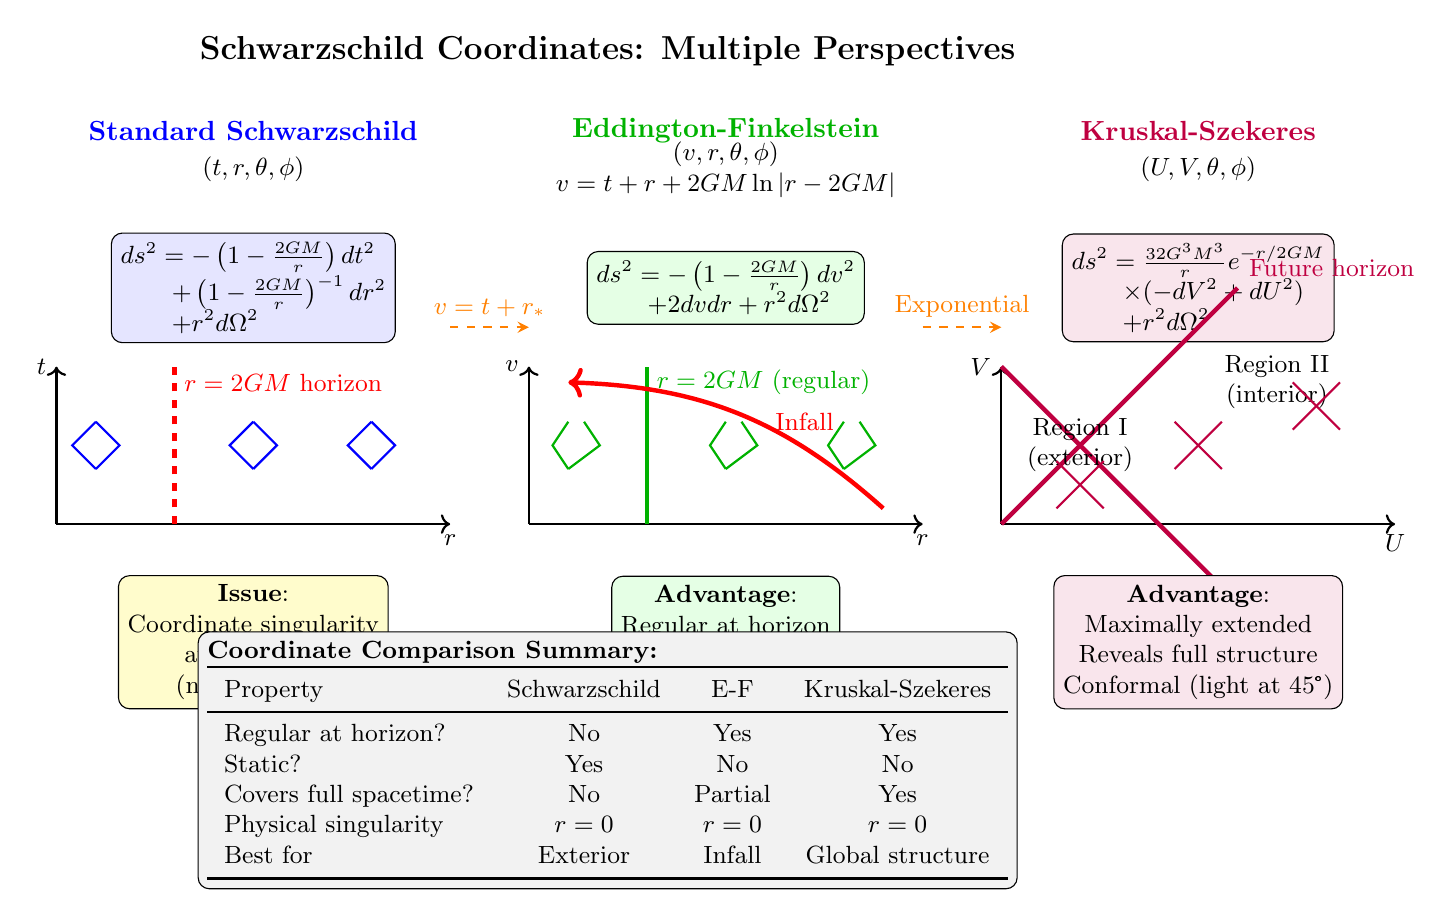
\begin{tikzpicture}[scale=1.0, every node/.style={font=\small}]

% Title
\node[font=\bfseries\large] at (7, 5.5) {Schwarzschild Coordinates: Multiple Perspectives};

% Left panel: Standard Schwarzschild (t, r, theta, phi)
\begin{scope}[shift={(0,0)}]
    \node[font=\bfseries, blue] at (2.5, 4.5) {Standard Schwarzschild};
    \node[align=center] at (2.5, 4) {$(t, r, \theta, \phi)$};
    
    % Metric
    \node[draw, fill=blue!10, align=left, rounded corners] at (2.5, 2.5) {
        $ds^2 = -\left(1-\frac{2GM}{r}\right)dt^2$\\
        \qquad $+ \left(1-\frac{2GM}{r}\right)^{-1}dr^2$\\
        \qquad $+ r^2 d\Omega^2$
    };
    
    % Spacetime diagram
    \draw[thick, ->] (0, -0.5) -- (0, 1.5) node[left] {$t$};
    \draw[thick, ->] (0, -0.5) -- (5, -0.5) node[below] {$r$};
    
    % Event horizon
    \draw[red, ultra thick, dashed] (1.5, -0.5) -- (1.5, 1.5);
    \node[red, right] at (1.5, 1.3) {$r=2GM$ horizon};
    
    % Light cones
    \foreach \x in {0.5, 2.5, 4} {
        \draw[blue, thick] (\x, 0.2) -- (\x+0.3, 0.5) -- (\x, 0.8);
        \draw[blue, thick] (\x, 0.2) -- (\x-0.3, 0.5) -- (\x, 0.8);
    }
    
    % Issue annotation
    \node[draw, fill=yellow!20, align=center, rounded corners] at (2.5, -2) {
        \textbf{Issue}:\\
        Coordinate singularity\\
        at $r=2GM$\\
        (not physical)
    };
\end{scope}

% Middle panel: Eddington-Finkelstein (v, r, theta, phi)
\begin{scope}[shift={(6,0)}]
    \node[font=\bfseries, green!70!black] at (2.5, 4.5) {Eddington-Finkelstein};
    \node[align=center] at (2.5, 4) {$(v, r, \theta, \phi)$\\$v = t + r + 2GM\ln|r-2GM|$};
    
    % Metric
    \node[draw, fill=green!10, align=left, rounded corners] at (2.5, 2.5) {
        $ds^2 = -\left(1-\frac{2GM}{r}\right)dv^2$\\
        \qquad $+ 2dvdr + r^2 d\Omega^2$
    };
    
    % Spacetime diagram
    \draw[thick, ->] (0, -0.5) -- (0, 1.5) node[left] {$v$};
    \draw[thick, ->] (0, -0.5) -- (5, -0.5) node[below] {$r$};
    
    % Event horizon (regular now)
    \draw[green!70!black, ultra thick] (1.5, -0.5) -- (1.5, 1.5);
    \node[green!70!black, right] at (1.5, 1.3) {$r=2GM$ (regular)};
    
    % Light cones (tilted inward)
    \foreach \x in {0.5, 2.5, 4} {
        \draw[green!70!black, thick] (\x, 0.2) -- (\x+0.4, 0.5) -- (\x+0.2, 0.8);
        \draw[green!70!black, thick] (\x, 0.2) -- (\x-0.2, 0.5) -- (\x, 0.8);
    }
    
    % Infalling path
    \draw[red, ultra thick, ->] (4.5, -0.3) to[bend right=20] (0.5, 1.3);
    \node[red] at (3.5, 0.8) {Infall};
    
    % Advantage annotation
    \node[draw, fill=green!10, align=center, rounded corners] at (2.5, -2) {
        \textbf{Advantage}:\\
        Regular at horizon\\
        Infalling observer\\
        perspective
    };
\end{scope}

% Right panel: Kruskal-Szekeres (U, V, theta, phi)
\begin{scope}[shift={(12,0)}]
    \node[font=\bfseries, purple] at (2.5, 4.5) {Kruskal-Szekeres};
    \node[align=center] at (2.5, 4) {$(U, V, \theta, \phi)$};
    
    % Metric
    \node[draw, fill=purple!10, align=left, rounded corners] at (2.5, 2.5) {
        $ds^2 = \frac{32G^3M^3}{r}e^{-r/2GM}$\\
        \qquad $\times (-dV^2 + dU^2)$\\
        \qquad $+ r^2 d\Omega^2$
    };
    
    % Spacetime diagram (conformal)
    \draw[thick, ->] (0, -0.5) -- (0, 1.5) node[left] {$V$};
    \draw[thick, ->] (0, -0.5) -- (5, -0.5) node[below] {$U$};
    
    % Horizons (45 degree lines)
    \draw[purple, ultra thick] (0, -0.5) -- (3, 2.5) node[above right] {Future horizon};
    \draw[purple, ultra thick] (0, 1.5) -- (3, -1.5);
    
    % Regions
    \node[align=center] at (1, 0.5) {Region I\\(exterior)};
    \node[align=center] at (3.5, 1.3) {Region II\\(interior)};
    
    % Light cones (45 degrees everywhere)
    \foreach \x/\y in {1/0, 2.5/0.5, 4/1} {
        \draw[purple, thick] (\x, \y) -- (\x+0.3, \y+0.3);
        \draw[purple, thick] (\x, \y) -- (\x-0.3, \y+0.3);
        \draw[purple, thick] (\x, \y) -- (\x+0.3, \y-0.3);
        \draw[purple, thick] (\x, \y) -- (\x-0.3, \y-0.3);
    }
    
    % Advantage annotation
    \node[draw, fill=purple!10, align=center, rounded corners] at (2.5, -2) {
        \textbf{Advantage}:\\
        Maximally extended\\
        Reveals full structure\\
        Conformal (light at 45°)
    };
\end{scope}

% Comparison table at bottom
\node[draw, fill=gray!10, align=left, rounded corners] at (7, -3.5) {
    \textbf{Coordinate Comparison Summary:}\\
    \begin{tabular}{lccc}
    \toprule
    Property & Schwarzschild & E-F & Kruskal-Szekeres \\
    \midrule
    Regular at horizon? & No & Yes & Yes \\
    Static? & Yes & No & No \\
    Covers full spacetime? & No & Partial & Yes \\
    Physical singularity & $r=0$ & $r=0$ & $r=0$ \\
    Best for & Exterior & Infall & Global structure \\
    \bottomrule
    \end{tabular}
};

% Transformation arrows
\draw[->, >=stealth, thick, dashed, orange] (5, 2) -- (6, 2) node[midway, above] {$v=t+r_*$};
\draw[->, >=stealth, thick, dashed, orange] (11, 2) -- (12, 2) node[midway, above] {Exponential};

\end{tikzpicture}
\caption{Three coordinate systems for Schwarzschild spacetime. Standard Schwarzschild coordinates have coordinate singularity at event horizon. Eddington-Finkelstein coordinates regular at horizon, good for infalling observers. Kruskal-Szekeres coordinates maximally extended, reveal complete spacetime structure including black/white hole regions. All describe same physical geometry; coordinate choice determines what features are manifest. Table compares key properties.}
\label{fig:schwarzschild_coordinates}
\end{figure}

\caption{Three coordinate systems for Schwarzschild spacetime: Standard (singular at horizon), Eddington-Finkelstein (regular at horizon, good for infalling observers), Kruskal-Szekeres (maximally extended, reveals global structure). \mphys{Same physical geometry, different coordinate choices---horizon singularity is coordinate artifact, not physical.}}
\label{fig:prelim:schwarzschild-coords}
\end{figure}

\mcaution{Coordinate singularity at $r = 2GM$ in standard Schwarzschild coordinates is artifact of coordinate choice. Physical singularity at $r = 0$ (curvature invariants diverge) is real.}

\subsubsection{Tensor Comparison Matrices}

% Additional Comparison Matrices
% File: tab_tensor_comparison_matrices.tex
% Purpose: Multi-dimensional comparison matrices for tensor properties
% For: Chapter 1 - Mathematical Preliminaries

\begin{table}[htbp]
\centering
\caption{Comparison matrix: Tensor transformation properties under coordinate changes $x^\mu \to x'^{\mu}$.}
\label{tab:tensor_transformations}
\small
\begin{tabular}{lcccl}
\toprule
\textbf{Object} & \textbf{Type} & \textbf{Transform as} & \textbf{Indices} & \textbf{Example} \\
\midrule
Scalar & $(0,0)$ & $\phi'(x') = \phi(x)$ & None & Temperature $T$ \\
Vector & $(1,0)$ & $V'^{\mu} = \frac{\partial x'^{\mu}}{\partial x^\nu} V^\nu$ & Upper & Velocity $u^\mu$ \\
Covector & $(0,1)$ & $\omega'_\mu = \frac{\partial x^\nu}{\partial x'^{\mu}} \omega_\nu$ & Lower & Gradient $\partial_\mu \phi$ \\
Metric & $(0,2)$ & $g'_{\mu\nu} = \frac{\partial x^\alpha}{\partial x'^{\mu}} \frac{\partial x^\beta}{\partial x'^{\nu}} g_{\alpha\beta}$ & Lower-lower & $g_{\mu\nu}$ \\
\midrule
Christoffel & Not tensor & Has inhomogeneous term & Mixed & $\Gamma^\mu_{\alpha\beta}$ \\
Riemann & $(1,3)$ & Tensor law & 1 up, 3 down & $R^\alpha_{\beta\mu\nu}$ \\
Ricci & $(0,2)$ & Tensor law & Lower-lower & $R_{\mu\nu}$ \\
Einstein & $(0,2)$ & Tensor law & Lower-lower & $G_{\mu\nu}$ \\
\bottomrule
\end{tabular}
\end{table}

\begin{table}[htbp]
\centering
\caption{Comparison matrix: Index manipulation operations and their physical/geometric meanings.}
\label{tab:index_operations}
\small
\begin{tabular}{llcp{5cm}}
\toprule
\textbf{Operation} & \textbf{Notation} & \textbf{Formula} & \textbf{Physical/Geometric Meaning} \\
\midrule
\textbf{Raising} & $V_\mu \to V^\mu$ & $V^\mu = g^{\mu\nu} V_\nu$ & Convert covector to vector using metric \\
\textbf{Lowering} & $V^\mu \to V_\mu$ & $V_\mu = g_{\mu\nu} V^\nu$ & Convert vector to covector using metric \\
\textbf{Contraction} & $(m,n) \to (m-1,n-1)$ & $T^\mu_{\ \ \mu} = \sum_\mu T^\mu_{\ \ \mu}$ & Sum over repeated index (trace) \\
\textbf{Symmetrization} & $T_{(\mu\nu)}$ & $\frac{1}{2}(T_{\mu\nu} + T_{\nu\mu})$ & Extract symmetric part \\
\textbf{Antisymmetrization} & $T_{[\mu\nu]}$ & $\frac{1}{2}(T_{\mu\nu} - T_{\nu\mu})$ & Extract antisymmetric part (2-form) \\
\textbf{Covariant deriv.} & $\nabla_\mu V^\nu$ & $\partial_\mu V^\nu + \Gamma^\nu_{\mu\alpha} V^\alpha$ & Parallel transport-compatible derivative \\
\textbf{Lie derivative} & $\mathcal{L}_X Y$ & $[X,Y]$ (commutator) & Directional change along flow \\
\midrule
\multicolumn{4}{l}{\textit{\textbf{Algebraic Properties}}} \\
\textbf{Metric compatibility} & $\nabla_\alpha g_{\mu\nu} = 0$ & -- & Covariant derivative commutes with raising/lowering \\
\textbf{Torsion-free} & $\Gamma^\mu_{\alpha\beta} = \Gamma^\mu_{\beta\alpha}$ & -- & Connection symmetric in lower indices \\
\textbf{Bianchi identity} & $\nabla_{[\alpha} R_{\beta\gamma]\delta\epsilon} = 0$ & -- & Integrability condition for curvature \\
\bottomrule
\end{tabular}
\end{table}

\begin{table}[htbp]
\centering
\caption{Cross-comparison matrix: Geometric objects across different geometric structures.}
\label{tab:geometry_comparison}
\footnotesize
\begin{tabular}{lp{2.8cm}p{2.8cm}p{2.8cm}p{2.8cm}}
\toprule
\textbf{Object} & \textbf{Euclidean ($\mathbb{E}^n$)} & \textbf{Riemannian ($M,g$)} & \textbf{Pseudo-Riemannian ($M,g$)} & \textbf{Symplectic ($M,\omega$)} \\
\midrule
\textbf{Metric} & $\delta_{ij}$ (flat, positive) & $g_{ij} > 0$ (positive-definite) & $g_{\mu\nu}$ (indefinite, signature) & No metric (only 2-form $\omega$) \\
\textbf{Connection} & $\Gamma = 0$ (flat) & Levi-Civita (metric-compatible) & Levi-Civita (metric-compatible) & Various (not unique) \\
\textbf{Curvature} & $R = 0$ everywhere & $R_{ijkl}$ (intrinsic) & $R_{\mu\nu\alpha\beta}$ (intrinsic) & Not fundamental \\
\textbf{Parallel transport} & Path-independent & Path-dependent if $R \neq 0$ & Path-dependent if $R \neq 0$ & Not standard \\
\textbf{Geodesics} & Straight lines & Curves extremizing length & Curves extremizing interval (timelike/null/spacelike) & Hamiltonian flow \\
\midrule
\textbf{Physical application} & Classical mechanics (flat space) & Elasticity, surfaces & General relativity (spacetime) & Phase space, Hamiltonian mechanics \\
\textbf{Signature} & $(+,+,\ldots,+)$ & $(+,+,\ldots,+)$ & $(-,+,+,+)$ (or reverse) & $N/A$ \\
\textbf{Volume element} & $dV = dx^1 \cdots dx^n$ & $dV = \sqrt{g} dx^1 \cdots dx^n$ & $dV = \sqrt{-g} dx^0 \cdots dx^{n-1}$ & $\omega^n / n!$ \\
\textbf{Chapter 1 focus} & Starting point & Generalization & Central topic (GR) & Mentioned (QM phase space) \\
\bottomrule
\end{tabular}
\end{table}

\begin{table}[htbp]
\centering
\caption{Symmetry comparison matrix: Types of spacetime symmetries and their consequences (Noether theorem).}
\label{tab:symmetry_matrix}
\small
\begin{tabular}{llp{4cm}l}
\toprule
\textbf{Symmetry} & \textbf{Killing vector} & \textbf{Physical interpretation} & \textbf{Conserved quantity} \\
\midrule
\textbf{Time translation} & $\xi^\mu = (1, 0, 0, 0)$ & Static spacetime, $\partial_t g_{\mu\nu} = 0$ & Energy $E$ \\
\textbf{Spatial translation} & $\xi^\mu = (0, \vec{n})$ & Homogeneous space & Linear momentum $\vec{p}$ \\
\textbf{Rotation} & $\xi^\mu = (0, \vec{r} \times \vec{n})$ & Spherical symmetry (part) & Angular momentum $\vec{L}$ \\
\textbf{Boost} & $\xi^\mu = (x^i, t \delta^i_j)$ & Lorentz invariance & Center of mass motion \\
\midrule
\multicolumn{4}{l}{\textit{\textbf{Special Cases}}} \\
Minkowski & 10 Killing vectors & Poincaré symmetry (ISO(1,3)) & Energy-momentum tensor conserved \\
Schwarzschild & 4 Killing vectors & $\partial_t, \partial_\phi$ + 2 spatial rotations & Energy, angular momentum \\
FLRW & 6 Killing vectors & Spatial isotropy + homogeneity & Reduces Einstein eqs. to Friedmann \\
Kerr & 2 Killing vectors & Axisymmetry + stationarity & Energy, angular momentum \\
pp-waves & 5 Killing vectors & Plane wave symmetry & Simplifies geodesics \\
\midrule
\textbf{No symmetries} & Generic & Most spacetimes & No conserved quantities (generally) \\
\bottomrule
\end{tabular}
\end{table}


\mxref{Killing vectors and conserved quantities: Schwarzschild (4), FLRW (6), Minkowski (10). See \S\ref{sec:symmetries-conservation} for detailed treatment.}

\subsubsection{GR to Quantum Gravity Connection}

\begin{figure}[htbp]
\centering
% GR to QFT Connection Diagram
% File: tikz_gr_to_qft.tex
% Purpose: Visualize mathematical path from general relativity to quantum field theory
% For: Chapter 1 - Mathematical Preliminaries

\begin{figure}[htbp]
\centering
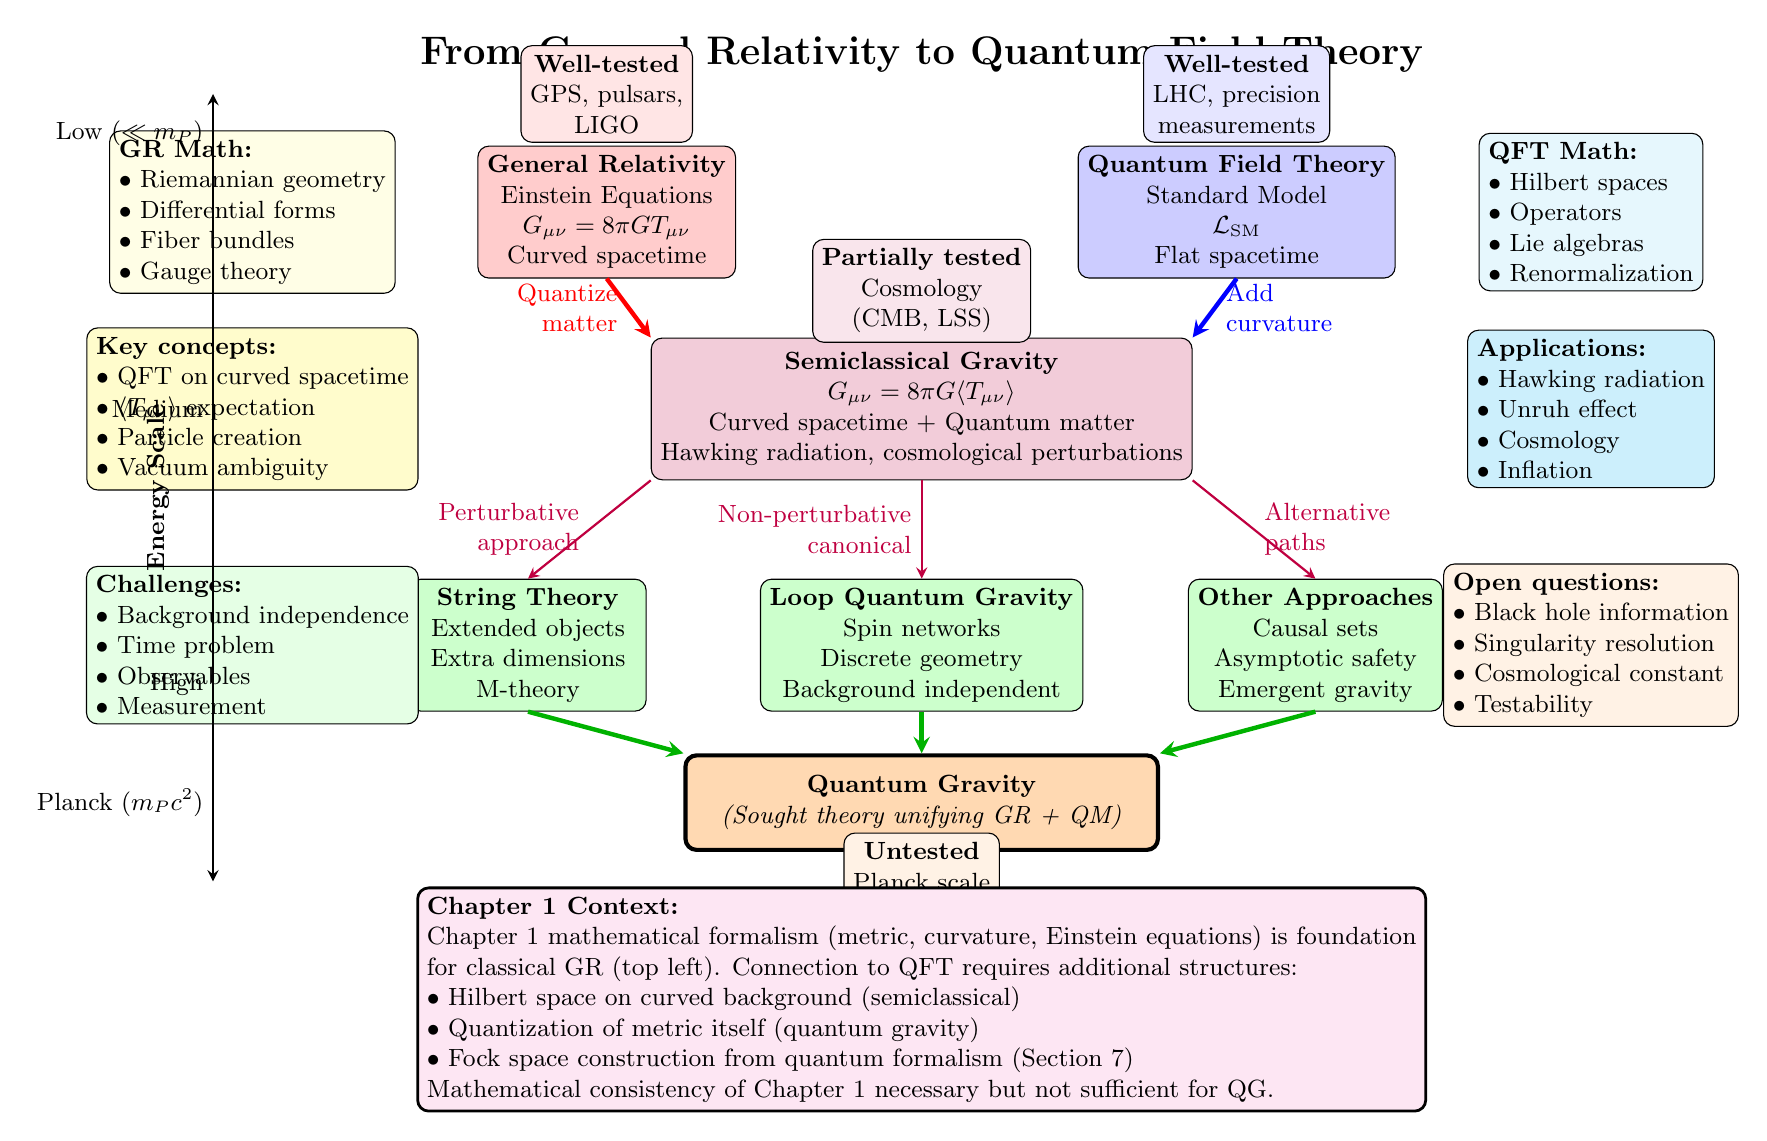
\begin{tikzpicture}[scale=1.0, every node/.style={font=\small}]

% Title
\node[font=\bfseries\Large] at (7, 9) {From General Relativity to Quantum Field Theory};

% Top: Classical GR
\node[draw, fill=red!20, rounded corners, align=center, minimum width=3cm, minimum height=1.5cm] (gr) at (3, 7) {
    \textbf{General Relativity}\\
    Einstein Equations\\
    $G_{\mu\nu} = 8\pi G T_{\mu\nu}$\\
    Curved spacetime
};

% Classical QFT (separate)
\node[draw, fill=blue!20, rounded corners, align=center, minimum width=3cm, minimum height=1.5cm] (qft) at (11, 7) {
    \textbf{Quantum Field Theory}\\
    Standard Model\\
    $\mathcal{L}_{\text{SM}}$\\
    Flat spacetime
};

% Middle level: Semiclassical
\node[draw, fill=purple!20, rounded corners, align=center, minimum width=6cm, minimum height=1.8cm] (semiclassical) at (7, 4.5) {
    \textbf{Semiclassical Gravity}\\
    $G_{\mu\nu} = 8\pi G \langle T_{\mu\nu} \rangle$\\
    Curved spacetime + Quantum matter\\
    Hawking radiation, cosmological perturbations
};

% Lower level: Approaches to quantum gravity
\node[draw, fill=green!20, rounded corners, align=center, minimum width=3cm, minimum height=1.5cm] (strings) at (2, 1.5) {
    \textbf{String Theory}\\
    Extended objects\\
    Extra dimensions\\
    M-theory
};

\node[draw, fill=green!20, rounded corners, align=center, minimum width=3cm, minimum height=1.5cm] (lqg) at (7, 1.5) {
    \textbf{Loop Quantum Gravity}\\
    Spin networks\\
    Discrete geometry\\
    Background independent
};

\node[draw, fill=green!20, rounded corners, align=center, minimum width=3cm, minimum height=1.5cm] (other) at (12, 1.5) {
    \textbf{Other Approaches}\\
    Causal sets\\
    Asymptotic safety\\
    Emergent gravity
};

% Bottom: Unified theory
\node[draw, fill=orange!30, rounded corners, align=center, minimum width=6cm, minimum height=1.2cm, line width=1.5pt] (qg) at (7, -0.5) {
    \textbf{Quantum Gravity}\\
    \emph{(Sought theory unifying GR + QM)}
};

% Arrows: Classical to semiclassical
\draw[->, >=stealth, ultra thick, red] (gr.south) -- (semiclassical.north west) node[midway, left, align=right] {Quantize\\matter};
\draw[->, >=stealth, ultra thick, blue] (qft.south) -- (semiclassical.north east) node[midway, right, align=left] {Add\\curvature};

% Arrows: Semiclassical to approaches
\draw[->, >=stealth, thick, purple] (semiclassical.south west) -- (strings.north) node[midway, left, align=right] {Perturbative\\approach};
\draw[->, >=stealth, thick, purple] (semiclassical.south) -- (lqg.north) node[midway, left, align=right] {Non-perturbative\\canonical};
\draw[->, >=stealth, thick, purple] (semiclassical.south east) -- (other.north) node[midway, right, align=left] {Alternative\\paths};

% Arrows: Approaches to quantum gravity
\draw[->, >=stealth, ultra thick, green!70!black] (strings.south) -- (qg.north west);
\draw[->, >=stealth, ultra thick, green!70!black] (lqg.south) -- (qg.north);
\draw[->, >=stealth, ultra thick, green!70!black] (other.south) -- (qg.north east);

% Key mathematical structures (side annotations)
\node[draw, fill=yellow!10, align=left, rounded corners] at (-1.5, 7) {
    \textbf{GR Math:}\\
    $\bullet$ Riemannian geometry\\
    $\bullet$ Differential forms\\
    $\bullet$ Fiber bundles\\
    $\bullet$ Gauge theory
};

\node[draw, fill=cyan!10, align=left, rounded corners] at (15.5, 7) {
    \textbf{QFT Math:}\\
    $\bullet$ Hilbert spaces\\
    $\bullet$ Operators\\
    $\bullet$ Lie algebras\\
    $\bullet$ Renormalization
};

\node[draw, fill=yellow!20, align=left, rounded corners] at (-1.5, 4.5) {
    \textbf{Key concepts:}\\
    $\bullet$ QFT on curved spacetime\\
    $\bullet$ $\langle T_{\mu\nu} \rangle$ expectation\\
    $\bullet$ Particle creation\\
    $\bullet$ Vacuum ambiguity
};

\node[draw, fill=cyan!20, align=left, rounded corners] at (15.5, 4.5) {
    \textbf{Applications:}\\
    $\bullet$ Hawking radiation\\
    $\bullet$ Unruh effect\\
    $\bullet$ Cosmology\\
    $\bullet$ Inflation
};

\node[draw, fill=green!10, align=left, rounded corners] at (-1.5, 1.5) {
    \textbf{Challenges:}\\
    $\bullet$ Background independence\\
    $\bullet$ Time problem\\
    $\bullet$ Observables\\
    $\bullet$ Measurement
};

\node[draw, fill=orange!10, align=left, rounded corners] at (15.5, 1.5) {
    \textbf{Open questions:}\\
    $\bullet$ Black hole information\\
    $\bullet$ Singularity resolution\\
    $\bullet$ Cosmological constant\\
    $\bullet$ Testability
};

% Energy scales
\draw[<->, >=stealth, thick] (-2, -1.5) -- (-2, 8.5);
\node[rotate=90] at (-2.7, 3.5) {\textbf{Energy Scale}};

\node[left] at (-2, 8) {Low ($\ll m_P$)};
\node[left] at (-2, 4.5) {Medium};
\node[left] at (-2, 1) {High};
\node[left] at (-2, -0.5) {Planck ($m_P c^2$)};

% Experimental status
\node[draw, fill=red!10, align=center, rounded corners] at (3, 8.5) {
    \textbf{Well-tested}\\
    GPS, pulsars,\\
    LIGO
};

\node[draw, fill=blue!10, align=center, rounded corners] at (11, 8.5) {
    \textbf{Well-tested}\\
    LHC, precision\\
    measurements
};

\node[draw, fill=purple!10, align=center, rounded corners] at (7, 6) {
    \textbf{Partially tested}\\
    Cosmology\\
    (CMB, LSS)
};

\node[draw, fill=orange!10, align=center, rounded corners] at (7, -1.5) {
    \textbf{Untested}\\
    Planck scale\\
    $\sim 10^{19}$ GeV
};

% Chapter 1 context box
\node[draw, fill=magenta!10, align=left, rounded corners, line width=1pt] at (7, -3) {
    \textbf{Chapter 1 Context:}\\
    Chapter 1 mathematical formalism (metric, curvature, Einstein equations) is foundation\\
    for classical GR (top left). Connection to QFT requires additional structures:\\
    $\bullet$ Hilbert space on curved background (semiclassical)\\
    $\bullet$ Quantization of metric itself (quantum gravity)\\
    $\bullet$ Fock space construction from quantum formalism (Section 7)\\
    Mathematical consistency of Chapter 1 necessary but not sufficient for QG.
};

\end{tikzpicture}
\caption{Mathematical and conceptual pathway from classical general relativity (top left) and quantum field theory on flat spacetime (top right) through semiclassical gravity (middle) to sought quantum gravity theory (bottom). Energy scales on left, experimental status indicated. Chapter 1 formalism provides classical GR foundation; additional mathematical structures needed for quantum regime. Multiple approaches to quantum gravity shown (string theory, loop quantum gravity, alternatives) with current status. Key challenges and open questions annotated.}
\label{fig:gr_to_qft}
\end{figure}

\caption{Mathematical pathway from classical GR to quantum gravity: GR (deterministic curved spacetime) + QFT (quantum matter fields) $\to$ semiclassical gravity ($G_{\mu\nu} = 8\pi G \langle T_{\mu\nu} \rangle$) $\to$ full quantum gravity approaches (string theory, loop quantum gravity, etc.). \mphys{Planck scale ($\ell_P = 10^{-35}$ m) is where quantum gravity becomes essential.}}
\label{fig:prelim:gr-to-qft}
\end{figure}

\textbf{Open challenges}: Background independence, time problem, observables in quantum gravity, cosmological constant problem, black hole information paradox.

\subsubsection{Tidal Forces and Geodesic Deviation}

\begin{figure}[htbp]
\centering
% Tidal Forces and Geodesic Deviation
% File: tikz_tidal_forces.tex
% Purpose: Visualize geodesic deviation equation and tidal effects
% For: Chapter 1 - Mathematical Preliminaries

\begin{figure}[htbp]
\centering
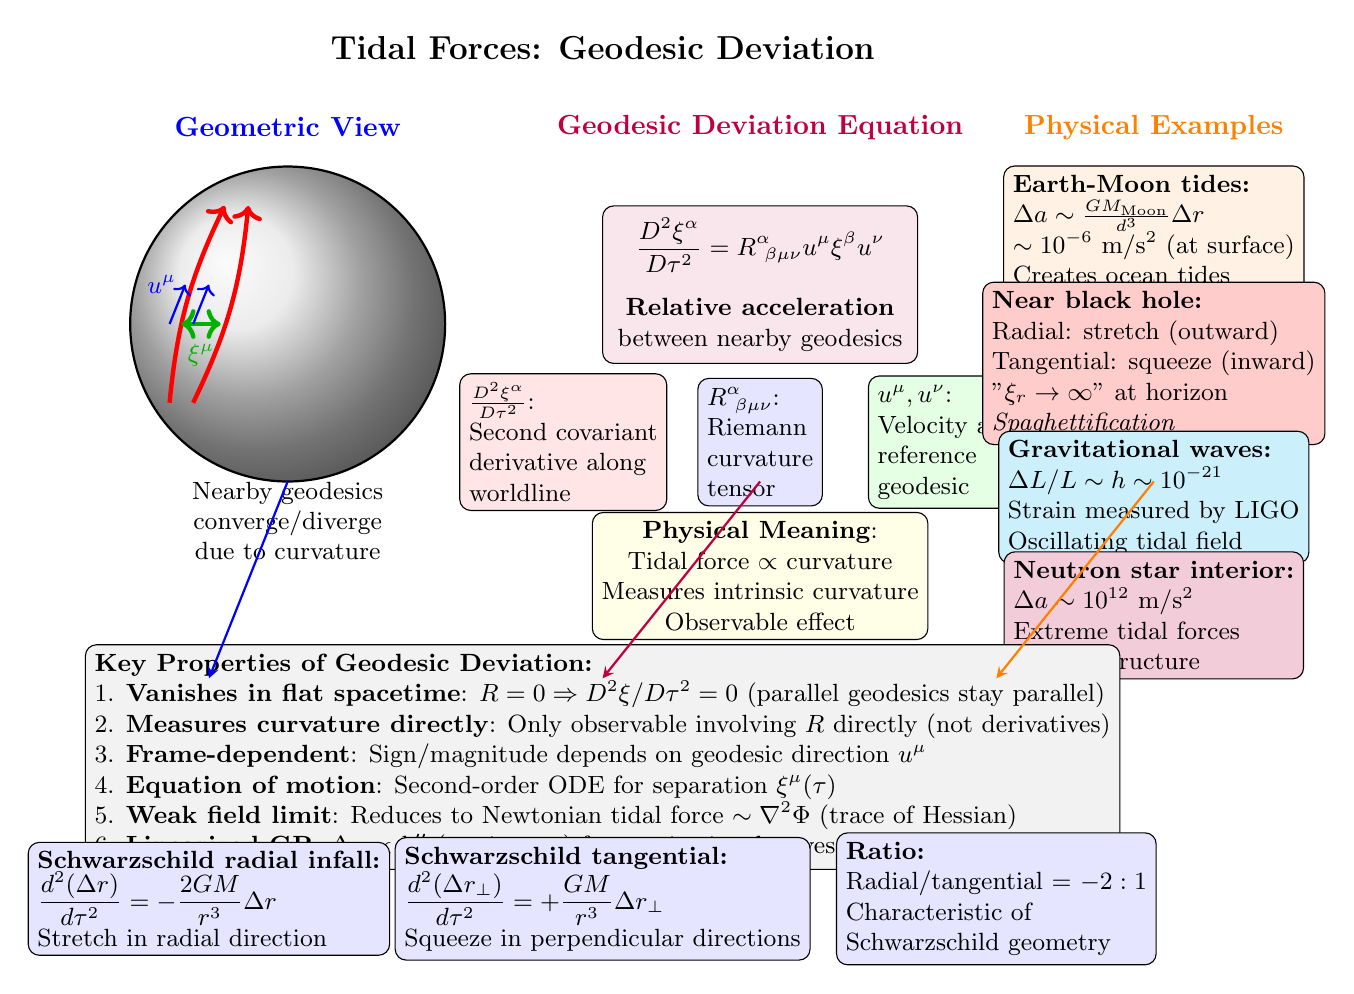
\begin{tikzpicture}[scale=1.0, every node/.style={font=\small}]

% Title
\node[font=\bfseries\large] at (7, 7.5) {Tidal Forces: Geodesic Deviation};

% Left panel: Geometric picture
\begin{scope}[shift={(0,0)}]
    \node[font=\bfseries, blue] at (3, 6.5) {Geometric View};
    
    % Curved surface (sphere segment)
    \shade[ball color=gray!20] (3, 4) circle (2cm);
    \draw[thick] (3, 4) circle (2cm);
    
    % Two nearby geodesics
    \draw[red, ultra thick, ->] (1.5, 3) to[bend left=10] (2.2, 5.5);
    \draw[red, ultra thick, ->] (1.8, 3) to[bend right=10] (2.5, 5.5);
    
    % Separation vector
    \draw[green!70!black, ultra thick, <->] (1.65, 4) -- (2.15, 4);
    \node[green!70!black] at (1.9, 3.6) {$\xi^\mu$};
    
    % Tangent vectors
    \draw[blue, thick, ->] (1.5, 4) -- (1.7, 4.5);
    \draw[blue, thick, ->] (1.8, 4) -- (2.0, 4.5);
    \node[blue] at (1.4, 4.5) {$u^\mu$};
    
    % Curvature annotation
    \node[align=center] at (3, 1.5) {
        Nearby geodesics\\
        converge/diverge\\
        due to curvature
    };
\end{scope}

% Center panel: Equation
\begin{scope}[shift={(6,0)}]
    \node[font=\bfseries, purple] at (3, 6.5) {Geodesic Deviation Equation};
    
    % Main equation box
    \node[draw, fill=purple!10, align=center, rounded corners, minimum width=4cm, minimum height=2cm] at (3, 4.5) {
        $\displaystyle \frac{D^2 \xi^\alpha}{D\tau^2} = R^\alpha_{\ \beta\mu\nu} u^\mu \xi^\beta u^\nu$\\[0.3cm]
        \textbf{Relative acceleration}\\
        between nearby geodesics
    };
    
    % Component breakdown
    \node[draw, fill=red!10, align=left, rounded corners] at (0.5, 2.5) {
        $\frac{D^2 \xi^\alpha}{D\tau^2}$:\\
        Second covariant\\
        derivative along\\
        worldline
    };
    
    \node[draw, fill=blue!10, align=left, rounded corners] at (3, 2.5) {
        $R^\alpha_{\ \beta\mu\nu}$:\\
        Riemann\\
        curvature\\
        tensor
    };
    
    \node[draw, fill=green!10, align=left, rounded corners] at (5.5, 2.5) {
        $u^\mu, u^\nu$:\\
        Velocity along\\
        reference\\
        geodesic
    };
    
    % Physical meaning
    \node[draw, fill=yellow!10, align=center, rounded corners] at (3, 0.8) {
        \textbf{Physical Meaning}:\\
        Tidal force $\propto$ curvature\\
        Measures intrinsic curvature\\
        Observable effect
    };
\end{scope}

% Right panel: Tidal examples
\begin{scope}[shift={(11,0)}]
    \node[font=\bfseries, orange] at (3, 6.5) {Physical Examples};
    
    % Earth-Moon system
    \node[draw, fill=orange!10, align=left, rounded corners] at (3, 5.2) {
        \textbf{Earth-Moon tides:}\\
        $\Delta a \sim \frac{GM_{\text{Moon}}}{d^3} \Delta r$\\
        $\sim 10^{-6}$ m/s$^2$ (at surface)\\
        Creates ocean tides
    };
    
    % Spaghettification
    \node[draw, fill=red!20, align=left, rounded corners] at (3, 3.5) {
        \textbf{Near black hole:}\\
        Radial: stretch (outward)\\
        Tangential: squeeze (inward)\\
        "$\xi_r \to \infty$" at horizon\\
        \emph{Spaghettification}
    };
    
    % LIGO
    \node[draw, fill=cyan!20, align=left, rounded corners] at (3, 1.8) {
        \textbf{Gravitational waves:}\\
        $\Delta L / L \sim h \sim 10^{-21}$\\
        Strain measured by LIGO\\
        Oscillating tidal field
    };
    
    % Neutron star
    \node[draw, fill=purple!20, align=left, rounded corners] at (3, 0.3) {
        \textbf{Neutron star interior:}\\
        $\Delta a \sim 10^{12}$ m/s$^2$\\
        Extreme tidal forces\\
        Affects structure
    };
\end{scope}

% Bottom: Mathematical details
\node[draw, fill=gray!10, align=left, rounded corners] at (7, -1.5) {
    \textbf{Key Properties of Geodesic Deviation:}\\
    1. \textbf{Vanishes in flat spacetime}: $R = 0 \Rightarrow D^2\xi/D\tau^2 = 0$ (parallel geodesics stay parallel)\\
    2. \textbf{Measures curvature directly}: Only observable involving $R$ directly (not derivatives)\\
    3. \textbf{Frame-dependent}: Sign/magnitude depends on geodesic direction $u^\mu$\\
    4. \textbf{Equation of motion}: Second-order ODE for separation $\xi^\mu(\tau)$\\
    5. \textbf{Weak field limit}: Reduces to Newtonian tidal force $\sim \nabla^2 \Phi$ (trace of Hessian)\\
    6. \textbf{Linearized GR}: $\Delta a \propto h''$ (strain rate) for gravitational waves
};

% Schwarzschild specific formula
\node[draw, fill=blue!10, align=left, rounded corners] at (2, -3.3) {
    \textbf{Schwarzschild radial infall:}\\
    $\displaystyle \frac{d^2(\Delta r)}{d\tau^2} = -\frac{2GM}{r^3} \Delta r$\\
    Stretch in radial direction
};

\node[draw, fill=blue!10, align=left, rounded corners] at (7, -3.3) {
    \textbf{Schwarzschild tangential:}\\
    $\displaystyle \frac{d^2(\Delta r_\perp)}{d\tau^2} = +\frac{GM}{r^3} \Delta r_\perp$\\
    Squeeze in perpendicular directions
};

\node[draw, fill=blue!10, align=left, rounded corners] at (12, -3.3) {
    \textbf{Ratio:}\\
    Radial/tangential = $-2:1$\\
    Characteristic of\\
    Schwarzschild geometry
};

% Connecting lines
\draw[->, >=stealth, thick, blue] (3, 2) -- (2, -0.5);
\draw[->, >=stealth, thick, purple] (9, 2) -- (7, -0.5);
\draw[->, >=stealth, thick, orange] (14, 2) -- (12, -0.5);

\end{tikzpicture}
\caption{Tidal forces as manifestation of spacetime curvature through geodesic deviation equation. Left: Geometric picture showing two nearby geodesics with separation vector $\xi^\mu$ that accelerates relative to reference geodesic with velocity $u^\mu$. Center: Geodesic deviation equation $D^2\xi^\alpha/D\tau^2 = R^\alpha_{\ \beta\mu\nu} u^\mu \xi^\beta u^\nu$ relating relative acceleration to Riemann curvature. Right: Physical examples from ocean tides ($10^{-6}$ m/s$^2$) to black hole spaghettification to LIGO strain measurements ($10^{-21}$) to neutron star interiors ($10^{12}$ m/s$^2$). Bottom: Mathematical properties and Schwarzschild-specific formulas showing characteristic 2:1 stretch-squeeze ratio. Geodesic deviation provides direct observable measurement of curvature.}
\label{fig:tidal_forces}
\end{figure}

\caption{Geodesic deviation equation: $D^2 \xi^\alpha/D\tau^2 = R^\alpha{}_{\beta\mu\nu} u^\mu \xi^\beta u^\nu$. Two nearby geodesics separate due to curvature. Tidal acceleration spans 15 orders of magnitude: Earth-Moon tides ($\sim 10^{-6}$ m/s$^2$) to neutron star interiors ($\sim 10^{12}$ m/s$^2$). \mphys{Riemann tensor directly measures tidal forces---operational definition of spacetime curvature.}}
\label{fig:prelim:tidal-forces}
\end{figure}

\textbf{Schwarzschild tidal formulas}:
\begin{align}
  \frac{d^2(\Delta r)}{d\tau^2} &= -\frac{2GM}{r^3} \Delta r \quad \text{(radial stretch)} \\
  \frac{d^2(\Delta r_\perp)}{d\tau^2} &= +\frac{GM}{r^3} \Delta r_\perp \quad \text{(tangential squeeze)}
\end{align}

Characteristic 2:1 ratio: Radial stretching is twice tangential squeezing---signature of Schwarzschild geometry.

\subsubsection{Curvature Scales Catalog}

% Curvature Scales Comparison
% File: tab_curvature_scales.tex
% Purpose: Compare characteristic curvature scales across physical systems
% For: Chapter 1 - Mathematical Preliminaries

\begin{table}[htbp]
\centering
\caption{Curvature scales across physical systems: Ricci scalar $R$ and characteristic length scale $\ell_{\text{curv}} = |R|^{-1/2}$ (geometric units $c=G=1$).}
\label{tab:curvature_scales}
\small
\begin{tabular}{lcccp{4cm}}
\toprule
\textbf{Physical System} & \textbf{Ricci scalar $R$} & \textbf{Curv. length $\ell_{\text{curv}}$} & \textbf{$R/R_{\text{Planck}}$} & \textbf{Physical significance} \\
\midrule
\multicolumn{5}{l}{\textit{\textbf{Cosmological Scales}}} \\
Observable universe (present) & $\sim 10^{-52}$ m$^{-2}$ & $\sim 10^{26}$ m (Hubble) & $10^{-122}$ & Extremely weak curvature \\
Early universe ($t=1$ s) & $\sim 10^{-10}$ m$^{-2}$ & $\sim 10^{5}$ m & $10^{-80}$ & Post-BBN era \\
Inflation epoch & $\sim 10^{14}$ m$^{-2}$ & $\sim 10^{-7}$ m & $10^{-56}$ & Nearly exponential expansion \\
Planck epoch ($t=t_P$) & $\sim 10^{70}$ m$^{-2}$ & $\sim 10^{-35}$ m (Planck) & $1$ & Quantum gravity regime \\
\midrule
\multicolumn{5}{l}{\textit{\textbf{Astrophysical Objects}}} \\
Solar system (Earth orbit) & $\sim 10^{-27}$ m$^{-2}$ & $\sim 10^{13}$ m (0.1 AU) & $10^{-97}$ & Very weak field \\
Sun surface & $\sim 10^{-11}$ m$^{-2}$ & $\sim 10^{5}$ m & $10^{-81}$ & Newtonian limit valid \\
White dwarf & $\sim 10^{-6}$ m$^{-2}$ & $\sim 10^{3}$ m & $10^{-76}$ & Electron degeneracy pressure \\
Neutron star surface & $\sim 10^{8}$ m$^{-2}$ & $\sim 10^{-4}$ m (0.1 mm) & $10^{-62}$ & Strong field, post-Newtonian \\
Neutron star core & $\sim 10^{12}$ m$^{-2}$ & $\sim 10^{-6}$ m (1 μm) & $10^{-58}$ & Extreme curvature \\
\midrule
\multicolumn{5}{l}{\textit{\textbf{Black Holes}}} \\
Supermassive BH (M87*, $10^9 M_\odot$) & $\sim 10^{-24}$ m$^{-2}$ & $\sim 10^{12}$ m (2500 AU) & $10^{-94}$ & Weak curvature at horizon \\
Stellar BH ($10 M_\odot$) & $\sim 10^{-6}$ m$^{-2}$ & $\sim 10^{3}$ m (3 km) & $10^{-76}$ & Schwarzschild radius scale \\
Primordial BH ($M_\text{asteroid}$) & $\sim 10^{6}$ m$^{-2}$ & $\sim 10^{-3}$ m (1 mm) & $10^{-64}$ & Hawking radiation significant \\
Micro BH ($M_\text{Planck}$) & $\sim 10^{70}$ m$^{-2}$ & $\sim 10^{-35}$ m (Planck) & $1$ & Quantum regime \\
\midrule
\multicolumn{5}{l}{\textit{\textbf{Gravitational Waves (strain h, frequency f)}}} \\
LIGO detection (binary BH) & $\sim 10^{-42}$ strain & -- & -- & $h \sim 10^{-21}$, $f \sim 100$ Hz \\
Pulsar timing arrays & $\sim 10^{-30}$ strain & -- & -- & $h \sim 10^{-15}$, $f \sim 10^{-8}$ Hz \\
Cosmic GW background & $\sim 10^{-16}$ strain & -- & -- & Primordial, stochastic \\
\midrule
\multicolumn{5}{l}{\textit{\textbf{Comparison Scales}}} \\
Flat spacetime (Minkowski) & $R = 0$ exactly & $\ell_{\text{curv}} \to \infty$ & $0$ & Reference (no curvature) \\
Planck curvature & $R_P \sim 10^{70}$ m$^{-2}$ & $\ell_P \sim 10^{-35}$ m & $1$ & Quantum gravity threshold \\
Earth surface (2D) & $R_\oplus \sim 10^{-14}$ m$^{-2}$ & $R_\oplus \sim 6 \times 10^{6}$ m & -- & Spatial curvature only \\
\bottomrule
\end{tabular}
\end{table}

\begin{table}[htbp]
\centering
\caption{Regime classification for general relativity validity based on curvature scale and characteristic system parameters.}
\label{tab:gr_validity_regimes}
\small
\begin{tabular}{lp{3.5cm}p{3.5cm}p{4cm}}
\toprule
\textbf{Regime} & \textbf{Condition} & \textbf{Approximation} & \textbf{Examples} \\
\midrule
\textbf{Newtonian} & $\ell_{\text{curv}} \gg L_{\text{system}}$, $v \ll c$, $\Phi/c^2 \ll 1$ & $g_{00} \approx -(1+2\Phi/c^2)$, $g_{ij} \approx \delta_{ij}$ & Solar system, galaxies, most astrophysics \\
\midrule
\textbf{Post-Newtonian} & $\Phi/c^2 \sim 10^{-6}-10^{-2}$, $v/c \sim 0.1-0.3$ & Expansion in $v/c$ and $\Phi/c^2$ & Binary pulsars, GPS corrections, perihelion precession \\
\midrule
\textbf{Strong field} & $\Phi/c^2 \sim 0.1-0.5$, $v/c \sim 0.3-0.6$ & Full Einstein equations, numerical required & Neutron star mergers, close binaries, accretion disks \\
\midrule
\textbf{Extreme/relativistic} & $\ell_{\text{curv}} \sim L_{\text{system}}$, $v \to c$ & Numerical relativity, no approximations & Black hole horizons, GW emission during merger \\
\midrule
\textbf{Quantum gravity} & $\ell_{\text{curv}} \sim \ell_P$, $R \sim R_P$ & Classical GR breaks down, quantum effects dominant & Planck epoch, BH singularities (interior), micro black holes \\
\midrule
\textbf{Cosmological} & $\ell_{\text{curv}} \sim H_0^{-1}$, homogeneous & FLRW metric, Friedmann equations & CMB, large-scale structure, dark energy \\
\bottomrule
\end{tabular}
\end{table}

\begin{table}[htbp]
\centering
\caption{Dimensional analysis: Characteristic scales and their physical significance in general relativity.}
\label{tab:characteristic_scales}
\small
\begin{tabular}{lccl}
\toprule
\textbf{Scale} & \textbf{Value (SI)} & \textbf{Value (Natural)} & \textbf{Physical meaning} \\
\midrule
\multicolumn{4}{l}{\textit{\textbf{Fundamental Constants}}} \\
Speed of light $c$ & $3.0 \times 10^8$ m/s & $1$ & Spacetime conversion \\
Newton constant $G$ & $6.7 \times 10^{-11}$ m$^3$/kg/s$^2$ & $1$ & Gravitational coupling \\
Planck constant $\hbar$ & $1.1 \times 10^{-34}$ J$\cdot$s & $1$ & Quantum scale \\
\midrule
\multicolumn{4}{l}{\textit{\textbf{Derived Scales}}} \\
Planck length $\ell_P$ & $1.6 \times 10^{-35}$ m & $1$ & Quantum gravity length \\
Planck time $t_P$ & $5.4 \times 10^{-44}$ s & $1$ & Quantum gravity time \\
Planck mass $m_P$ & $2.2 \times 10^{-8}$ kg & $1$ & Quantum gravity mass \\
Planck energy $E_P$ & $1.2 \times 10^{19}$ GeV & $1$ & Quantum gravity energy \\
Planck density $\rho_P$ & $5.2 \times 10^{96}$ kg/m$^3$ & $1$ & Quantum gravity density \\
Planck curvature $R_P$ & $\ell_P^{-2} \sim 10^{70}$ m$^{-2}$ & $1$ & Quantum gravity curvature \\
\midrule
\multicolumn{4}{l}{\textit{\textbf{Astrophysical Scales}}} \\
Schwarzschild radius $r_s$ & $2GM/c^2$ & $2M$ & Black hole horizon \\
Solar mass $M_\odot$ & $2.0 \times 10^{30}$ kg & $1.5$ km & Gravitational radius unit \\
Hubble parameter $H_0$ & $2.2 \times 10^{-18}$ s$^{-1}$ & $10^{-61} \ell_P^{-1}$ & Cosmic expansion rate \\
Hubble length $H_0^{-1}$ & $1.4 \times 10^{26}$ m & $10^{61} \ell_P$ & Observable universe scale \\
\midrule
\multicolumn{4}{l}{\textit{\textbf{Curvature Hierarchy}}} \\
$R_{\text{cosmic}} / R_P$ & -- & $\sim 10^{-122}$ & Cosmological constant problem \\
$R_{\text{NS}} / R_P$ & -- & $\sim 10^{-58}$ & Strong but classical \\
$R_{\text{Sun}} / R_P$ & -- & $\sim 10^{-81}$ & Weak field \\
\bottomrule
\end{tabular}
\end{table}


\mphys{Curvature hierarchy spans 122 orders of magnitude: Observable universe ($R \sim 10^{-52}$ m$^{-2}$) to Planck epoch ($R \sim 10^{70}$ m$^{-2}$). GR validity: Newtonian ($R \ll m^{-2}$), post-Newtonian ($R \sim 10^{-10}$ m$^{-2}$, Solar System), strong field ($R \sim 10^{10}$ m$^{-2}$, neutron stars), quantum gravity ($R \sim 10^{70}$ m$^{-2}$, Planck scale).}

\subsubsection{Historical Timeline: 200 Years of Differential Geometry}

\begin{figure}[htbp]
\centering
% Historical Development Timeline: Differential Geometry to General Relativity
% File: tikz_historical_timeline.tex
% Purpose: Chronicle key developments from Gauss through Einstein to modern QFT
% For: Chapter 1 - Mathematical Preliminaries

\begin{figure}[htbp]
\centering
\begin{tikzpicture}[scale=1.0, every node/.style={font=\small}]

% Timeline axis
\draw[thick, ->, >=stealth] (0,0) -- (14,0) node[right] {Year};

% Time markers (every 20 years from 1820 to 2020)
\foreach \x/\year in {0/1820, 2/1860, 4/1900, 6/1920, 8/1960, 10/1980, 12/2000, 14/2020} {
    \draw (\x, -0.1) -- (\x, 0.1);
    \node[below] at (\x, -0.2) {\year};
}

% Era labels (colored backgrounds)
\fill[blue!10] (0,-4) rectangle (3.5,3);
\fill[green!10] (3.5,-4) rectangle (6.5,3);
\fill[red!10] (6.5,-4) rectangle (9,3);
\fill[purple!10] (9,-4) rectangle 14,3);

\node[blue!80!black, font=\bfseries] at (1.75, 2.7) {Differential Geometry};
\node[green!80!black, font=\bfseries] at (5, 2.7) {Riemannian Geometry};
\node[red!80!black, font=\bfseries] at (7.75, 2.7) {General Relativity};
\node[purple!80!black, font=\bfseries] at (11.5, 2.7) {Quantum Gravity};

% Key developments (nodes with connecting lines)

% Gauss (1827)
\node[draw, fill=blue!20, rounded corners, align=center] (gauss) at (0.7, 1.5) {
    \textbf{Gauss (1827)}\\
    \emph{Theorema Egregium}\\
    Intrinsic curvature\\
    Gaussian curvature $K$
};
\draw[blue, thick] (gauss.south) -- (0.7, 0);

% Riemann (1854)
\node[draw, fill=green!20, rounded corners, align=center] (riemann) at (3.4, 1.8) {
    \textbf{Riemann (1854)}\\
    \emph{Habilitationsvortrag}\\
    Metric tensor $g_{\mu\nu}$\\
    Riemann curvature $R^\alpha_{\beta\mu\nu}$
};
\draw[green, thick] (riemann.south) -- (3.4, 0);

% Christoffel (1869)
\node[draw, fill=green!20, rounded corners, align=center] (christoffel) at (4.9, -1) {
    \textbf{Christoffel (1869)}\\
    Connection symbols\\
    $\Gamma^\mu_{\alpha\beta}$
};
\draw[green, thick] (christoffel.north) -- (4.9, 0);

% Ricci \& Levi-Civita (1900)
\node[draw, fill=green!20, rounded corners, align=center] (ricci) at (4, -2.5) {
    \textbf{Ricci \& Levi-Civita (1900)}\\
    \emph{Absolute differential calculus}\\
    Ricci tensor $R_{\mu\nu}$\\
    Covariant differentiation
};
\draw[green, thick] (ricci.north) -- (4, 0);

% Einstein (1915)
\node[draw, fill=red!30, rounded corners, align=center, line width=1.5pt] (einstein) at (6.9, 1.9) {
    \textbf{Einstein (1915)}\\
    \emph{General Relativity}\\
    Field equations\\
    $G_{\mu\nu} = 8\pi G T_{\mu\nu}$
};
\draw[red, ultra thick] (einstein.south) -- (6.9, 0);

% Schwarzschild (1916)
\node[draw, fill=red!20, rounded corners, align=center] (schwarzschild) at (7.1, -1.2) {
    \textbf{Schwarzschild (1916)}\\
    First exact solution\\
    Black hole metric
};
\draw[red, thick] (schwarzschild.north) -- (7.1, 0);

% Friedmann (1922)
\node[draw, fill=red!20, rounded corners, align=center] (friedmann) at (7.7, -2.8) {
    \textbf{Friedmann (1922)}\\
    Cosmological solutions\\
    Expanding universe
};
\draw[red, thick] (friedmann.north) -- (7.7, 0);

% Kerr (1963)
\node[draw, fill=red!20, rounded corners, align=center] (kerr) at (8.5, 1.2) {
    \textbf{Kerr (1963)}\\
    Rotating black hole\\
    Astrophysical reality
};
\draw[red, thick] (kerr.south) -- (8.5, 0);

% Hawking (1974)
\node[draw, fill=purple!20, rounded corners, align=center] (hawking) at (9.4, -1.5) {
    \textbf{Hawking (1974)}\\
    Black hole radiation\\
    Thermodynamics\\
    Quantum effects
};
\draw[purple, thick] (hawking.north) -- (9.4, 0);

% Witten (1980s)
\node[draw, fill=purple!20, rounded corners, align=center] (witten) at (10.5, 1.5) {
    \textbf{Witten et al. (1980s)}\\
    String theory\\
    M-theory\\
    Extra dimensions
};
\draw[purple, thick] (witten.south) -- (10.5, 0);

% LIGO (2015)
\node[draw, fill=orange!30, rounded corners, align=center, line width=1.5pt] (ligo) at (12.9, 2) {
    \textbf{LIGO (2015)}\\
    \emph{Gravitational waves}\\
    Direct detection\\
    GW150914
};
\draw[orange, ultra thick] (ligo.south) -- (12.9, 0);

% EHT (2019)
\node[draw, fill=orange!30, rounded corners, align=center] (eht) at (13.5, -1.8) {
    \textbf{EHT (2019)}\\
    First black hole image\\
    M87* event horizon
};
\draw[orange, thick] (eht.north) -- (13.5, 0);

% Connecting arrows showing influence
\draw[->, >=stealth, blue, dashed] (gauss.east) -- (riemann.west);
\draw[->, >=stealth, green, dashed] (riemann.south) -- (christoffel.north);
\draw[->, >=stealth, green, dashed] (christoffel.west) -- (ricci.east);
\draw[->, >=stealth, green!50!red, dashed, thick] (ricci.east) -- (einstein.west);
\draw[->, >=stealth, red, dashed] (einstein.south) -- (schwarzschild.north);
\draw[->, >=stealth, red, dashed] (einstein.south) -- (friedmann.north);
\draw[->, >=stealth, red, dashed] (einstein.east) -- (kerr.west);
\draw[->, >=stealth, red!50!purple, dashed] (kerr.south) -- (hawking.north);
\draw[->, >=stealth, purple, dashed] (hawking.east) -- (witten.west);
\draw[->, >=stealth, red!50!orange, dashed, thick] (einstein.east) to[bend left=15] (ligo.west);

% Legend
\node[draw, fill=yellow!10, align=left, rounded corners] at (11, -3.5) {
    \textbf{Key}:\\
    \textcolor{blue}{$\blacksquare$} Differential Geometry\\
    \textcolor{green!70!black}{$\blacksquare$} Riemannian Geometry\\
    \textcolor{red}{$\blacksquare$} General Relativity\\
    \textcolor{purple}{$\blacksquare$} Quantum Gravity\\
    \textcolor{orange}{$\blacksquare$} Experimental Confirmation\\
    \textcolor{black}{$\dashrightarrow$} Influenced by
};

\end{tikzpicture}
\caption{Historical development of differential geometry and general relativity from Gauss (1827) through modern gravitational wave detection (2015-2019). Key conceptual advances shown chronologically with influence paths. Major experimental confirmations highlighted in orange. Chapter 1 mathematical formalism built on 200 years of development.}
\label{fig:historical_timeline}
\end{figure}

\caption{Historical development of differential geometry and GR: Gauss (1827, Theorema Egregium) $\to$ Riemann (1854, metric tensor) $\to$ Christoffel (1869, connection symbols) $\to$ Einstein (1915, field equations) $\to$ Schwarzschild (1916, first exact solution) $\to$ Hawking (1974, black hole radiation) $\to$ LIGO (2015, gravitational waves detected) $\to$ EHT (2019, black hole image). \mhist{200-year intellectual journey from abstract geometry to experimental confirmation.}}
\label{fig:prelim:historical-timeline}
\end{figure}

\textbf{Key milestones}: Intrinsic curvature (Gauss), Riemannian manifolds (Riemann), covariant derivatives (Christoffel), field equations (Einstein), experimental validation (Eddington 1919, LIGO 2015, EHT 2019).

%=============================================================================

\textbf{Key physical insights}:
\begin{itemize}
  \item GPS satellites demonstrate that spacetime curvature is measurable and essential for technology.
  \item Christoffel symbols encode how coordinate bases rotate---the mechanism behind gravitational time dilation.
  \item Riemann curvature measures the failure of parallel transport around loops---the true signature of curved geometry.
  \item The Planck scale sets where quantum gravity becomes essential---all our frameworks must work at this scale.
  \item Canonical commutation relations encode quantum uncertainty---position and momentum cannot both be sharp.
\end{itemize}

\textbf{Connection to unified frameworks}:

The tools developed here serve specific roles in the frameworks ahead:
\begin{itemize}
  \item \textbf{Aether framework} (Chapters~\ref{ch:aether-scalar-fields}--\ref{ch:scalar_zpe_protocols}): Uses the metric perturbation $\delta g_{\mu\nu}$ from scalar field $\phi$ and ZPE fluctuations. The d'Alembertian $\Box$ governs scalar wave dynamics. Fourier modes describe ZPE power spectrum.

  \item \textbf{Genesis framework} (Chapters~\ref{ch:genesis-overview}--\ref{ch:scalar_zpe_protocols}): Extends Fourier analysis to fractal harmonics on nodespace. Uses density operators to model ZPE coherence states. Hilbert space structure underlies meta-principles.

  \item \textbf{Pais framework} (Chapters~\ref{ch:pais_superforce}--\ref{ch:scalar_zpe_protocols}): Employs gauge field formalism (a generalization of covariant derivatives) for electromagnetic-gravitational unification.
\end{itemize}

\textbf{Forward bridge}: We have the geometric language for spacetime and the quantum language for matter. But to build unified frameworks, we need algebraic structures that extend beyond ordinary numbers. This requires Cayley-Dickson algebras (Chapter~\ref{ch:cayley-dickson}), which generalize complex numbers to quaternions, octonions, and beyond---providing the foundation for exceptional symmetries and higher-dimensional physics.

The journey from GPS satellites to E8 lattices begins with understanding that spacetime itself is dynamical. The mathematics we have developed is not abstract formalism but the minimal language needed to describe a curved, quantum universe.

\begin{tcolorbox}[title=Key Takeaways: Mathematical Foundations]
\begin{itemize}
  \item \textbf{Physical Insight}: Spacetime curvature is observable (GPS), not philosophical abstraction.

  \item \textbf{Mathematical Tools}: Metric tensor $g_{\mu\nu}$, Christoffel symbols $\Gamma^\rho_{\mu\nu}$, Riemann tensor $R^\rho{}_{\sigma\mu\nu}$, covariant derivative $\nabla_\mu$, Hamiltonian operator $\hat{H}$, Fourier transform.

  \item \textbf{Planck Scale}: $\ell_P = \SI{1.6e-35}{\meter}$, $E_P = \SI{1.2e19}{\giga\electronvolt}$---where quantum gravity dominates.

  \item \textbf{Experimental Test}: GPS time dilation (\SI{38}{\micro\second}/day) validates curved spacetime formalism.

  \item \textbf{Next Step}: These tools enable constructing hypercomplex number systems (Chapter~\ref{ch:cayley-dickson}) and exceptional symmetries (Chapter~\ref{ch:exceptional-lie-groups}).
\end{itemize}
\end{tcolorbox}

% End of Chapter 01


% ===== Bibliography =====
\backmatter

\bibliography{../bibliography}

\printindex

\end{document}
